 % The main file for CAMP reports
 % Don't put any content in here. 
 % Don't even include content files by using \input or \inlcude. 
 % Put your content to TEXT.TEX or include it there using \input.
 % Uses:
 %		SETTINGS.TEX	contains the settings for this document
 %		COMMANDS.TEX	contains commands which can be used while writing
 %		INFO.TEX			contains the author, title and so on for the cover
 %		COVER.TEX			formats the front cover of the document
 %		ABSTRACT.TEX	contains the abstract to be included (if needed)
 %		TEXT.TEX			contains the actual content of the document
 %		BIB.BIB				containt the BibTeX entries for the document
 
%% Draft document mode
%% Final document
\documentclass[11pt,a4paper,bibtotoc,idxtotoc,headsepline,footsepline,footexclude,BCOR12mm,DIV13]{scrbook}

%\documentclass[11pt,a4paper,bibtotoc,idxtotoc,headsepline,footsepline,footexclude,BCOR20mm,DIV10]{scrbook}

% KOMA-Optionen:
%  bibtotoc: include bibliography in table of contents
%  idxtotoc: include index in table of contents
%  headsepline: use horizontalline under heading
%  BCOR: binding correction (Bindungskorrektur) (e.g.: BCOR5mm)
%  DIV: Number of sheet sections (used for layout) (e.g.: DIV12) 

% include title and author information for the cover
% Set here the title, authors and other stuff to be used for the cover
% This file is used by MAIN.TEX

% set title, authors and stuff for the cover
\def\doctype{Bachelorarbeit in Informatik}
\def\title{Ein Bash-zu-SQL-\"Ubersetzer f\"ur die in-situ Dateianalyse} 
\def\titleGer{A Bash to SQL Compiler for in-place File Analysis} 
\def\author{Maximilian E. Sch\"ule}
\def\date{16. Februar 2015}

% text to appear in the footer
\def\footertext{}


% include settings
% Included by MAIN.TEX
% Defines the settings for the CAMP report document

\renewcommand{\sectfont}{\normalfont \bfseries}        % Schriftart der Kopfzeile

% manipulate footer
\usepackage{scrpage2}
\pagestyle{scrheadings}
\ifoot[\footertext]{\footertext} % \footertext set in INFO.TEX
%\setkomafont{pagehead}{\normalfont\rmfamily}
\setkomafont{pagenumber}{\normalfont\rmfamily}

%% allow sophisticated control structures
\usepackage{ifthen}

% use Palatino as default font
\usepackage{palatino}

% enable special PostScript fonts
\usepackage{pifont}

% make thumbnails
\usepackage{thumbpdf}

%to use the subfigures
\usepackage{subfigure}


\usepackage{colortbl}

%for code snippets
\usepackage{listings}
\definecolor{mygreen}{rgb}{0,0.6,0}
\definecolor{mygray}{rgb}{0.5,0.5,0.5}
\definecolor{mymauve}{rgb}{0.58,0,0.82}
\lstset{ %
  backgroundcolor=\color{white},   % choose the background color
  basicstyle=\footnotesize\ttfamily,        % size of fonts used for the code
  breaklines=true,                 % automatic line breaking only at whitespace
  captionpos=b,                    % sets the caption-position to bottom
  commentstyle=\color{mygreen},    % comment style
  escapeinside={\%*}{*)},          % if you want to add LaTeX within your code
  keywordstyle=\color{blue},       % keyword style
  stringstyle=\color{mymauve},     % string literal style
}

%for outer join
\usepackage{ifsym}
%for tree
\usepackage{qtree}

%% show program code\ldots
%\usepackage{verbatim}
%\usepackage{program}

%% enable TUM symbols on title page
\usepackage{styles/tumlogo}


\usepackage{multirow}

%% use colors
\usepackage{color}

%% make fancy math
\usepackage{amsmath}
\usepackage{amsfonts}
\usepackage{amssymb}
\usepackage{textcomp}
\usepackage{yhmath} % f�r die adots 
%% mark text as preliminary
%\usepackage[draft,german,scrtime]{prelim2e}

%% create an index
\usepackage{makeidx}

% for the program environment
\usepackage{float}

%% load german babel package for german abstract
%\usepackage[german,american]{babel}
\usepackage[german,english]{babel}
\selectlanguage{german}

% use german characters as well
%\usepackage[latin1]{inputenc}       % allow Latin1 characters
\usepackage[T1]{fontenc}
\usepackage[utf8]{inputenc}

 
% use initals dropped caps - doesn't work with PDF
\usepackage{dropping}


\usepackage{styles/shortoverview}
%----------------------------------------------------
%      Graphics and Hyperlinks
%----------------------------------------------------

%% check for pdfTeX
\ifx\pdftexversion\undefined
 %% use PostScript graphics
 \usepackage[dvips]{graphicx}
 \DeclareGraphicsExtensions{.eps,.epsi}
 \graphicspath{{figures/}{figures/review}} 
 %% allow rotations
 \usepackage{rotating}
 %% mark pages as draft copies
 %\usepackage[english,all,light]{draftcopy}
 %% use hypertex version of hyperref
 \usepackage[hypertex,hyperindex=false,colorlinks=false]{hyperref}
\else %% reduce output size \pdfcompresslevel=9
 %% declare pdfinfo
 %\pdfinfo { 
 %  /Title (my title) 
 %  /Creator (pdfLaTeX) 
 %  /Author (my name) 
 %  /Subject (my subject	) 
 %  /Keywords (my keywords)
 %}
 %% use pdf or jpg graphics
 \usepackage[pdftex]{graphicx}
 \DeclareGraphicsExtensions{.jpg,.JPG,.png,.pdf,.eps}
 \graphicspath{{figures/}} 
 
 %% Load float package, for enabling floating extensions
 \usepackage{float}
 
 %% allow rotations
 \usepackage{rotating}
 %% use pdftex version of hyperref
% \usepackage[pdftex,colorlinks=true,linkcolor=red,citecolor=red,%
% anchorcolor=red,urlcolor=red,bookmarks=true,%
% bookmarksopen=true,bookmarksopenlevel=0,plainpages=false%
% bookmarksnumbered=true,hyperindex=false,pdfstartview=%
% ]{hyperref}
%
\usepackage[pdftex,colorlinks=false,linkcolor=red,citecolor=red,%
 anchorcolor=red,urlcolor=red,bookmarks=true,%
 bookmarksopen=true,bookmarksopenlevel=0,plainpages=false%
 bookmarksnumbered=true,hyperindex=false,pdfstartview=%
 ]{hyperref}
\fi

%for pgfplot
%\input pgfplots.tex % Plain TeX
\usepackage{pgfplots} % LaTeX
%\usemodule[pgfplots] % ConTeXt



%% Fancy chapters
%\usepackage[Lenny]{fncychap}
%\usepackage[Glenn]{fncychap}
%\usepackage[Bjarne]{fncychap}

%\usepackage[avantgarde]{quotchap}

% set the bibliography style
%\bibliographystyle{styles/bauermaNum}
%\bibliographystyle{alpha}
\bibliographystyle{plain}


% include commands
% Commands to be used within the TUM report document
% Included by MAIN.TEX
% Please include your own cool commands here. 
% Be only sure to comment it sufficiently so others can use it.

%-------------------------------------------------------------
%                      Own Commands
%-------------------------------------------------------------


%-------------------------------------------------------------
% math stuff -------------------------------------------------

% nice R, N, C
\newcommand{\nat}{\mathbb{N}}
\newcommand{\real}{\mathbb{R}}
\newcommand{\compl}{\mathbb{C}}



% norm
\newcommand{\norm}[1]{\left\| #1 \right\|}

% un demi
\newcommand{\half}{\frac{1}{2}}

% parantheses
\newcommand{\parenth}[1]{ \left( #1 \right) }
\newcommand{\bracket}[1]{ \left[ #1 \right] }
\newcommand{\accolade}[1]{ \left\{ #1 \right\} }
%\newcommand{\angle}[1]{ \left\langle  #1 \right\rangle }

% partial derivative: %#1 function, #2 which variable
% simple / single line version
\newcommand{\pardevS}[2]{ \delta_{#1} f(#2) }
% fraction version
\newcommand{\pardevF}[2]{ \frac{\partial #1}{\partial #2} }

% render vectors: 3 and 4 dimensional
\newcommand{\veciii}[3]{\left[ \begin{array}[h]{c} #1 \\ #2 \\ #3	\end{array} \right]}
\newcommand{\veciv}[4]{\left[ \begin{array}[h]{c} #1 \\ #2 \\ #3 \\ #4	\end{array} \right]}

% render matrices: 3  dimensional (arguments in row first order)
\newcommand{\matiii}[9]{\left[ \begin{array}[h]{ccc} #1 & #2 & #3 \\ #4 & #5 & #6 \\ #7 & #8 & #9	\end{array} \right]}
%DOESN'T WORK,DON'T KNOW WHY \newcommand{\mativ}[16]{\left[ \begin{array}[h]{cccc} #1 & #2 & #3 & #4 \\ #5 & #6 & #7 & #8 \\ #9 & #10 & #11 & #12 \\ #13 & #14 & #15 & #16 \end{array} \right]}


%-------------------------------------------------------------
%-------------------------------------------------------------


%-------------------------------------------------------------
% some abreviations ------------------------------------------
\newcommand{\Reg}{$^{\textregistered}$}
\newcommand{\reg}{$^{\textregistered}$ }
\newcommand{\Tm}{\texttrademark}
\newcommand{\tm}{\texttrademark~}
\newcommand {\bsl} {$\backslash$}

%-------------------------------------------------------------
%-------------------------------------------------------------


%-------------------------------------------------------------
% formating --------------------------------------------------

% Theorem & Co environments and counters
\newtheorem{theorem}{Theorem}[chapter]
\newtheorem{lemma}[theorem]{Lemma}
\newtheorem{corollary}[theorem]{Corollary}
\newtheorem{remark}[theorem]{Remark}
\newtheorem{definition}[theorem]{Definition}
\newtheorem{equat}[theorem]{Equation}
\newtheorem{example}[theorem]{Example}
\newtheorem{algorithm}[theorem]{Algorithm}

% inserting figures
\newcommand{\insertfigure}[4]{ % Filename, Caption, Label, Width percent of textwidth
	\begin{figure}[htbp]
		\begin{center}
			\includegraphics[width=#4\textwidth]{#1}
		\end{center}
		\vspace{-0.4cm}
		\caption{#2}
		\label{#3}
	\end{figure}
}




% referecing figures

\newcommand{\refFigure}[1]{ %label
	figure \ref{#1}
}
\newcommand{\refChapter}[1]{ %label
	chapter \ref{#1}
}

\newcommand{\refSection}[1]{ %label
	section \ref{#1}
}

\newcommand{\refParagraph}[1]{ %label
	paragraph \ref{#1}
}

\newcommand{\refEquation}[1]{ %label
	equation \ref{#1}
}

\newcommand{\refTable}[1]{ %label
	table \ref{#1}
}




\newcommand{\rigidTransform}[2]
{
	${}^{#2}\!\mathbf{H}_{#1}$
}

%code, in typewriter
\newcommand{\code}[1]
 {\texttt{#1}}

% comment that appears on the border - very practical !!!
\newcommand{\comment}[1]{\marginpar{\raggedright \noindent \footnotesize {\sl #1} }}

% page clearing
\newcommand{\clearemptydoublepage}{%
  \ifthenelse{\boolean{@twoside}}{\newpage{\pagestyle{empty}\cleardoublepage}}%
  {\clearpage}}


%-------------------------------------------------------------
%-------------------------------------------------------------


\newcommand{\etAl}{\emph{et al.}\mbox{ }}


%\makeindex
	%% inter line spacing
%\linespread{1.0}

\makeglossary

\begin{document}

	\frontmatter
	
	
	% The front cover for the TUM report document.
% Included by MAIN.TEX


%--------------------------------------------------
% The Front Cover
%--------------------------------------------------

% The front cover for the TUM document.
% Included by MAIN.TEX


%--------------------------------------------------
% The Front Cover
%--------------------------------------------------

% correct BCOR - undo at the end !!!
\def\bcorcor{0.15cm}
\addtolength{\hoffset}{\bcorcor}

\thispagestyle{empty}

 \vspace{4cm}
\begin{center}
	       \oTUM{4cm}
	   
	   \vspace{5mm}     
	   \huge FAKULT{\"A}T F{\"U}R INFORMATIK\\ 
	   \vspace{0.5cm}
	 \large DER TECHNISCHEN UNIVERSIT{\"A}T M{\"U}NCHEN\\
    \vspace{1mm}
        
	\end{center}
		

\vspace{15mm}
\begin{center}

   {\Large \doctype}

  \vspace{20mm}
  
  {\huge\bf \title}\\%[3ex]
  
  
  \vspace{15mm}
  
  
  {\LARGE  \author}
  
  \vspace{10mm}
  
  \begin{figure}[h!]
  \centering
   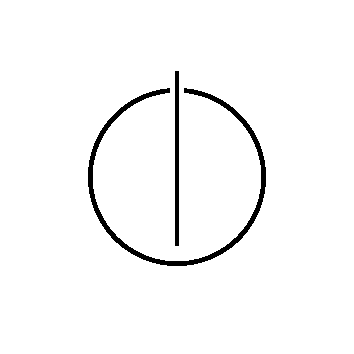
\includegraphics[width=4cm]{styles/informat.png}
  \end{figure}
  
  \end{center}
%	\clearemptydoublepage
%	
%	% The titlepage for the CAMP report document.
% Included by MAIN.TEX


%--------------------------------------------------
% The title page
%--------------------------------------------------

% correct BCOR - undo at the end !!!
\def\bcorcor{0.15cm}
\addtolength{\hoffset}{\bcorcor}

\thispagestyle{empty}

 \vspace{10mm}
\begin{center}
	       \oTUM{4cm}
	   
	   \vspace{5mm}     
	   \huge FAKULT{\"A}T F{\"U}R INFORMATIK\\ 
	   \vspace{0.5cm}
	 \large DER TECHNISCHEN UNIVERSIT{\"A}T M{\"U}NCHEN\\
        
	\end{center}
		

\vspace{10mm}
\begin{center}

   {\Large \doctype}

  \vspace{10mm}
  
  {\LARGE \title}\\
  
  
  \vspace{10mm}
  
  
  {\LARGE  \titleGer}\\
  
  
  \vspace{10mm}

    %\hfill
    \begin{tabular}{ll}
	   \Large Autor:     & \Large \author \\[2mm]
	   \Large Themensteller:    & \Large Prof. Alfons Kemper, Ph.D.\\[2mm]				
	   \Large Betreuer:	& \Large Tobias M\"uhlbauer, M.Sc.\\[2mm]
	   \Large Datum:       & \Large 16. Februar 2015
	 \end{tabular}
	 
	 \vspace{5mm}
	 
	 \begin{figure}[h!]
  \centering
   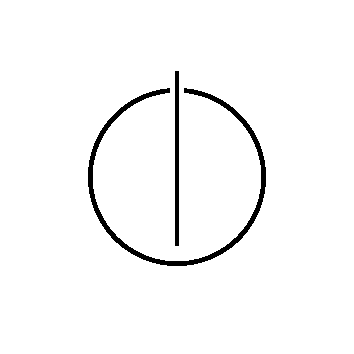
\includegraphics[width=4cm]{styles/informat.png}
  \end{figure}
   

\end{center}

% undo BCOR correction
\addtolength{\hoffset}{\bcorcor}

	
	
%	\input{components/cover_maschmeyer}
	\clearemptydoublepage
	
	% The titlepage for the CAMP report document.
% Included by MAIN.TEX


%--------------------------------------------------
% The title page
%--------------------------------------------------

% correct BCOR - undo at the end !!!
\def\bcorcor{0.15cm}
\addtolength{\hoffset}{\bcorcor}

\thispagestyle{empty}

 \vspace{10mm}
\begin{center}
	       \oTUM{4cm}
	   
	   \vspace{5mm}     
	   \huge FAKULT{\"A}T F{\"U}R INFORMATIK\\ 
	   \vspace{0.5cm}
	 \large DER TECHNISCHEN UNIVERSIT{\"A}T M{\"U}NCHEN\\
        
	\end{center}
		

\vspace{10mm}
\begin{center}

   {\Large \doctype}

  \vspace{10mm}
  
  {\LARGE \title}\\
  
  
  \vspace{10mm}
  
  
  {\LARGE  \titleGer}\\
  
  
  \vspace{10mm}

    %\hfill
    \begin{tabular}{ll}
	   \Large Autor:     & \Large \author \\[2mm]
	   \Large Themensteller:    & \Large Prof. Alfons Kemper, Ph.D.\\[2mm]				
	   \Large Betreuer:	& \Large Tobias M\"uhlbauer, M.Sc.\\[2mm]
	   \Large Datum:       & \Large 16. Februar 2015
	 \end{tabular}
	 
	 \vspace{5mm}
	 
	 \begin{figure}[h!]
  \centering
   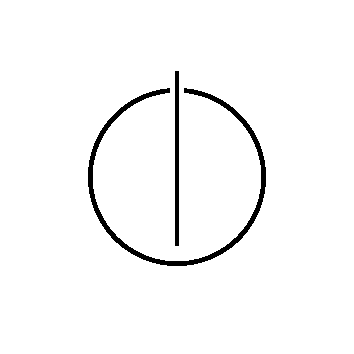
\includegraphics[width=4cm]{styles/informat.png}
  \end{figure}
   

\end{center}

% undo BCOR correction
\addtolength{\hoffset}{\bcorcor}

	
	
	\clearemptydoublepage


\thispagestyle{empty}
\selectlanguage{german}
	\vspace*{0.8\textheight}
	\noindent
	Ich versichere, dass ich diese Abschlussarbeit selbst{\"a}ndig verfasst und nur die angegebenen Quellen und Hilfsmittel verwendet habe.
	
	\vspace{15mm}
	\noindent
	M{\"u}nchen, den \today \hspace{5cm} \author
%\selectlanguage{english}
\newpage

	
%	\clearemptydoublepage
\phantomsection
\addcontentsline{toc}{chapter}{Acknowledgements}	


%\chapter*{Acknowledgements}

\vspace*{2cm}

\begin{center}
{\Large \bf Acknowledgments}
\end{center}

\vspace{1cm}




If someone contributed to the thesis... might be good to thank them here.

	
	% Abstract for the TUM report document
% Included by MAIN.TEX


\clearemptydoublepage
\phantomsection
\addcontentsline{toc}{chapter}{Abstract}	





\vspace*{2cm}
\begin{center}
{\Large \bf Abstract}
\end{center}
\vspace{1cm}

This work is about bash scripts analyzing flat files (commonly known as CSV files) that will be compared to SQL queries doing the same on relational databases.\\

Methods for analyzing data will be tested on their efficiency and how they could be a\-dap\-ted for use with relational databases.
That is why some useful familiar unix command line tools as well as newer innovations using the command line will be presented.
But in the end, it shows the disadvantage of common scripts in fields of duration and maintainability.\\

The first goal is a implementation of the TPC-H benchmark only using unix command line tools, afterwards a bash to SQL converter will be presented, which makes query processing on flat file databases much easier.\\

As a result of performance tests using TPC-H benchmarks, times about up to 15 minutes for processing a query, command line tools should be replaced by an equivalent SQL query.\\

The presented Bash2SQL compiler converts each command to SQL statements and con\-nects SQL queries, where their origin commands are in one pipeline. The produced SQL query can stand alone or be embedded in a new bash script.

%Performance tests on query processing on flat file databases using bash and on modern relational databases using SQL and developing a Bash to SQL compiler to substitute command line tools


	% Included by MAIN.TEX


\clearemptydoublepage






\vspace*{2cm}
\begin{center}
{\Large \bf Zusammenfassung}
\end{center}
\vspace{1cm}

Diese Arbeit beschäftigt sich mit Bash-Skripten, die tabellenähnliche CSV-Dateien auslesen, im Vergleich zu ihnen äquivalenten SQL-Abfragen, die auf relationalen Datenbanken arbeiten.\\

Wissenschaftliche Daten werden oft in textbasierten Formaten, etwa CSV, gespeichert, die meist mit Unix Werkzeugen analysiert werden. Oft sind diese in unverständliche Bash-Skripte verpackt, deren Ausführung viel Zeit in Anspruch nimmt.\\

Der Flaschenhals von Datenbanken ist das Laden der Daten, neue Technologien erlauben das Laden quasi in Echtzeit. Zudem erleichtern Datenbanken die Datenaufbereitung mittels einer leicht verständlichen Abfragesprache, die bei der Datenanalyse auch genutzt werden sollte. Daher untersucht diese Arbeit wie die Datenverarbeitung in der Wissenschaft durch den geeigneten Einsatz von relationalen Datenbanksystemen verbessert werden kann.\\

Hierbei problematisch ist die Portierung der Bash Skripte auf ein Datenbanksystem, denn müssen diese Analysen neu geschrieben werden, so ist ein Umstieg wenig reizvoll. Ein Compiler, der die Skripte automatisiert in SQL übersetzt, soll das ändern, weshalb diese Arbeit verfolgt, wie Skripte in äquivalente SQL-Abfragen übersetzt werden.\\

Zuerst wird der Geschwindigkeitsnachteil von Bash-Skripten anhand des TPC-H Benchmarks für analytische Anfragen verdeutlicht. Dazu werden die Anfragen mit Unix-Werk\-zeu\-gen implementiert und Laufzeiten von bis zu 15 Minuten pro Abfrage auf 10\ GB großen Daten gemessen.\\

Um bestehende Analysen aus Bash-Skripten im Einsatz mit relationalen Da\-ten\-bank\-sys\-te\-men weiterhin nutzen zu können, wird die Idee eines Konverters zu SQL betrachtet, der Skripte automatisiert in SQL transferiert.
Der entwickelte Bash2SQL-Compiler übersetzt jedes Kommando in eine SQL-Abfrage und verschachtelt über eine Pipeline verbundene Kommandos, sodass am Ende ein gültiger SQL-Ausdruck entsteht, eventuell eingebunden mittels eines SQL-Kommandos in ein Bash-Skript.



	\tableofcontents
  
%	\clearemptydoublepage

\phantomsection
\addcontentsline{toc}{chapter}{Outline of the Thesis}

\begin{center}
	\huge{Outline of the Thesis}
\end{center}




%--------------------------------------------------------------------
\section*{Part I: Introduction and Theory}

\noindent {\scshape Chapter 1: Introduction}  \vspace{1mm}

\noindent  This chapter presents an overview of the thesis and it purpose. Furthermore, it will discuss the sense of life in a very general approach.  \\

\noindent {\scshape Chapter 2: Theory}  \vspace{1mm}

\noindent  No thesis without theory.   \\

%--------------------------------------------------------------------
\section*{Part II: The Real Work}

\noindent {\scshape Chapter 3: Overview}  \vspace{1mm}

\noindent  This chapter presents the requirements for the process.


	\mainmatter
	
	
		% ---------------------------------------------------------------------------
		%
		%Introduction and Background Theory
		%
		% ---------------------------------------------------------------------------
		%\part[Motivation]{Motivation}
		\label{part:introAndBackgroundTheory}
		\chapter{Einführung}
\label{chapter:Einfuhrung}
\section{Motivation}
Die Welt wächst zusammen, die Kommunikation steigt und mit ihr auch das Datenvolumen. Waren es 2005 geschätzte 130 Exabyte (130 Mrd. GB) an erzeugten Daten weltweit, so hat sich die Menge bis 2012 um das 20-fache auf 2837 Exabyte gesteigert und 2015 soll die Marke der Zettabyte gebrochen werden, ganze 40000 Exabyte werden an Daten erwartet, die Menge verdoppelt sich jährlich \cite{statista}.\\
%Der Begriff Big Data ist weit gefasst, verstehen die meisten darunter den Rohstoff zur Analyse digitaler Profile von Menschen, so sind ihr Kern doch Daten, denn das Potential der Digitalisierung steigt ins Unermessliche.
%Daten werden maschinell generiert, allein mit RFID-Chips werden Tiere gebrandmarkt, Menschen geben ihre Arbeitszeiten durch, selbst Mülltonen werden damit gekennzeichnet. Neue Technologie ergibt bessere Sensoren mit automatisierteren Abläufen, damit nützt sie vor allem der Forschung: noch mehr Ergebnisse, noch genauere Vorhersagen machen noch präziseres Reagieren in Klimaforschung, Geologie und Physik möglich.\\
Für den Austausch benötigt man die Daten und damit ein geeignetes Datenformat, eines hat sich schlichtweg durchgesetzt: die CSV-Datei - ein portables und menschenlesbares Format zur Darstellung tabellen-ähnlicher Daten.
Aber zur Analyse allein reicht ein Datenformat nicht aus, es müssen Abfragen darüber laufen, die einem Zugriff verschaffen. Die Lösung sind ganz klar relationale Datenbanken mit einer eigenen Abfragesprache, dennoch scheint unter Wissenschaftlern und Firmen eine Ablehnung gegenüber proprietären Datenbanksystemen zu herrschen, da sie ihre Daten lieber in Textform und CSV-Dateien halten.\\
Schaut man in einem Standardwerk zur Datenhaltung für Geowissenschaftler nach, so schlägt es gleichrangig zwei Konzepte vor: textbasierte Datenbanken (wie CSV-Dateien) und relationale Datenbanken. Der anschließende Vergleich erkennt: textbasierte Datenbanken benötigen zum Zugriff "`ein Skript, dass die Datei öffnet und in der ganzen Datei sucht"' \cite[S. 19]{Geo}.
Diese Skripte sind auf unixoiden Systemen meist Bash-Skripte die schwierig zu schreiben, zu warten und in der Ausführung sehr langsam sind.\\
Doch zurück zu großen Datenmengen, was passiert wenn die Daten zu groß werden? Die Abfragezeit mit Skripten explodiert. Will man ein Datenbanksystem zu Hilfe ziehen, so unterstützen sie CSV-Dateien nur unzureichend, sie müssen zuerst geladen werden oder, wie es Oracle anbietet, als \textit{external table} in die Datenbank eingebunden, beides ist teuer.
Programme, die für den CSV-Import in Datenbanken sorgen, gibt es genügend.
Darum stellt diese Arbeit ein Verfahren vor, wie Skripte in SQL-Abfragen umgewandelt werden.
\begin{figure}
\centering
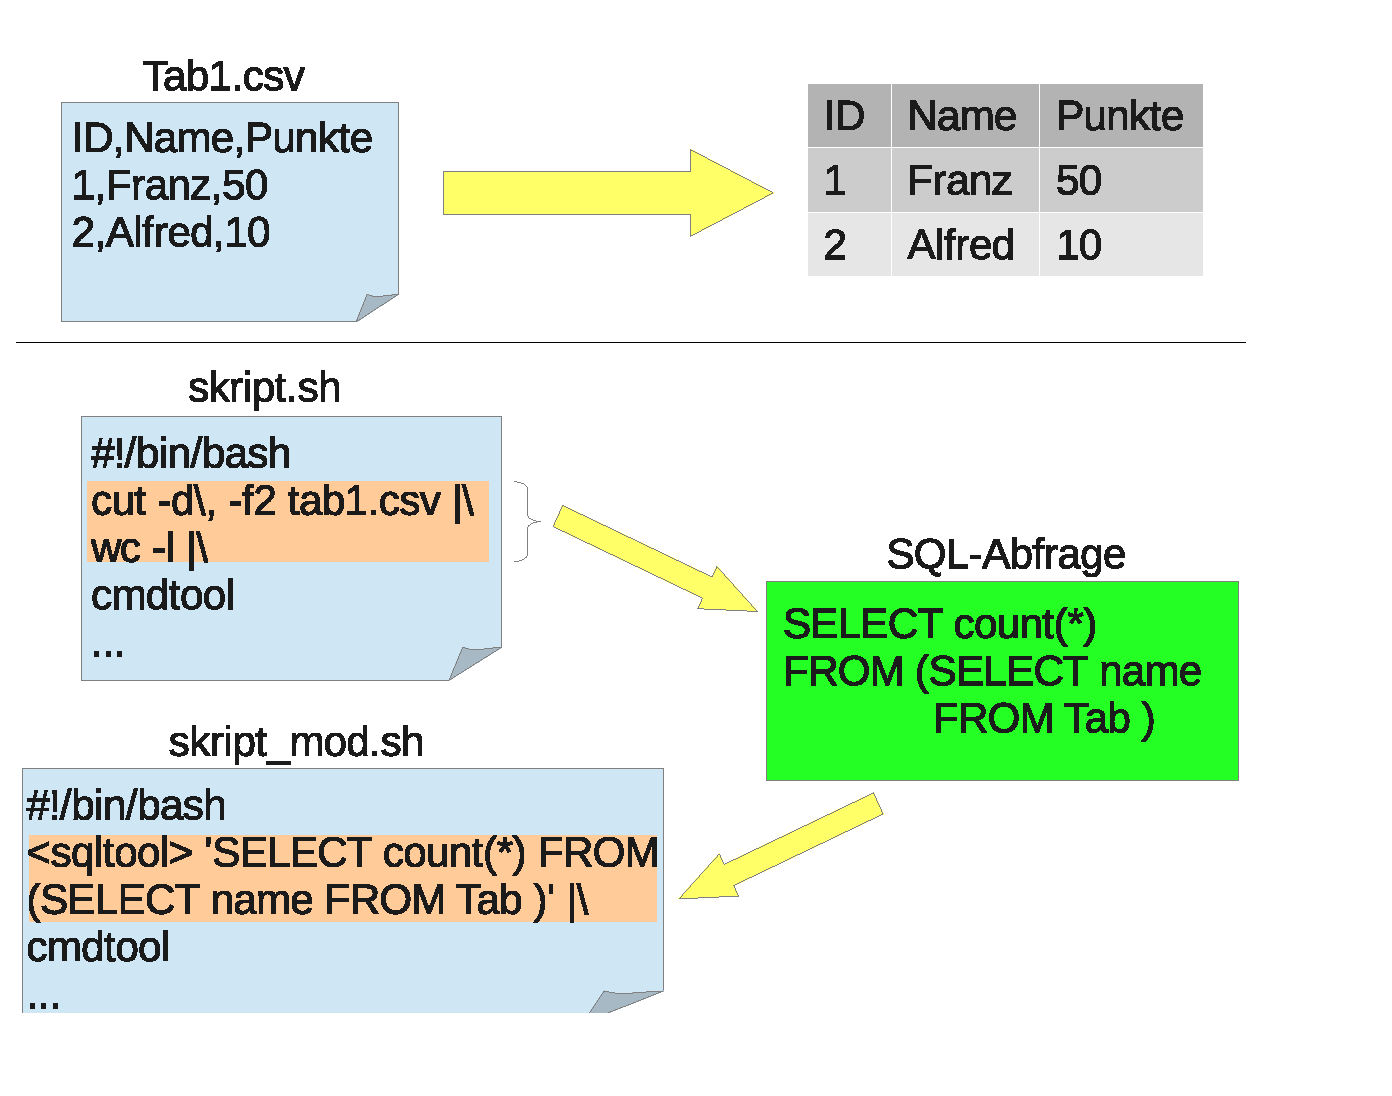
\includegraphics[scale=.5]{idee}
\caption{Grundidee: Daten werden vorab in eine Datenbank geladen, anschließend werden die Skripte übersetzt}
\label{fig:idee}
\end{figure}
Jetzt wird das Beste aus beiden Welten kombiniert - Bash-Skripte mit SQL-Abfragen. Soweit wie möglich sollen alle Kommandos eines Skripts in eine äquivalente SQL-Anweisung übersetzt werden. Um dennoch die Funktionen eines Skripts nicht zu verlieren, soll es möglich sein, die Abfrage in das Skript mittels eines Kommandos einzubinden, das die Abfrage auf einer Datenbank ausführt (\textit{SQL inline}).
Dazu wird ein Übersetzer geschrieben, der Shell-Skripte einliest und sie komplett oder teilweise in SQL-Abfragen übersetzt (siehe Abb. \ref{fig:idee}). So können die Vorteile eines Datenbanksystems mit einer einfachen deklarativen Sprache (SQL), mit parallelisierter Anfrageverarbeitung und deren Geschwindigkeit ausgenutzt werden, die Speicherung der Daten erfolgt aber weiterhin in CSV-Dateien.\\

\section{Textbasierte Datenbanken}
%Das Jahr 1970 bedeutete einen Umbruch im Bereich der Datenbanken, Edgar F. Codd veröffentlichte sein Papier über das relationale Modell, der Grundlage aller relationaler Datenbanken. Es erlaubt, mehrere Relationen zu verbinden, ohne dass der Benutzer sich um die interne Repräsentation kümmern muss \cite{Codd70}.
%Dennoch dauerte es weitere neun Jahre bis Larry Ellison und Bob Miner den ersten Prototyp einer relationalen Datenbank mit ihrer Firma Software Development Laboratories auf den Markt brachten, bei IBM sogar zwei Jahre länger \cite{Henderson03}.
%Dennoch werden Datensätze gerne noch in textbasierten Datenbanken (engl.: flat file databases) wie CSV-Dateien wegen ihrer Einfachheit gespeichert.\\

\begin{figure}[htb]
\centering
\begin{tabular}{p{3,5cm}|p{7,5cm}}
\hline
Franz Winkler & Am Winkl 5, 80000 Musterstadt\\ \hline
Xaver Ziegler & Maurergasse 19, 80000 Musterstadt\\ \hline
\end{tabular}
\caption{Beispiel für textbasierte Datenbank}
\end{figure}

%Textbasierte Datenbanken gibt es schon immer, sobald eine Person ein Adressbuch von Kontakten mit Namen und Adressen pflegt, so ist das eine textbasierte Datenbank. Sobald ein Kontakt den Wohnsitz wechselt oder die Anzahl an Freunden wächst, muss die Datenbank aktualisert werden, ist sie geordnet, bedeutet das in manchen Fällen, die Daten komplett neuzuschreiben, ein unnötiger Aufwand.\\
%Mit diesem Problem konfrontiert hat der deutschstämmige US-Amerikaner Hermann Hollerith bereits 1884 das erste Datenformat erfunden, \cite[S.48]{Bioinf08}, abgeschaut von Schaffnern in Zügen, die die Fahrkarten an bestimmten Stellen gelocht haben um Wiederverwendung auszuschließen, hat er die Lochkarte entwickelt. Das System wurde 1890 erstmals bei einer Volkszählung eingesetzt, wobei die Lochkarten die Informationen über Geschlecht und Alter enthielten und elektrische Maschinen in 3,4 Sekunden eine Karte auslasen. Weitere Aufträge auf der ganzen Erde folgten, Hollerith gründete die Computing Tabulating Recording Company (CTR), aus der 1924 schließlich IBM hervorging \cite{Heise07}.\\

%\begin{figure}
%\centering
%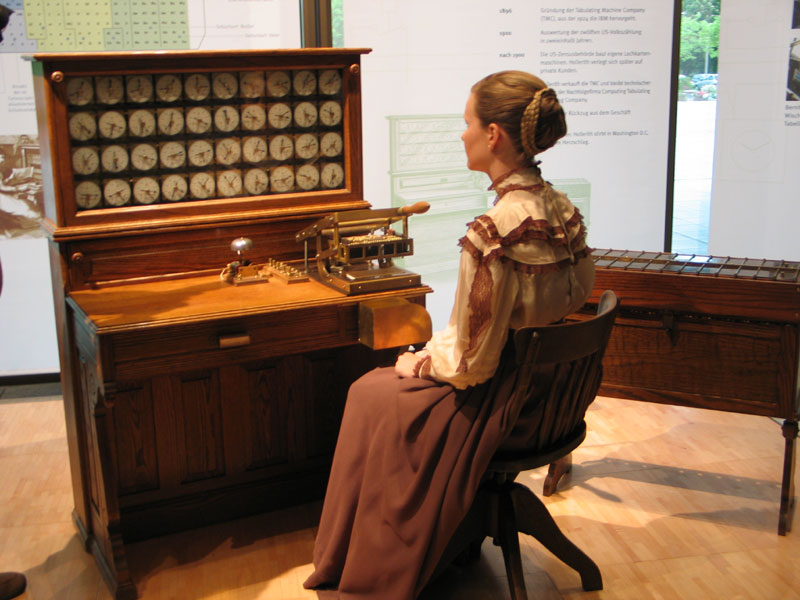
\includegraphics[scale=.2]{hollerith_machine.jpg}
%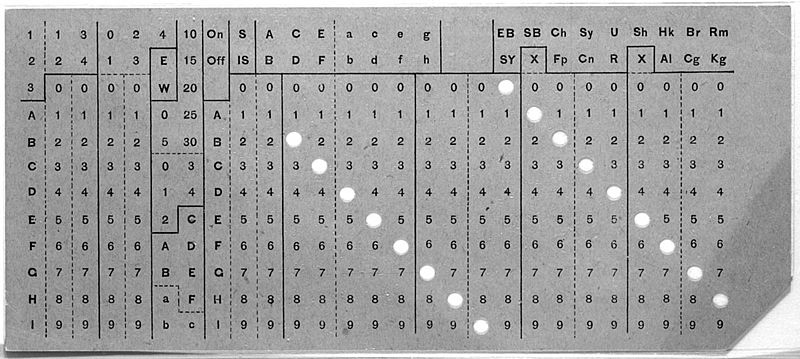
\includegraphics[scale=.7]{Hollerith_Punched_Card.jpg}
%\caption{Hollerith Maschine \cite{Heise07} mit Lochkarte [wikipedia.de]}
%\label{fig:hollerith}
%\end{figure}

%Textbasierte Datenbanken sind mittlerweile weit verbreitet, in Unix-Systemen (entwickelt Mitte der 1960-er Jahre) werden so Daten zum Beispiel zur Passwort- oder Gruppenverwaltung gespeichert. (siehe Abb. \ref{fig:passwd})
%Jeder Datensatz wird durch einen Zeilenvorschub mit Wagenrücklauf (engl.: carriage return und line feed, CRLF) abgeschlossen, einzelne Felder durch ein Trennzeichen (engl.: delimiter) separiert \cite{cql}. \\

%\begin{figure}
%\centering
%\fbox{\parbox{15cm}{
%root:x:0:0:root:/root:/bin/bash\\
%daemon:x:1:1:daemon:/usr/sbin:/bin/sh\\
%bin:x:2:2:bin:/bin:/bin/sh\\
%sys:x:3:3:sys:/dev:/bin/sh\\
%sync:x:4:65534:sync:/bin:/bin/sync
%}}
%\caption{Auszug aus /etc/passwd eines Unix-Systems mit Trennzeichen ':'}
%\label{fig:passwd}
%\end{figure}

Ein Beispiel für textbasierte Datenbanken sind CSV-Dateien (Comma-Separated Values) manchmal auch DSV-Dateien (Delimiter-Separated Values) genannt, also durch Komma oder anderes Trennzeichen separierte Tabellen. Erstmals zwischen 1968 und 1972 erwähnt als Teil der Fortran Spezifikation für listenorientierte Ein- und Ausgabe (Common Format and MIME Type for Comma-Separated Values (CSV) Files) \cite[S. 17]{IBM_Fortran}, haben sich CSV-Dateien zum Standard im Datenaustausch entwickelt.\\

Inzwischen existiert sogar eine Richtlinie für CSV-Dateien, herausgegeben von der Internet Engineering Task Force in der RFC\ 4180. Nach dieser Richtlinie soll jeder Datensatz einer CSV-Datei durch einen Zeilenvorschub mit Wagenrücklauf (engl., carriage return und line feed, CRLF) abgeschlossen und einzelne Felder durch ein Trennzeichen (engl.,\ delimiter) separiert sein \cite{RFC}.\\

Da die Richtlinie sich an DOS-Systemen (mit CRLF, '\textbackslash r\textbackslash n') orientiert, verwenden andere Systeme einen einfachen Zeilenvorschub (LF, '\textbackslash n'). Für gewöhnlich bestehen CSV-Dateien aus einem systemabhängigem Record Delimiter (zum Trennen von Datensätzen) und einem variablen Field Delimiter (Spaltentrennzeichen wie Komma) und orientieren sich an folgendem Schema:
\begin{itemize}
\item jeder Datensatz ist in einer Zeile gespeichert, beendet durch einen Record Delimiter
\item der letzte Datensatz benötigt keinen Record Delimiter
\item die erste Zeile kann eine Kopfzeile (engl., header) sein und muss für jede Spalte einen String als Bezeichner enthalten
\item die Felder sind durch einen Field Delimiter getrennt, nach der letzten Spalte muss kein Field Delimiter folgen; Leerzeichen sind Teil eines Feldes
\item jedes Feld kann in Anführungszeichen (doppelte Hochkommata, engl., double quoted fields) stehen
\item ein Feld, das Field Delimiter oder Record Delimiter enthält, muss in Anführungszeichen eingeschlossen sein
\item Anführungszeichen als Inhalt eines Feldes in doppelten Hochkommata (double quoted fields) werden escaped (durch eine Fluchtsequenz, z.B. '\textbackslash ')
\end{itemize}

Die Vorteile solcher Datenbanken liegen in ihrer Einfachheit, sie speichern alle Informationen, es werden keine weiteren Informationen benötigt, Import und Export von Informationen ist leicht, da außer einem Field bzw. Record Delimiter keine Konventionen einzuhalten sind.\\

Die Nutzung textbasierter Datenbanken bei Abfragen birgt aber Nachteile, so lassen sich die Daten speichern und verschicken, ein Ändern einzelner Datensätze erweist sich als schwierig, ohne die komplette Datei zu überschreiben. Da das Format nur wenigen Beschränkungen unterliegt, enthält in manchen Fällen die erste Zeile die Feldbezeichner, in anderen bereits den ersten Inhalt.
Aber das gravierendere Problem liegt in der Anzahl der Datensätze, jeder Datensatz muss zeilenweise ausgelesen werden, da auch keine Konventionen befolgt werden, ist auch nicht von einer Sortierung auzugehen. Analysen oder Datenänderungen sind auf diesem Format schwieriger und kostenaufwändiger als auf anderen, z.B. binär gespeicherten Daten.

\section{Vorgehen}
Im Nachfolgenden werden zuerst grundlegende Befehle erklärt, wie sie in Skripten zur Analyse von Textdateien vorkommen und auf bereits existierende Ansätze verwiesen, wie Daten in Textdateien bewältigt werden. Abschließend führt die Arbeit in die Welt der Parser und zeigt einen Ansatz auf, wie die Skripte übersetzt werden.

		
		
		%
		%% ---------------------------------------------------------------------------
		%%
		%% Fully Automated Calibration for Ultrasound
		%%
		%%% ---------------------------------------------------------------------------
		%\part[Bash]{Bash statt SQL}
		%\label{part:secondP}
		
\chapter{Bash statt SQL}
Um die Bash-Kommandos zu ersetzen, wird zuerst die Idee benötigt, wie sieht eine SQL-Anfrage in der Bash ausgedrückt mithilfe der klassischen Unix-Befehle aus, die textbasierte Datenbanken auslesen. Daher erklärt dieses Kapitel zuerst, wie Analysen auf Textdateien mit Kommandos wie cat, cut, awk und sed analog zu SQL-Abfragen aussehen. Anschließend werden damit Datenbank-Benchmarks implementiert und die Zeit der Abfragen bei großen Datenmengen gemessen. Der Vergleich mit neueren Programmen erfolgt dann im nächsten Kapitel.

\begin{figure}[htb]
\centering
Punktetabelle: \hspace{6cm} Zeittabelle:\\
\begin{tabular}{p{1cm}|p{3cm}|p{1cm}}
\hline
ID & Name & Punkte \\ \hline
1 & Franz & 50 \\ \hline
2 & Alfred & 10 \\\hline
3 & Marie & 27 \\\hline
\end{tabular}
\hspace{3cm}
\begin{tabular}{p{1cm}|p{1cm}}
\hline
ID & Zeit\\ \hline
1 & 44 \\ \hline
2 & 88 \\\hline
3 & 67 \\\hline
\end{tabular}
\caption{Beispiel Datenbank}
\label{fig:bspDB}
\end{figure}

\section{Relationale Algebra der Unix-Shell im Vergleich zu SQL}
Welche Strukturen eines Shell-Skripts sind in welche SQL-Anweisungen zu übersetzen? Um dies besser vergleichen zu können, werden im Folgenden Ausdrücke der relationalen Algebra als Befehle der Unix-Shell ausgedrückt und eine äquivalente Abfrage in SQL angegeben. Als Grundlage für die relationale Algebra dienen Operatoren aus dem Buch Datenbanksysteme \cite{Kemper} und in diesem Kapitel werden ausschließlich die grundlegenden Kommandos der Unix-Shell verwendet, heute auch bekannt als GNU core utilities \cite{Gulbins}.
\subsection{Grundlage}
Die Ausgabe einer Tabelle in SQL ist recht schlicht.
\begin{lstlisting}[language=SQL]
 SELECT * FROM Punktetabelle
\end{lstlisting}
Für die Ausgabe einer Textdatei in der Shell dienen Befehlen wie \textit{cat}, \textit{more}, \textit{less}, ... Sie finden sich häufig, wenn vorher Daten durchgepiped werden.
\begin{lstlisting}[language=Bash]
 cat Punktetabelle;
\end{lstlisting}
\subsection{Selektion}
Wenn jetzt Tupel ausgewählt werden, die ein Prädikat erfüllen sollen, dann ist dies eine Selektion und es sind zwei Fälle zu unterscheiden:
Äquivalenz: $\sigma_{ID=3}(Tabelle)$ oder Vergleich $\sigma_{ID<3}(Tabelle)$ oder in SQL:\\
\begin{lstlisting}[language=SQL]
 SELECT * FROM Punktetabelle WHERE ID=3;
 SELECT * FROM Punktetabelle WHERE ID<3
 SELECT * FROM Punktetabelle WHERE Name='Marie'
\end{lstlisting}

Die allgemeine Lösung nutzt \textit{awk}, mit dem alle Vergleichsfunktionen einer höheren Programmiersprache implementiert sind, hierbei sind die Felder durch \textit{\$1,...,\$n} bezeichnet, \textit{\$0} steht für alle Felder, die Option \textit{-F,} bezeichnet das Feldtrennzeichen (Delimiter), anschließend folgt ein Muster und der Befehl, der ausgeführt wird (\textit{' pattern \{CMD\}'}), in diesem Fall zuerst die Bedingung \textit{\$1==3} und der Befehl zur Ausgabe, \textit{print \$0} gibt alle Spalten aus (das \textit{SELECT *} der SQL).
\begin{lstlisting}[language=Bash]
$ awk -F, '$1==3 { print $0 }' Punktetabelle.csv
$ awk -F, '$1>3  { print $0 }' Punktetabelle.csv
$ awk -F, '$2="Marie" { print $0 }' Punktetabelle.csv
\end{lstlisting}

Andere grundlegende Kommandos funktionieren meist nur bei kompletter Äquivalenz, wie \textit{grep}, das in einer Datei nach allen Vorkommen der gewünschten Zeichenfolge sucht. Bei \textit{sed} kann auch auf Äquivalenz geprüft werden, dabei ist es aber von Vorteil, zumindest den vorderen und hinteren Spaltentrenner mit anzugeben, oder gar alle möglichen:
\begin{lstlisting}[language=Bash]
$ grep -r '3,.*' Punktetabelle.csv
$ grep -r 'Marie' Punktetabelle.csv
$ sed -nr '/3,.*/p' Punktetabelle.csv
$ sed -nr '/Marie/p' Punktetabelle.csv
\end{lstlisting}

\subsection{Projektion}
Wenn nun einzelne Spalten ausgewählt werden, so wird die Projektion benötigt:\\
{$\Pi_{Name,Punkte}(Punktetabelle)$}\\

oder in SQL:
\begin{lstlisting}[language=SQL]
 SELECT Name FROM Punktetabelle
\end{lstlisting}
Das klassische Unix-Kommando dazu ist \textit{cut}, das es mit Hilfe der Option \textit{-f} erlaubt, einzelne Felder zu extrahieren, Felder werden beginnend beim ersten durch Aufzählung mit Kommata bestimmt (1,3) und ganze Bereiche mit Bindestrich ausgewählt (1-3 entspricht Feldern eins bis drei), der Spaltentrenner wird durch die Option \textit{-d} mitgeteilt (Standard: Leerzeichen).
\begin{lstlisting}[language=Bash]
$ cut -f2,3 -d, Punktetabelle.csv
\end{lstlisting}
Die Kommandos \textit{awk} und \textit{sed} erlauben die Projektion auch, ersterer Befehl einfach mit \textit{print}, bei sed müssen explizit die Spaltentrenner angegeben werden:
\begin{lstlisting}[language=Bash]
$ awk -F, '{print $2,$3}' OFS=, Punktetabelle.csv
$ sed -nr 's/([^,]*),([^,]*),(.*)/\2\3/p'
\end{lstlisting}
\subsection{Vereinigung}
Die Vereinigung $\Pi_{ID}(Punktetabelle) \cup \Pi_{ID}(Zeittabelle)$ ist am einfachsten in der Unix-Shell zu realisieren, schließlich unterstützt fast jeder Befehl durch Eingabe mehrerer Dateien das Zusammenfügen dieser. Für das Zusammenfügen oder Konkatenieren drängt sich \textit{cat} (concatenate) geradezu auf, dadurch definiert sich doch dieser, einfach alle Dateien der Reihe nach auflisten:
\begin{lstlisting}[language=Bash]
$ cat datei1 datei2
\end{lstlisting}
Und schon sind sie vereinigt, analog das Beispiel der oben gezeigten Projektion:
\begin{lstlisting}[language=SQL]
 SELECT ID FROM Punktetabelle
 UNION
 SELECT ID FROM Zeittabelle
\end{lstlisting}
Das Beispiel erfordert vorher die Selektion, daher werden zwei anonyme Pipes verwendet, das sieht dann so aus:
\begin{lstlisting}
$ cat <(cut -f1 -d, Punktetabelle.csv) \
	<(cut -f1 -d, Zeittabelle.csv)
\end{lstlisting}

\subsection{Kreuzprodukt}
Will man in der Shell das Kreuzprodukt
$Punktetabelle \times Punktetabelle$
bilden, so geschieht das in SQL durch Auswahl mehrerer Tabellen:
\begin{lstlisting}[language=SQL]
 SELECT * FROM Punktetabelle, Punktetabelle
\end{lstlisting}
In der Shell hilft einem auch hier \textit{awk} weiter, diesmal mit Feldern. Zuerst werden alle Eingabezeilen (leeres Suchmuster) oder nur die gewünschten wie bisher durchgegangen und in dem Feld aufsteigend gespeichert. 
Anschließend, also im Schlussteil (bezeichnet durch END), kann mit den Feldern alles produziert werden, das Kreuzprodukt erfolgt durch die Ausgabe mit print in einer doppelten For-Schleife.
\begin{lstlisting}[language=Bash]
cat Punktetabelle | awk -F\| '
        {
		lines[i++]=$0
        }
        END{
                for (i in lines)
                  for (j in lines)
                    print lines[i], lines[j]
        }
' OFS=,
\end{lstlisting}
\subsection{Mengendifferenz}
Um alle Mengenoperationen der Algebra abzudecken, wird auch noch die Differenz benötigt, geschrieben als $R-S$, zum Beispiel ergibt $\Pi_{ID}(Punktetabelle) - \Pi_{ID}(Zeittabelle)$ diejenigen Tupel, zu denen kein passender Eintrag in der Zeittabelle einthalten ist.
\begin{lstlisting}[language=SQL]
 SELECT ID FROM Punktetabelle
 EXCEPT
 SELECT ID FROM Zeittabelle
\end{lstlisting}
In der Unix-Shell gibt der Befehl \textit{comm} die Zeilen in drei Spalten aus, zuerst die nur der ersten Datei (1), dann die nur der Zweiten (2) und dann die aus beiden (3), durch Angabe der Zahlen, können die Spalten unterdrückt werden. Für den Vergleich müssen die Dateien aber sortiert sein.
Analog zur Algebra entspricht folgender Befehl der Differenz:
\begin{lstlisting}[language=Bash]
$ comm -23 R S
\end{lstlisting}
Angewandt auf die Beispieltabellen:
\begin{lstlisting}[language=Bash]
$ comm -23 <(cut -f1 -d, Punktetabelle.csv | sort) \
		 <(cut -f1 -d, Zeittabelle.csv | sort)
\end{lstlisting}

\subsection{Umbennenung}
Um alle Ausdrücke der relationalen Algebra abzudecken, fehlt nun noch die Umbenennung der Tabelle $\rho_{t1}(Punktetabelle)$ und einzelner Spalten $\rho_{Nr \leftarrow ID}(Punktetabelle)$. Da in der Shell die Tabellen nichts anders als Datenströme sind, ist keine Unterscheidung der Namen notwendig, eine Möglichkeit, die Tabellen umzubenennen, besteht nur darin, eine temporäre Hilfstabelle mit neuem Namen anzulegen.
\begin{lstlisting}[language=Bash]
$ cp Punktetabelle.csv t1.csv
\end{lstlisting}
Auch einzelne Spalten können nur mit ihrer Nummer angesprochen werden (\$1,\$2, etc.), eine Umbenennung kann nur für die Ausgabe erfolgen, der Strom muss also vorher mit \textit{awk} oder \textit{sed} bearbeitet werden.
\begin{lstlisting}[language=Bash]
$ sed -r 's/ID/Nr/' Punktetabelle.csv 
NR,Name,Punkte
1,Franz,50
2,Alfred,10
3,Marie,2
$ cat Punktetabelle | awk -F\| '
        NR==1{
		print "Nr", $2, $3
        }
        NR>2{
		print $0
	}
' OFS=,
\end{lstlisting}

\subsection{Relationaler Verbund}
Alle grundlegenden Operatoren der relationalen Algebra können auch mit einfachen Skripten auf textbasierten Datenbanken erfolgen, dennoch darf ein wichtiger Operator nicht fehlen, der relationale Verbund (Join), vor allem der natürliche Verbund (natural join), der Tabellen über Äquivalenz zusammengehöriger Attribute verknüpft:\\

$R \Join S $ 

oder im Beispielfall mit Verknüpfung über ID: $ Punktetabelle \Join Zeittabelle$\\
Der analoge Fall in SQL:
\begin{lstlisting}[language=SQL]
 SELECT *
 FROM Punktetabelle, Zeittabelle
 WHERE Punktetabelle.ID = Zeittabelle.ID
\end{lstlisting}

In Unix stehen für Equijoins jeglicher Art, bei denen jeweils ein Feld jeder Tabelle übereinstimmen soll, das Kommando \textit{join} zur Verfügung. Sollen zwei CSV-Dateien miteinander verknüpft werden, so müssen das Spaltentrennzeichen und die zu verknüpfenden Spalten (\textit{-1 spalteA -2 spalteB}) angegeben werden, standardmäßig der Leerraum (Whitespace) sowie die jeweils erste Spalte, und, sofern die erste Zeile die Bezeichner enthält, müssen diese als solche mit \textit{--header} deklariert sein.
\begin{lstlisting}[language=Bash]
$ join --header -t, -1 1 -2 1 Punktetabelle.csv Zeittabelle.csv
\end{lstlisting}
Zu beachten ist, dass im Ergebnis eine der verbundenen Spalten dann fehlt, also oben stehende Abfrage produziert folgendes Ergebnis:\\

\hspace{3cm}
\begin{tabular}{p{1cm}|p{3cm}|p{1.2cm}|p{1cm}}
\hline
ID & Name & Punkte & Zeit	 \\ \hline
1 & Franz & 50 & 44       \\ \hline
2 & Alfred & 10  & 88       \\\hline
3 & Marie & 27 & 67       \\\hline
\end{tabular}
\\\\
Die auszugebenden Spalten können auch hinter der Option \textit{-o} explizit angegeben werden, \textit{0} ist die verbundene Spalte, alle anderen mit der Spaltenummer der jeweiligen Tabelle, \textit{2.3} meint die dritte Spalte der zweiten Tabelle.
Also sollen die Spalten, für die die Join-Bedingung gilt, angezeigt werden und die zweite und dritte, so hilft folgender Befehl:
\begin{lstlisting}[language=Bash]
$ join -t, -o 0 1.2 1.3 tabelleA tabelleB
\end{lstlisting}
Damit können auch Semi-Joins $ R \ltimes S $ und $ R \rtimes S $ produziert werden, indem die Spalten angegeben sind, für einen linken Semi-Join sind das \textit{-o 1.1 1.2 \dots 1.n} und  für den rechten \textit{-o 2.1 2.2 \dots}\\

Ein Join der Shell ist ein Sort-Join, er funktioniert (wie \textit{comm} auch) nur auf sortierten Dateien, folglich muss oft eine Sortierung mit \textit{sort} erfolgen, bevor gejoint werden kann. Das Kommando \textit{sort} arbeitet mit Quicksort \cite{Prince}, also mit Durchschnittslaufzeit $O(n\ log\ n)$, in schlechten Fällen auch $O(n^2)$. Dabei muss der Sortierfunktion noch das Trennzeichen (\textit{-t,}) sowie die zu sortierenden Spalten als Feld angegeben werden, also \textit{-k2,3} sortiert nach dem zweiten und dritten Feld. Erfolgt ein Join danach, so ist zu empfehlen, nach exakt einer Spalte zu sortieren \textit{-k2,2}, da das Ergebnis sonst von der Länge des nachfolgenden Textes abhängt. 
\begin{lstlisting}[language=Bash]
$ sort -t, -k2,2 tabelleA | join -1 2 - tabelleB
\end{lstlisting}
\textit{sort} sortiert aber auch die Kopfzeile mit, also muss diese separat behandelt werden, am besten wird die erste Zeile mit \textit{head} extrahiert, alle anderen mit \textit{tail} und nach dem Sortieren können die Zeilen wieder zusammengefügt werden.
\begin{lstlisting}$
$ head -1 tabelleA > nurKopf
$ tail -n+2 tabelleA | sort -t, -k1,1 | cat nurKopf - > tabAmod
$ head -1 tabelleB > nurKopf2
$ tail -n+2 tabelleB | sort -t, -k1,1 | cat nurKopf2 - |\
  join -t, -1 1 -2 1 tabAmod - 
\end{lstlisting}

%Outer join äußerer Join (links und recht und alles), Antijoin
%
Auch der Antijoin $ R \vartriangleright S $ bzw. $ R \vartriangleright S$ ist in der Unix-Shell mit der Option \textit{-v1} und \textit{-v2} implementiert, der die Zeilen der ersten Tabelle (bzw. der zweiten) ausgibt, zu denen kein Partner in der anderen Tabelle gefunden wurde. Damit nur die benötigten Spalten ausgegeben werden, empfiehlt es sich, die Spalten mit der Option \textit{-o} noch explizit anzugeben:
\begin{lstlisting}[language=Bash]
$ join -t, -1 1 -2 1 -v1 -o 0 1.2 1.3 R.csv S.csv
\end{lstlisting}
Wenn zum Beispiel die Namen ausgegeben werden sollen, zu denen keine Zeit gemessen wurde, sieht das so aus:
\begin{lstlisting}
$ join -t, -1 1 -2 1 -v1 -o 1.2 Punktetabelle.csv Zeittabelle.csv
\end{lstlisting}

Als einzige Join-Arten, die noch fehlen, verbleiben die äußeren Joins
$R {\tiny \textifsym{d|><|d}} S $,
$R {\tiny \textifsym{d|><|}} S $ und
$R {\tiny \textifsym{|><|d}} S $,
die auch der Unix-Befehl mit der Option \textit{-a1} und \textit{-a2} erzeugt, wodurch alle Zeilen der ersten (analog der zweiten) Datei ausgegeben werden, auch solche mit fehlendem Join-Partner. Die fehlenden Werte, bei SQL die Null-Werte, können mit \textit{-e "Wert"} angegeben werden, sollen sie mit "'0"' aufgefüllt werden, dann mit \textit{-e "0"}.

\begin{lstlisting}[language=Bash]
$ join -t, -a1 -a2 -1 2 -2 2 -o 0 1.1 2.1 -e "0" tabelleR tabelleS
$ join -t, -a1     -1 2 -2 2 -o 0 1.1 -e "0" tabelleR tabelleS
$ join -t,     -a2 -1 2 -2 2 -o 0 2.1 -e "0" tabelleR tabelleS
\end{lstlisting}

\subsection{Gruppierung und Aggregation}
Über die relationale Algebra hinaus, geht der Gamma-Operator, der die Werte gruppiert und Aggregatsfunktionen wie max, min, sum oder avg auf ihnen erlaubt.
So gibt\\
$\gamma_{count(*)}(Punktetabelle)$
die Anzahl aller Teilnehmer aus. Aus dem Standard-Reportoire der Unix-Shell ist auch der Befehl \textit{awk} nützlich: Dazu sollten die Dateien vorher nach den Feldern sortiert sein, der Trick nutzt die Sortierung aus, die Werte der Spalten, nach denen gruppiert wird, wird vermerkt, die Aggregierung beginnt. Sobald sich ein Wert verändert, ist also zur nächsten Gruppe gesprungen worden, die aggregierten werden ausgegeben, die nächste Gruppe folgt, bis schließlich keine Zeilen mehr nachkommen, im END-Teil werden die letzten Aggregate ausgegeben.

\begin{lstlisting}[language=SQL]
SELECT spalte2, spalte3,
	max(spalte4), min(spalte4), count(*), avg(spalte4)
FROM Tabelle
GROUP BY spalte2, spalte3
\end{lstlisting}

Eine Gruppierung in \textit{awk} benutzt temporäre Variablen für die Summe, die Anzahl, das Minimun und das Maximum, der Durchschnitt setzt sich später aus Summe und Anzahl zusammen.
Zudem werden die Werte gespeichert, nach denen gruppiert wird. Ändern sich diese nicht, so werden die Werte der aktuellen Zeile in der Aggregation ergänzt, \textit{count} wird inkrementiert, der entsprechende Wert zur Summe von \textit{sum} addiert und nach größer und kleiner für \textit{min} und \textit{max} geschaut. Passen die Werte zum Gruppieren nicht überein, so werden die alten ausgegeben und die Aggregationsvariablen zurückgesetzt.

\begin{lstlisting}[language=Bash]
head -1 tmp.csv > tmp1.csv
tail -n+2 tmp.csv  | sort -t\| -k2,2 | cat tmp1.csv - | awk -F\| '
        NR==1{print $2, $3,
		"max(S4)", "min(S4)", "count(*)", "avg(S4)"
	}
        NR==2{g2=$2; g3=$3; count=1; max4=$4; min4=$4; sum4=$4}
        NR>2{
                if( g2==$2 && g3==$3 ){
                        count++; sum4+=$4;
			if(max4<$4)
				max4=$4;
			if(min4>$4)
				min4=$4;
                }else{
                        print g2,g3,
				max4,min4,sum4,count,sum4/count;
                        g2=$2; g3=$3;
			count=1; max4=$4; min4=$4; sum4=$4
                }
        }
        END{print g2,g3,max4,min4,sum4,count,sum4/count}
' OFS=\|
\end{lstlisting}

Eine einfachere Lösung bietet der Befehl \textit{uniq -c}, sofern nur die Anzahl der Vorkommnisse gezählt werden soll.

\section{Performanzmessungen}
Das vorherige Kapitel hat die Grundlagen erklärt, also wie die relationale Algebra, auf der die relationale Anfragesprache SQL basiert, auf textbasierte Datensätze angewandt werden kann. Dieses Kapitel behandelt die Performanz solcher Abfragen, also wie schnell sie sich ausführen lassen, auch im Vergleich zu modernen relationalen Datenbanken.

\subsection{TPC-H Benchmarks}
Um die Leistungsfähigkeit von Datenbanken zu testen, wurde im Jahr 1988 auf Initiative von Omri Serlin hin ein Konsortium namens Transaction Processing Performance Council (TPC) gegründet, an dem acht Firmen der IT-Branche beteiligt waren \cite{HistoryTPC}.
Das Ziel war es nicht, "`die Funktionen und Operationen von Rechnern zu testen, [sondern] Transaktionen zu betrachten, wie sie allgemein in der Geschäftswelt üblich sind: Der Tausch von Gütern, Dienstleistungen und Geld"' \cite{AboutTPC}.
So wurde der erste Benchmark für Datenbanksysteme entwickelt, genannt TPC-A, der die maximalen Transaktionen pro Sekunde misst, wenn von verschiedenen Endgeräten darauf zugegriffen wird. Der Anwendungsbereich der TPC-A Benchmark ist die Online-Verarbeitung von Transaktionen, \textit{Online Transaction Processing} (OLTP), wie sie in potentiellen Handelsunternehmen vorkommen, die Güter und Dienstleistungen gegen Geld tauschen. Sie "`[zeichnen sich aus] durch relativ kurze Transaktionen, die im Allgemeinen nur auf ein eng begrenztes Datenvolumen zugreifen."'\cite[S. 711]{Kemper}

Der aktuellste Standard für ad-hoc OLAP-Anwendungen ist der TPC-H Benchmark, der die Leistung der Datenbank bei analytischen Anfragen (ad-hoc analytical queries) misst, ohne dass die Datenbank zuvor darauf vorbereitet wird. Dazu sind 22 verschiedene Anfragen gegeben und eine Datenbasis, die mittels eines gegebenen Zufallsgenerators generiert wird, aber sich immer nach dem Handelsunternehmensschema aus acht Relationen richtet (vgl. Abb. \ref{fig:TPC-H-Schema}).

\begin{figure}
\centering
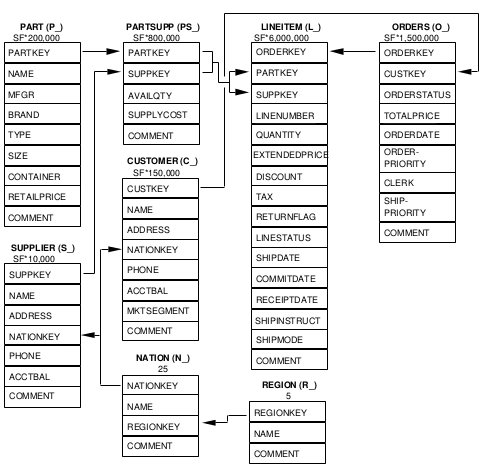
\includegraphics[scale=.6]{TPC-H-Schema}
\caption{TPC-H Schema \cite{TPC-H}}
\label{fig:TPC-H-Schema}
\end{figure}

Der Generator \textit{DBGen} erzeugt die Datenbasis in verschiedenen Größen mit unterschiedlich vielen Tupeln in Abhängigkeit eines Faktors \textit{SF}, der ungefähr der Größe aller Daten in GB entspricht, \textit{SF=1} steht für 1\ GB, die möglichen Größen sind 1\ GB, 10\ GB, 30\ GB, 100\ GB, 300\ GB, 1\ 000\ GB, 3\ 000\ GB, 1\ 0000\ GB, 30\ 000\ GB und 100\ 000\ GB an Daten, die per Zufall erstellt werden.

\begin{figure}[htb]
\centering
\begin{tabular}{p{2,5cm}|p{2,5cm}|p{2,5cm}|p{2,5cm}}
Table Name & Cardinality &  Length (in bytes) &  Typical Table \\\hline
SUPPLIER & 10,000  & 159&  2\\
PART 	& 200,000 &155& 30 \\
PARTSUPP & 800,000 & 144 & 110 \\
CUSTOMER & 150,000 & 179 & 26 \\
ORDERS   & 1,500,000 & 104 & 149 \\
LINEITEM &  6,001,215 & 112 & 641 \\
NATION & 25 & 128 & <1 \\
REGION & 5 & 124 & <1 \\\hline
Total & 8,661,245 && 956
\end{tabular}
\caption{Größe der Relationen bei Faktor SF=1 \cite{TPC-H}}
\end{figure}

\subsection{Implementierung mit Shell-Skripten}
Um nun die Leistungsfähigkeit der Shell-Skripte auf textbasierten Datenbanken zu testen, braucht es drei Werkzeuge: die Daten, die Skripte und natürlich Referenzwerte - die Skripte werden von Hand erzeugt, die Grundlage für die Datenbasis ist dieselbe wie für den TPC-H-Benchmark der Hyper-Schnittstelle\footnote{\url{http://hyper-db.de/interface.html}}, so lassen sich die Ergebnisse auch gut vergleichen.\\

Die Implementierung der SQL-Anfragen orientiert sich an dem vorgestellten Schema im letzten Unterkapitel, nachfolgend sei nur die vierte TPC-H-Anfrage vorgestellt, die Implementierungen der anderen erfolgen analog und sind im Anhang einzusehen. Die vierte Abfrage der Benchmark bewirkt Folgendes:

\begin{quotation}
"`Mit Hilfe dieser Anfrage soll überprüft werden, wie gut das Auftragsprioritätensystem funktioniert. Zusätzlich liefert sie eine Einschätzung über die Zufriedenstellung der Kunden. Dazu zählt die Anfrage die Aufträge im dritten Quartal 1993, bei denen wenigstens eine Auftragsposition nach dem zugesagten Liefertermin zugestellt wurde. Die Ausgabeliste soll die Anzahl dieser Aufträge je Priorität sortiert in aufsteigender Reihenfolge enthalten."' \cite[S. 717]{Kemper}
\end{quotation}


In SQL ausgedrückt sieht das so aus:

\begin{lstlisting}[language=SQL]
select
        o_orderpriority,
        count(*) as order_count
from
        orders
where
        o_orderdate >= date '1993-07-01'
        and o_orderdate < date '1993-10-01'
        and exists (
                select
                        *
                from
                        lineitem
                where
                        l_orderkey = o_orderkey
                        and l_commitdate < l_receiptdate
        )
group by
        o_orderpriority
order by
        o_orderpriority
\end{lstlisting}

Um die Anfragen in Skripte zu übersetzen, hilft die Orientierung am Abfrageplan (siehe Abb. \ref{fig:Queryplan4}). So erhält man einerseits den Ausdruck der relationalen Algebra dafür und eine Schritt-für-Schritt-Übersetzung ist möglich. Außerdem sind so die Ergebnisse besser vergleichbar. Die Tabellen liegen als CSV-Dateien mit Trennzeichen '|' in <tabellenname>.tbl vor, die Kopfzeilen analog in <tabellenname>.csv.

In diesem Fall müssen zuerst die Tabelle \textit{orders} und \textit{lineitem} nach den entsprechenden Tupeln gefiltert werden (o\_orderdate >= date '1993-07-01' and o\_orderdate < date '1993-10-01' und l\_commitdate < l\_receiptdate), in der Shell geschieht dies durch Auswahl der Zeilen mittels \textit{awk}.

\begin{lstlisting}[language=Bash]
sort -k1,1 -t\| orders.tbl | cat orders.csv - | awk -F\| '
        NR==1 || $5<"1993-10-01" && $5>="1993-07-01"{
                print $1"|" $6
        }
' > tmporder.csv

sort -k1,1 -t\| lineitem.tbl |cat lineitem.csv - | awk -F\| '
        NR==1 || $12<$13{
                print $1
        }
' | uniq  |\
\end{lstlisting}

Das anschließende \textit{exists} in SQL wird durch einen linken äußeren Join verwirklicht. Im Gegensatz zu einem Join soll nur auf Existenz überprüft werden, deshalb hilft das Unix-Kommando \textit{uniq} aus, um Duplikate zu eliminieren. 

\begin{lstlisting}[language=Bash]
join --header -t\| -1 1 -2 1 tmporder.csv - > tmp.csv
\end{lstlisting}

Im nächsten Schritt folgt die Gruppierung (\textit{group by}) auf die Spalte \textit{o\_orderpriority}, die einfach durch \textit{uniq} erfolgen kann, bei komplizierteren Aggregatsfunktionen (min, max, sum, count) ist es oft einfacher mit \textit{awk} zu hantieren.

\begin{lstlisting}[language=Bash]
head -1 tmp.csv > tmp1.csv
tail -n+2 tmp.csv  | sort -t\| -k2,2 | cat tmp1.csv - | awk -F\| '
        NR==1{print $2,"order_count"}
        NR==2{g2=$2; count=1}
        NR>2{
                if( g2==$2 ){
                        count++
                }else{
                        print g2, count;
                        g2=$2;count=1;
                }
        }
        END{print g2,count}
' OFS=\|
\end{lstlisting}

Für den Fall der vierten TPC-H-Abfrage kann aber auch \textit{uniq -c} benutzt werden, der neben der Gruppierung auch die Anzahl der Vorkommnisse aller Tupel mit ausgibt, dafür müssen wir uns zunächst auf die relevanten Spalten beschränken (mit \textit{cut}) und alle Zeilen auch sortieren, damit der letztere Befehl ordentlich funktioniert.

\begin{lstlisting}[language=Bash]
cut -d\| -f2 | tail -n+2 | sort | uniq -c
\end{lstlisting}

Und schon ist das Skript fertig, beide Versionen liefern die gewünschte Ausgabe:\\

{\centering \parbox{7cm}{
o\_orderpriority|order\_count\\
1-URGENT|10594\\
2-HIGH|10476\\
3-MEDIUM|10410\\
4-NOT SPECIFIED|10556\\
5-LOW|10487\\
}}
{\parbox{7cm}{
10594 1-URGENT\\
10476 2-HIGH\\
10410 3-MEDIUM\\
10556 4-NOT SPECIFIED\\
10487 5-LOW\\
}}

Die Implementierung aller weiteren TPC-H-Abfragen erfolgte analog. Die Abfragen wurden bei SF=1 und SF=10 getestet. Diese und alle nachfolgenden Läufe wurden auf einem Intel Core i7-3517U mit zwei Kernen (1.90GHz) getestet, die Läufe bei SF=10 erfolgten auf ScyPer-15 mit 40 Kernen.

\begin{figure}[h]
%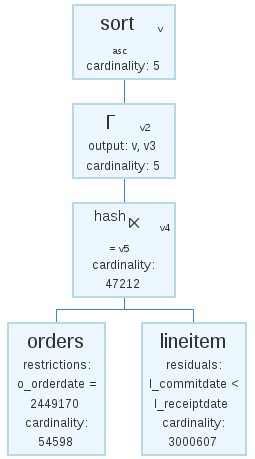
\includegraphics[scale=.6]{Queryplan4}
\Tree [.sort [.$\gamma_{\$2, count(*)}$ [.$\ltimes_{orders.\$1=lineitem.\$1}$
[.$\sigma_{\$5<1993-10-01 \wedge \$5>=1993-07-01}$ orders ]
[.$\sigma_{\$12<\$13}$ lineitem ]
] ] ]
\caption{Abfrageplan zu Nummer 4}
\label{fig:Queryplan4}
\end{figure}

\begin{tikzpicture}
\begin{axis}[
xtick=data,
title=Abfragedauer bei SF1,
scale=1.8,
xlabel={$Abfrage Nr.$},
ylabel={$Zeit [s]$},
]
\addplot[
ybar,
fill = blue,
color = blue
] coordinates {
(1,47.420)
(2,6.372)
(3,32.022)
(4,22.544)
(5,26.827)
(6,7.949)
(7,18.713)
(8,39.677)
(9,54.243)
(10,12.971)
(11,2.934)
(12,22.859)
(13,7.068)
(14,7.185)
(15,29.784)
(16,4.957)
(17,37.156)
(18,25.484)
(19,6.728)
(20,58.405)
(21,63.225)
(22,6.178)
};

%\addplot[
%color=green,
%mark = *,
%only marks
%] coordinates{
%(3,29.276)
%(5,24.441)
%(7,17.680)
%(9,46.270)
%};
%\legend{nach Abfrageplan, Bash-optimierter Abfrageplan}
\end{axis}
\end{tikzpicture}

\begin{tikzpicture}
\begin{axis}[
xtick=data,
title=Abfragedauer bei SF10,
scale=1.8,
xlabel={$Abfrage Nr.$},
ylabel={$Zeit [s]$},
]
\addplot[
ybar,
fill = blue,
color = blue
] coordinates {
(1,	572.857)
(2,	73.534)
(3,	443.247)
(4,	234.677)
(4,	238.975)
(5,	307.112)
(6,	140.614)
(7,	260.438)
(8,	518.944)
(9,	304.204)
(10,	195.974)
(11,	34.194)
(12,	261.685)
(13,	100.206)
(14,	128.932)
(15,	446.731)
(16,	66.396)
(17,	468.63)
(18,	320.389)
(19,	175.907)
(20,	806.291)
(21,	891.314)
(22,	82.748)
};
\end{axis}
\end{tikzpicture}

\subsection{Optimierung durch Parallelisierung}
Ein kurzer Blick auf die laufenden Prozesse bestätigt einen Verdacht: die Abfragen laufen teils parallel, es werden so viele Prozesse gestartet wie Kommandos in einer Pipeline verwendet. Von den meisten heutigen Bash-Philosophen wird dies verschwiegen, daher lohnt sich ein Blick in das Buch von Pike und des awk-Erfinders Kernighan.

\begin{figure}[h]
\centering
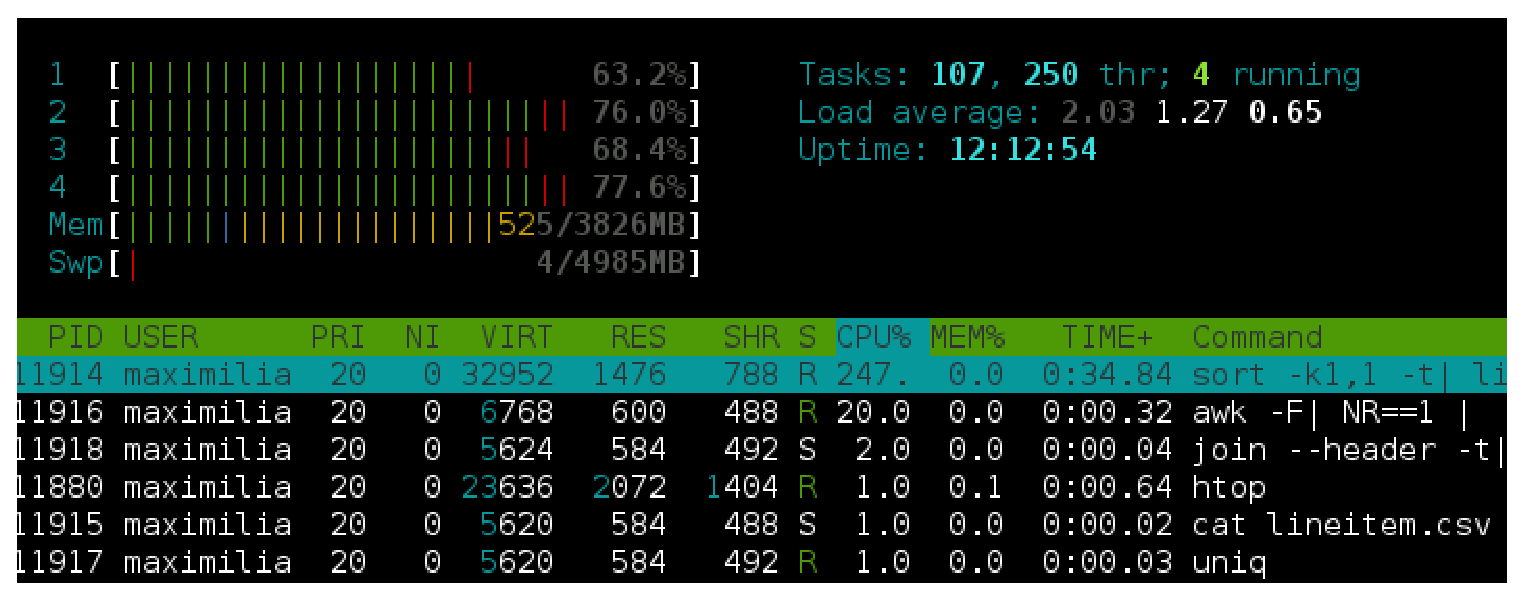
\includegraphics[scale=.5]{htop.eps}
\caption{Parallele Ausführung mittels Pipe verbundener Prozesse}
\label{fig:htop}
\end{figure}

\begin{quote}
"`Die Programme in der Pipeline werden in Wirklichkeit gleichzeitig ausgeführt, nicht nacheinander. Das bedeutet, da[ss] die Programme in einer Pipeline interaktiv arbeiten können; der Betriebssystem-Kern sorgt für die nötige Zuteilung von Rechenzeit und Synchronisation, damit alles funktioniert."' \cite[S. 34]{TUPE}
\end{quote}

Das Ziel ist es also, eine möglichst hohe Druchlaufquote durch die Verwendung von Pipelines zu erzielen. Jedoch geht dies nur bis zu einem gewissen Grad, die zwangsweise Sortierung der Datenbestände vor Joins macht die Aufteilung in einen Kopf und einen Rumpf erforderlich, der Kopf bleibt unverändert, der Rumpf wird sortiert und alles in eine Datei umgeleitet oder mit \textit{cat} wieder zusammengefügt.

\begin{lstlisting}[language=Bash]
head -1   tmprns.csv > tmp1.csv
tail -n+2 tmprns.csv | sort -t\| -k2,2 >> tmp1.csv
head -1   join5.csv > tmp2.csv
tail -n+2 join5.csv | sort -t\| -k2,2 | cat tmp2.csv - |\
join --header -t\| -1 2 -2 2 tmp1.csv - |\
\end{lstlisting}

Versuche, die Kommandos in eine Pipeline zu packen, schlagen kläglich fehl. Jetzt wäre es doch praktisch, ein alternatives Konstrukt zu nutzen, sodass die Verarbeitung parallel ablaufen kann. Benannte Pipes sind die Lösung, sie können einfach erstellt werden.

\begin{lstlisting}[language=Bash]
$ mkfifo mypipe
\end{lstlisting}

Wichtig ist, dass die Prozesse, die in die Pipe hineinschreiben und aus ihr herauslesen, parallel ablaufen. Die Pipe blockiert so lange, bis aus ihr gelesen, bzw. in sie geschrieben worden ist.

Nachfolgend ein einfaches Beispiel, das bereits 13\% Zeit einspart und zeitlich fast an eine Pipeline herankommt.\\
\lstinline{$ sort orders.tbl | grep final} benötigt 2,752 s\\
Ohne die Pipeline können die Prozesse über eine Datei kommunizieren oder über eine benannte Pipe:\\

{\footnotesize \texttt{ \parbox{7cm}{
%\begin{lstlisting}[language=Bash]
\#!/bin/bash\\
sort \$1 > tmpfile\\
grep final < tmpfile\\
%\end{lstlisting}
}
\parbox{7cm}{
%\begin{lstlisting}[language=Bash]
\#!/bin/bash\\
mkfifo mypipe\\
(sort \$1 > mypipe)\&\\
grep final < mypipe
%\end{lstlisting}
}}}\\


Mit Umlenkung in eine Datei werden 3,165 s gebraucht, die zweite Variante schlägt die erste mit nur 2,760 s und liegt damit dicht an einer Pipeline.
%real	0m2.752s
%user	0m7.620s
%sys	0m0.212s
%real	0m2.760s
%user	0m7.644s
%sys	0m0.212s
%real	0m3.165s
%user	0m7.488s
%sys	0m0.288s
Darüberhinaus ist es von Vorteil, dass ein Prozess im Hintergrund und somit auch parallel läuft. Und synchronisiert sind sie auch, sie müssen nicht explizit auf ihren Vorgängerprozess warten. Solange in die Pipe noch nicht geschrieben ist, wird der andere Prozess blockiert. Lediglich die Reihenfolge ist wichtig. Auf diese Weise werden die TPC-H-Anfragen nun optimiert: Zuerst wird die Kopfzeile geschrieben, dann der Rumpf.
\begin{lstlisting}[language=Bash]
head -1   tmprns.csv > tmp.csv &
tail -n+2 tmprns.csv | sort -t\| -k2,2 | cat tmp.csv - > tmp1.csv &
head -1   join5.csv > tmp2.csv &
tail -n+2 join5.csv | sort -t\| -k2,2 | cat tmp2.csv - |\
join --header -t\| -1 2 -2 2 tmp1.csv -
\end{lstlisting}

Analog dazu werden nun alle Anfragen optimiert und die neue Zeit gemessen.

\begin{tikzpicture}
\begin{axis}[
xtick=data,
legend style={at={(0.5,0.97)},
         anchor=north,legend columns=-1},
title=Abfragedauer bei SF1,
ybar = 0.25pt,
width=0.95\textwidth,height=0.48\textheight,
bar width=6pt,
xlabel={$Abfrage Nr.$},
ylabel={$Zeit [s]$},
]
\addplot[
ybar,
fill = blue,
] coordinates {
(1,47.420)
(2,6.372)
(3,32.022)
(4,22.544)
(5,26.827)
(6,7.949)
(7,18.713)
(8,39.677)
(9,54.243)
(10,12.971)
(11,2.934)
(12,22.859)
(13,7.068)
(14,7.185)
(15,29.784)
(16,4.957)
(17,37.156)
(18,25.484)
(19,6.728)
(20,58.405)
(21,63.225)
(22,6.178)
};
\addplot[
ybar,
fill=orange,
] coordinates{
(2,5.974)
(3,31.000)
(4,22.466)
(5,24.696)
(7,18.294)
(8,37.294)
(9,52.910)
(10,12.374)
(11,2.906)
(12,21.855)
(13,6.271)
(14,6.767)
(15,29.505)
(16,4.354)
(17,37.317)
(18,24.947)
(19,6.443)
(20,59.412)
(21,46.289)
(22,5.921)
};
\legend{original,optimiert}
\end{axis}
\end{tikzpicture}

\begin{tikzpicture}
\begin{axis}[
xtick=data,
legend style={at={(0.5,0.97)},
         anchor=north,legend columns=-1},
title=Abfragedauer bei SF10,
width=0.95\textwidth,height=0.48\textheight,
ybar = 0.25pt,
bar width=6pt,
xlabel={$Abfrage Nr.$},
ylabel={$Zeit [s]$},
]
\addplot[
ybar,
fill = blue,
] coordinates {
(1,	572.857)
(2,	73.534)
(3,	443.247)
(4,	234.677)
(4,	238.975)
(5,	307.112)
(6,	140.614)
(7,	260.438)
(8,	518.944)
(9,	304.204)
(10,	195.974)
(11,	34.194)
(12,	261.685)
(13,	100.206)
(14,	128.932)
(15,	446.731)
(16,	66.396)
(17,	468.63)
(18,	320.389)
(19,	175.907)
(20,	806.291)
(21,	891.314)
(22,	82.748)
};

\addplot[
ybar,
fill = orange,
] coordinates{
(2,	73.534)
(3,	443.247)
(5,	305.788)
(7,	254.706)
(8,	492.842)
(9,	277.647)
(10,	189.187)
(11,	34.22)
(12,	222.58)
(13,	90.957)
(14,	122.453)
(16,	56.808)
(17,	472.637)
(18,	308.145)
(19,	172.96)
(20,	812.589)
(21,	642.894)
(22,	77.706)
};
\legend{original,optimiert}
\end{axis}
\end{tikzpicture}

Bei fast allen Abfragen konnten leichte Verbesserungen erzielt werden, bei den meisten zwar nur unerheblich, aber bei der vorletzten Abfrage ist deutlich zu sehen, was ein bisschen Parallelisierung bewirkt, sie läuft um 28\ \% schneller.
Eine weitere Möglichkeit Parallelität zu erreichen ist die Prozesse mit \textit{split} aufzuteilen. Dieser Befehl erzeugt aus einer Datei mehrere kleine aufsteigend benannte Dateien (beginnend bei \textit{aa} bis \textit{zz}, auch mit benannten Pipes kompatibel), auf denen die Anfragen laufen. Das Zusammenfügen passiert am Ende mit \textit{cat}. Bei kleinen Anfragen dauert das Teilen länger als was die Parallelität einspart.

\begin{lstlisting}[language=Bash]
$ grep final lineitem.tbl
\end{lstlisting}
Das Skript nun mit geteilter Quelldatei und Ausführung der Prozesse im Hintergrund.
\begin{lstlisting}[language=Bash]
#!/bin/bash
mkfifo mini.aa mini.ab g1 g2
(split -n2 lineitem.tbl mini.)&
(grep final mini.aa > g1)&
(grep final mini.ab > g2)&
cat g1 g2

rm mini* g1 g2
\end{lstlisting}
Das Skript verdeutlicht die Parallelität durch Teilen, die getestete Ausführung benötigt jedoch 0,2\ s länger (2,8\ s statt 2,6\ s).\\

Komplizierter wird die Syntax, wenn die Parallelisierung über GNU Parallel läuft. Dieses bietet zahlreiche Funktionen an, die aber über den Inhalt dieses Kapitels - einfache Skripte wie sie in der Wissenschaft vorkommen zu erstellen - hinaus gehen. Zusammen mit nachfolgendem Beispiel sei aber auf die Literatur verwiesen \cite{DataScience}.
\begin{lstlisting}[language=Bash]
$ seq 4 | parallel "echo {}"
1
2
3
4
\end{lstlisting}

		
		%\part[Vergleich]{Vergleich existierender Tools für textbasierte Datenbanken}
		%\label{part:secondP}
		\chapter{Vergleich}
Welche Ansätze existieren bereits, um Abfragen an CSV-Dateien auszuführen? Grob lassen sich diese in zwei Kategorien unterteilen: Programme, die mit ihrer eigenen Syntax SQL-ähnliche Funktionen imitieren, und solche, die SQL-Abfragen ohne Datenbank auf Textdateien ausführen.

\section{SQL-ähnliche Syntax}
\subsection{Datamash}
Ein wunderbares Programm für die Analyse auf Textdateien ist \textit{datamash},
\footnote{\url{http://www.gnu.org/software/datamash/}}
das numerische Operationen auf Datensätze ausführen kann und dabei auch die meisten Operationen des $\gamma$-Operators beherrscht. Das Programm ist in C geschrieben, arbeitet ausschließlich als Filter für DSV-Dateien (Trennzeichen standardmäßig Tab) und erwartet in den Optionen die Spalten nach denen gruppiert wird und als Argument die auszuführende Aktion.
\begin{lstlisting}[language=Bash]
$ cat myexample
A	1
A	3
B	2
$ cat myexample | datamash sum 2
6
$ datamash -g1 sum 2
A	4
B	2
\end{lstlisting}

Um das Programm in die Skripte der TPC-H-Abfragen einzubinden, soll es Kopfzeilen erkennen und das Trennzeichen muss variabel bestimmt werden. Beides kann datamash, die Option \textit{--headers} oder \textit{-H} weist die erste Zeile als Kopf aus und mit \textit{--field-separator=,} oder \textit{-t,} wird das Komma ',' als Separator bestimmt.
\begin{lstlisting}[language=Bash]
$ cat myexample
Name,Zahlen
A,1
A,3
B,2
$ datamash -H -t, -g1  sum 2
Name,sum(Zahlen)
A,4
B,2
\end{lstlisting}

Sieht das Gruppieren und anschließende Summieren, Zählen, Mittelwertbilden kompliziert aus, so dient jetzt eine einzige Anfrage dazu, die Option \textit{-s} erspart einem sogar das vorherige Sortieren, nachfolgend die angepasste erste TPC-H Abfrage (erste Berechnung weiterhin mit awk).

\begin{lstlisting}[language=Bash]
#!/bin/bash
#2014-09-01
cat lineitem.* | awk -F\| '
        NR==1{
                print $0 "sum_disc|sum_charge|"
        }
        NR>1 && $11<="1998-9-2"{
                suma=($6*(1.0-$7));
                sumb=($6*(1.0-$7)*(1.0+$8));
                print $0 suma "|" sumb "|"
        }
' > tmp.csv
head -1 tmp.csv > tmp1.csv
tail -n+2 tmp.csv | sort -t\| -k9,10 | cat tmp1.csv - |\
datamash -t\| -H -g9,10 sum 5 sum 6 sum 17 sum 18 mean 5 mean 6 mean 7 count 1
\end{lstlisting}

Zu beachten ist, dass datamash Dezimalzahlen im länderspezifischen Format ausgibt und auch solche in der Eingabe benötigt. Sind die Datensätze auf ein anderes Format ausgelegt, so sind meist '.' und ',' ganz einfach durch den Befehl \textit{tr} zu vertauschen.
\begin{lstlisting}[language=Bash]
$ cat datei |  tr '.,' ',.'
\end{lstlisting}

Auf diese Weise werden die Skripte mit datamash geschrieben und auch wieder die Zeit gemessen.

%\begin{figure}[b]
\begin{tikzpicture}
\begin{axis}[
xtick=data,
legend style={at={(0.5,0.97)},
         anchor=north,legend columns=-1},
title=Abfragedauer bei SF1,
width=0.95\textwidth,height=0.48\textheight,
ybar = 0.25pt,
bar width=6pt,
xlabel={$Abfrage Nr.$},
ylabel={$Zeit [s]$},
]
\addplot[
ybar,
fill = blue,
] plot coordinates {
(1,47.420)
(2,6.372)
(3,32.022)
(4,22.544)
(5,26.827)
(6,7.949)
(7,18.713)
(8,39.677)
(9,54.243)
(10,12.971)
(11,2.934)
(12,22.859)
(13,7.068)
(14,7.185)
(15,29.784)
(16,4.957)
(17,37.156)
(18,25.484)
(19,6.728)
(20,58.405)
(21,63.225)
(22,6.178)
};
\addplot[
ybar,
fill  = orange
] plot coordinates{
%datamash
(1,61.962)
(2,6.494)
(3,28.086)
(4,22.332)
(5,37.344)
(6,8.024)
(7,23.258)
(8,24.036)
(9,45.607)
(10,15.708)
(11,3.037)
(12,23.359)
(13,7.992)
(14,8.099)
(15,7.581)
(16,3.532)
(17,48.223)
(18,18.802)
(19,8.611)
(20,11.221)
(21,43.384)
(22,6.565)
};
\legend{Abfragen nur mit awk, Abfragen mit datamash}
\end{axis}
\end{tikzpicture}
%\end{figure}

In den meisten Fällen sind die umgeschriebenen Skripte langsamer, in manchen aber auch deutlich schneller. Der Vorteil an den Skripten, die ausschließlich awk nutzen, ist, dass Berechnungen und das Gruppieren in einem Schritt erfolgen kann. datamash unterstützt nur Aggregatsfunktionen und keine arithmetischen Ausdrücke, sodass für Berechnungen ein weiteres Programm benötigt wird. Der Vorteil von datamash liegt aber in der Einfachheit, mit der Aggregatsfunktionen eingegeben werden können.
Auf der Seite zu datamash sind auch äquivalente Kommandos mit anderen Programmen aufgelistet.
\footnote{\url{http://www.gnu.org/software/datamash/alternatives/}}\\\\
Fazit: datamash ist ein sehr schönes Programm, das einem die Arbeit erleichtern kann, der kompliziertere Umgang mit awk kann aber zu schnelleren Abfragen führen.

\subsection{csvtool}
Das in OCaml geschriebene csvtool ist mittlerweile in allen Linux-Pa\-ket\-ver\-wal\-tungs\-sys\-te\-men erhältlich und richtet sich an Nutzer mit komplizierteren CSV-Datensätzen.
\footnote{\url{https://forge.ocamlcore.org/projects/csv/}}
Im Grunde ersetzt das csvtool die klassischen Unix-Werkeuge wie grep, cut, head, tail, join, wc -l, usw., jedoch kann es auch problemlos mit Spezialfällen hantieren, in denen sich ein Datensatz über mehrere Zeilen erstreckt.
Die Selektion heißt dort \textit{namedcol}.
\begin{lstlisting}[language=Bash]
$ csvtool namedcol ID,Name Punktetabelle.csv 
1,Franz
2,Alfred
3,Marie
\end{lstlisting}

Für Joins ist csvtool nur bedingt geeignet, die Syntax ist alles andere als intuitiv.
\begin{lstlisting}[language=Bash]
$ csvtool join <Joinattribute> <Tabellennummer> Tabelle1 Tabelle2
\end{lstlisting}

Bei Joinattribute werden beginnend bei 0 die zu vergleichenden Spalten eingetragen, bei Tabellennummer als Liste die Spalten, die später sichtbar sein sollen. Dabei bezieht sich die Auswahl aber immer auf beide Tabellen, folglich müssen Joinattribute an der gleichen Position stehen.

\begin{lstlisting}[language=Bash]
$ csvtool join 1 2,3 Punktetabelle.csv Zeittabelle.csv 
1,Franz,50,44,
2,Alfred,10,88,
3,Marie,27,67,
ID,Name,Punkte,Zeit,
\end{lstlisting}

Für relationale Algebra ist das Programm weniger gedacht als für einfach Vergleiche von CSV-Datensätzen. Für komplizierte Abfragen empfehlen sich mächtigere Programme, die in den meisten Fällen auch SQL-Ausdrücke beherrschen und deshalb noch vorgestellt werden.

\subsection{Fsdb}
Seit 1991 existiert Fsdb als eine textdateibasierte Datenbank (flat text database for shell scripting), die jedoch ihrem eigenen Datenformat gehorcht und Operationen ähnlich zu datamash beherrscht.
\footnote{\url{http://www.isi.edu/~johnh/SOFTWARE/FSDB/}}

Die Textdateien enden auf \textit{.fsdb}, am Anfang steht eine Kopfzeile, gekennzeichnet durch "'\#fsdb"', mit den Spaltenbezeichnern, anschließend die durch Leerräume separierten Werte.
Das Feldtrennzeichen kann mit \textit{-F} verändert werden, Kommentare beginnen mit '\#', mit dem Befehl \textbf{csv\_to\_db} können CSV-Dateien in das Format konvertiert werden.

\begin{lstlisting}
$ cat Punktetabelle.fsdb
#ID Name Punkte
1 Franz 50
2 Alfred 10
3 Marie 27
$ cat Punktetabelle.fsdb | dbcol ID Name Punkte
#fsdb ID Name Punkte
1	Franz	50
2	Alfred	10
3	Marie	27
\end{lstlisting}

Die Kommandos von Fsdb arbeiten als Filter, sie lesen also von der Standardeingabe Daten ein, die immer im entsprechenden Format stehen müssen. Insgesamt eine nette Idee, das Erlernen der vielen verschiedenen Kommandos nur eher unintuitiv.

\section{Abfragen mit SQL}

\begin{figure}
\centering
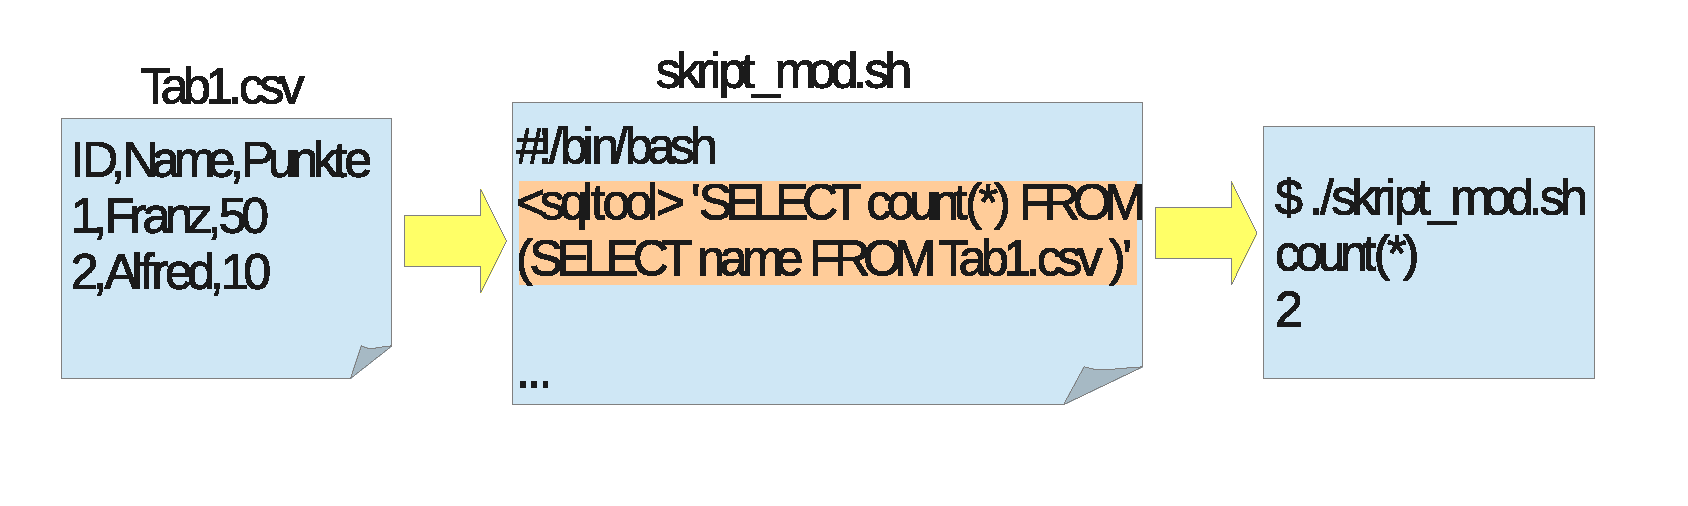
\includegraphics[scale=.4]{vergleich.eps}
\caption{Funktionsweise von SQL-Tools in der Kommandozeile}
\label{fig:vergleich}
\end{figure}

\subsection{txt-sushi}
Ein geniale Sammlung von Programmen, um auf CSV-Dateien mit SQL-Syntax zuzugreifen ist \textbf{txt-sushi}. Einmal installiert, so bietet es neben zahlreichen weiteren Funktionen, die die Ausgabe von Textdateien verschönern, auch ein Programm \textbf{tssql} an, mit dem sich in SQL formulierte Abfragen auf CSV-Dateien ausführen lassen.
\footnote{\url{http://keithsheppard.name/txt-sushi/}}

\begin{lstlisting}[language=Bash]
$ tssql 'select * from `orders.csv`'
O_Id,OrderDate,OrderPrice,Customer
1,2008/11/12,1000,Hansen
2,2008/10/23,1600,Nilsen
3,2008/09/02,700,Hansen
4,2008/09/03,300,Hansen
5,2008/08/30,2000,Jensen
6,2008/10/04,100,Nilsen
\end{lstlisting}
Das Programm arbeitet auch als Filter und kann von der Standardausgabe lesen, die Daten können über eine Pipe weitergereicht werden. Generell gilt, alle Daten, die eingelesen werden sollen, werden mit zwei Gravis (back tick, ' ` ') geklammert.
\begin{lstlisting}[language=Bash]
$ cat orders.csv | tssql 'select * from `-`'
O_Id,OrderDate,OrderPrice,Customer
1,2008/11/12,1000,Hansen
2,2008/10/23,1600,Nilsen
...
\end{lstlisting}

Noch einfacher können die Tabellen gleich über Optionen eingebunden werden, dort werden auch Bezeichner für die Dateien definiert.
\begin{lstlisting}[language=Bash]
$ tssql -table orders orders.csv 'select * from orders'
\end{lstlisting}

Leider akzeptiert das Programm nur durch Komma separierte Dateien, wird ein anderes Symbol als Trennzeichen verwendet, so muss das über eine Umlenkung erfolgen.
\begin{lstlisting}[language=Bash]
$ tssql -table orders <(sed 's/;/,/g' orders_mit_Semikolon.csv) 'select * from orders'
\end{lstlisting}
Probleme bereitet dies, wenn Kommata Bestandteil der Datensätze sind. Am einfachsten ist es, den Programmcode so umzuschreiben, sodass ein anderes Zeichen die Daten voneinander trennt. (Die Quelldateien finden sich auf Github, zu verändern ist die Datei \textit{txt-sushi-master/Database/TxtSushi/FlatFile.hs})
\footnote{\url{https://github.com/keithshep/txt-sushi}}

So kann auch ein einfaches Skript geschrieben werden, um größere SQL-Abfragen gemäß dem TPC-H Schema einzugeben.
\begin{lstlisting}[language=Bash]
#!/bin/bash
TSSQL=/home/maximilian/Downloads/txt-sushi-master/tssql
$TSSQL -table lineitem <(cat lineitem.*) '
SELECT
        l_returnflag,
        l_linestatus
FROM
        lineitem
GROUP BY
        l_returnflag,
        l_linestatus
'

\end{lstlisting}
Bei der Ausführung selbst einfacher Abfragen wie der gerade beschriebenen stellt man schnell fest, dass der Arbeitsspeicher den limitierenden Faktor darstellt. Sobald größere Operationen durchgeführt werden, die über eine Selektion hinausgehen, so lädt das Haskell-Programm alle Datensätze in den Hauptspeicher. Das beschriebene Skript wird nach einiger Zeit durch das System beendet. Für große Datenmengen ist das Programm nicht geeignet, obwohl es in der Bedienung und von der Funktion einzigartig gut und praktisch ist.

\subsection{csvfix}
Die meisten Datenbanksysteme unterstützen den Import von CSV-Dateien, aber leider nicht alle. Besonders im mobilen Bereich, wo Anwender auf gewisse Datenbanken nur über eine SQL-Schnittstelle zugreifen können, sind SQL-Anweisungen zum Einfügen von Daten von Vorteil (s. Abb. \ref{fig:konvert}). Dagegen hilft csvfix, das aus gegebenen CSV-Datensätze entsprechend viele INSERT-/UPDATE/- oder DELETE-Anweisungen generiert. Einfach den Tabellennamen, die Spaltenbezeichner und die Quelldatei angeben, schon werden die SQL-Anweisungen erzeugt, mit der Option \textit{-ifn} wird die erste Zeile als Kopfzeile betrachtet.
\begin{lstlisting}[language=Bash]
$ cat Punktetabelle.csv
ID,Name,Punkte
1,Franz,50
2,Alfred,10
3,Marie,27
$ csvfix sql_insert -ifn -t punktetabelle -f 1:ID,2:Name,3:Punkte Punktetabelle.csv
INSERT INTO punktetabelle ( ID, Name, Punkte ) VALUES( '1', 'Franz', '50');
INSERT INTO punktetabelle ( ID, Name, Punkte ) VALUES( '2', 'Alfred', '10');
INSERT INTO punktetabelle ( ID, Name, Punkte ) VALUES( '3', 'Marie', '27');
\end{lstlisting}

Über die Option \textit{-sep} kann noch das Feldtrennzeichen angegeben werden, sollen Felder ohne Anführungszeichen ausgegeben werden, so dient die Option \textit{-nq} dazu.
\begin{lstlisting}[language=Bash]
$ csvfix sql_insert -ifn -sep , -t punktetabelle -nq 1,3 -f 1:ID,2:Name,3:Punkte Punktetabelle.csv
INSERT INTO punktetabelle ( ID, Name, Punkte ) VALUES( 1, 'Franz', 50);
INSERT INTO punktetabelle ( ID, Name, Punkte ) VALUES( 2, 'Alfred', 10);
INSERT INTO punktetabelle ( ID, Name, Punkte ) VALUES( 3, 'Marie', 27);
\end{lstlisting}

\begin{figure}
\centering
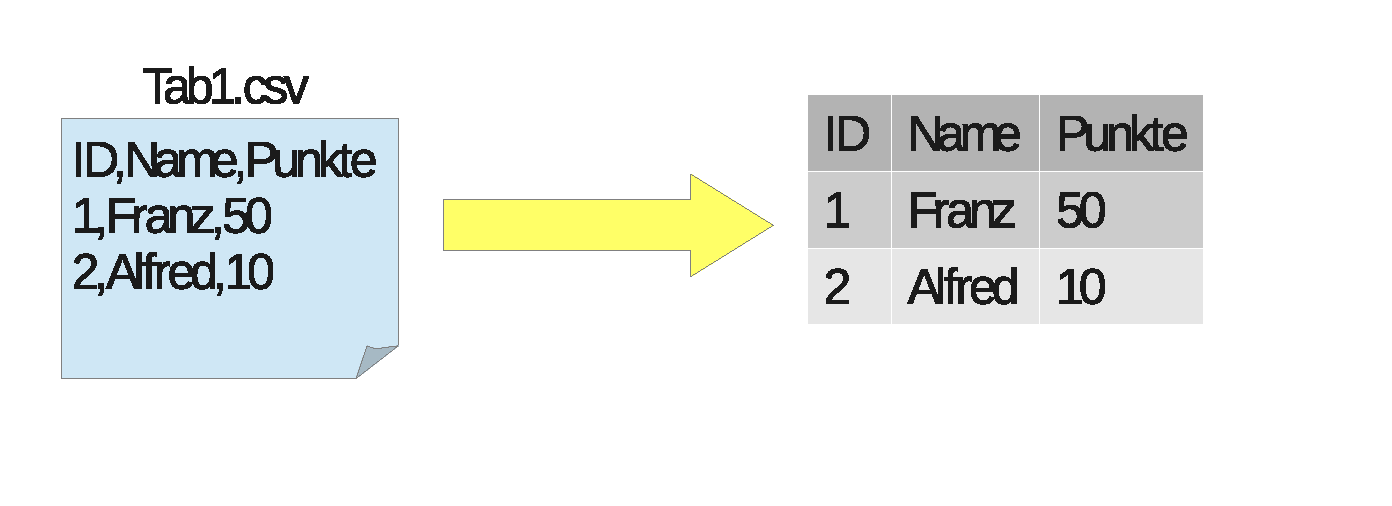
\includegraphics[scale=0.4]{konvert.eps}
\caption{Import von CSV}
\label{fig:konvert}
\end{figure}

Doch csvfix kann mehr, als nur SQL-Befehle generieren, ähnlich dem csvtool unterstützt es auch den Verbund mehrerer Tabellen und weitere arithmetische Operationen ähnlich zu awk.
\footnote{\url{http://csvfix.byethost5.com/csvfix15/csvfix.html}}
\begin{lstlisting}[language=Bash]
$ csvfix join -f 1:1 Zeittabelle.csv Punktetabelle.csv 
"ID","Zeit","Name","Punkte"
"1","44","Franz","50"
"2","88","Alfred","10"
"3","67","Marie","27"
\end{lstlisting}
Äquivalenzen werden durch den Doppelpunkt beschrieben (\textit{Feld von i : Feld von i+1}), in einem Schritt können mehrere Joins vollzogen werden, es werden einfach mehrere Quelldateien angegeben.

Generell gibt es für die meisten benötigten Kommandos ein Äquivalent in csvfix, der Vorteil liegt an den unterstützten Standards, ein Komma als Feldinhalt stellt kein Problem dar. Abgesehen von diesen Spezialfällen reichen auch die klassischen Kommandos aus.

\subsection{csvkit}
Die Funktionen von csvfix und txt-sushi kombiniert bietet das von der Literatur gepriesene csvkit \cite{DataScience}. Es unterstützt zwar auch einfache Operationen um CSV-Dateien auszugeben, ist aber primär auf das Anwenden von SQL-Abfragen auf CSV-Dateien ausgelegt und bietet an, bei größeren Datenmengen die Abfrage über eine Datenbankverbindung auszuführen.
\footnote{\url{https://csvkit.readthedocs.org/en/latest/index.html}}

Zuerst einmal ist es fähig, eine Anweisung zum Erstellen von Datenbank-Schemata auszugeben und erkennt dabei selbständig den Typ. Über die Option \textit{-i} ist die Anweisung sogar auf bestimmte Datenbanktypen zugeschnitten.
\begin{lstlisting}[language=Bash]
$ csvsql -i postgresql Punktetabelle.csv
CREATE TABLE "Punktetabelle" (
	"ID" INTEGER NOT NULL, 
	"Name" VARCHAR(6) NOT NULL, 
	"Punkte" INTEGER NOT NULL
);
\end{lstlisting}

Leider kann das Programm keine Operationen zum Einfügen direkt generieren, dafür dient csvfix. Stattdessen ist es möglich, über eine Datenbankanbindung direkt die CSV-Dateien zu importieren.

\begin{lstlisting}[language=Bash]
$ csvsql --db <Verbindung zur Datenbank> --insert Punktetabelle.csv
\end{lstlisting}

Aber nun folgt die Option \textit{--query}, um eine SQL-Anweisung direkt auszuführen, mit \textit{-d} kann auch das Trennzeichen bestimmt werden.

\begin{lstlisting}[language=Bash]
$ csvsql -d, --query 'select * from Punktetabelle' Punktetabelle.csv
ID,Name,Punkte
1,Franz,50
2,Alfred,10
3,Marie,27
\end{lstlisting}

Das Programm arbeitet nur auf CSV-Dateien, die auch eine Kopfzeile besitzen und auf die Dateiendung \textit{.csv} hören, alles andere akzeptiert es nicht, trotz Modifikation können die TPC-H Abfragen aufgrund ihrer Größe nicht ausgeführt werden.

\subsection{querycsv.py}
Das in Python geschriebene Skript querycsv.py arbeitet ähnlich und ist flexibler in der Annahme von Dateinamen.
\footnote{\url{https://pypi.python.org/pypi/querycsv}}

\begin{lstlisting}[language=Bash]
$ alias querycsv='/home/maximilian/Downloads/querycsv-0.3.0.0/querycsv/querycsv.py'
$ querycsv -i Punktetabelle.csv 'Select * From Punktetabelle'
 ID | Name   | Punkte
======================
 1  | Franz  | 50    
 2  | Alfred | 10    
 3  | Marie  | 27  
\end{lstlisting}

Dank eines CSV-Sniffers erkennt das Programm automatisch das Feldtrennzeichen, leider sind die möglichen Trennzeichen dadurch auch beschränkt, eine Pipe '|' zum Trennen wird nicht unterstützt. Ohne Modifikation der CSV-Dateien ist auch dieses Programm für die TPC-H Abfragen nicht zu nutzen.
\begin{lstlisting}[language=Python]
dialect = csv.Sniffer().sniff(open(infilename, "rt").readline())
\end{lstlisting}
Die Endung der Dateien auf \textit{.tbl} erkennt das Skript mühelos, der Name zuvor wird als Tabellenbezeichner verwendet, nur werden keine Daten ohne Kopfzeile akzeptiert, wie auch durch Pipe getrennte Dateien. Liegen die Daten der TPC-H Anfragen in einer Datei, so ist diese zu groß für das Programm. Fazit: Ein sehr schönes Skript, aber Mangel an Flexibilität.

\subsection{gcsvsql}
Ein ähnliches Programm wie csvsql, heißt gcsvsql, da es auf Groovy basiert, einer objektorientierten Skriptsprache und der Name csvsql schon vergeben ist.
\footnote{\url{https://code.google.com/p/gcsvsql/}}
Die Abfrage wird einfach als SQL-Anweisung eingegeben, als Tabelle steht der Name der CSV-Datei.
\begin{lstlisting}[language=Bash]
$ gcsvsql "select * from Punktetabelle.csv"
\end{lstlisting}

Wegen der starren Syntax und einer seltenen Programmiersprache erweist sich die Anwendung des Programms als schwierig.

\subsection{Mynodbcsv}
Einen ähnlichen Ansatz wie txt-sushi nur noch optimierter und einen Schritt weiter geht das Konzept Mynodbcsv, das vor Kurzem veröffentlicht worden ist.
Insgesamt geht es um das Problem, wie sehr große Datenmengen aus CSV-Dateien mit SQL-Anweisungen abgefragt werden, ohne dabei die kompletten Daten in eine Datenbank zu importieren und auch kein Datenbankschema vorher konfigurieren zu müssen.\\
Das Konzept analysiert anhand einer optimierten Abfrage zuerst die relevanten Felder einer CSV-Datei, anschließend lädt es nur die relevanten Daten in eine SQLite-Datenbank, worauf die Abfrage laufen kann. Somit geht dieses Konzept einen Mittelweg, es müssen nie alle Daten in eine Datenbank importiert werden, trotzdem erfolgt die Abfrage mittels eines Datenbanksystems. Für die genauen Messergebnisse sei auf die Veröffentlichung verwiesen \cite{Mynodbcsv}.

\subsection{shql}
Ähnlich der geschriebenen Abfragen als TPC-H Skripte implementiert shql eine Datenbank, die ausschließlich auf den Unix-Kommandos basiert und SQL über awk-Funktionen interpretiert.
\footnote{\url{http://lorance.freeshell.org/shql/}}


		%\part[Parser]{Der Bash zu SQL Parser}
		\chapter{Parser mit Yacc und Lex}
Wie bereits gesehen, Programme, die eine CSV-Datei parsen und diese in SQL importieren, gibt es bereits genügend, genauso wie die Möglichkeit existiert, auf Textdateien SQL-Abfragen laufen zu lassen. Außerdem ist auch analysiert worden, welche Bash-Konstrukte bestimmten SQL-Abfragen entsprechen. Darum nun der abschließende Teil der Arbeit - wie können Shell-Skripte geparst und in SQL übersetzt werden.

\section{Vorwissen zu Yacc und Lex}
Der erste Versuch verwendet Yacc, ein Programm, das Anfang der 1970-er Jahre von Stephen Curtis Johnson unter dem Namen "`yet another compiler compiler"' für den Compilerbau erfunden und im GNU-Projekt durch Bison ersetzt worden ist. Die Grammatik wird in einer Art Backus-Naur-Form eingegeben, der Parsergenerator Yacc erzeugt dann automatisch ein C-Programm, das von einer entsprechenden Eingabe liest \cite{meinders}.

\section{Der Bash2SQL-Übersetzer mit Yacc}
Das Ziel des Bash2SQL-Übersetzer ist zu zeigen, dass der Weg, ein Shell-Skript in eine SQL-Abfrage zu übersetzen, schaffbar ist. Darum behandelt dieser Parser die grundlegende Idee mit vereinfachter Grammatik und fokussiert die korrekte Übersetzung der Befehle.

\subsection{Arbeitsweise}
Wie sollen die Kommandos übersetzt und verbunden werden? Die erste Überlegung kombiniert jeden auftretenden Befehl zu einer SQL-Abfrage, bis es nicht mehr möglich ist,
ein \textit{cat tabelle} füttert den From-Teil, ein über Pipe verbundenes \textit{wc -l} füttert die Select-Klausel desselben Structs mit einem \textit{count(*)}, am Ende wird die Abfrage ausgegeben (s. Abb. \ref{fig:parser1}).

\begin{figure}[h]
\centering
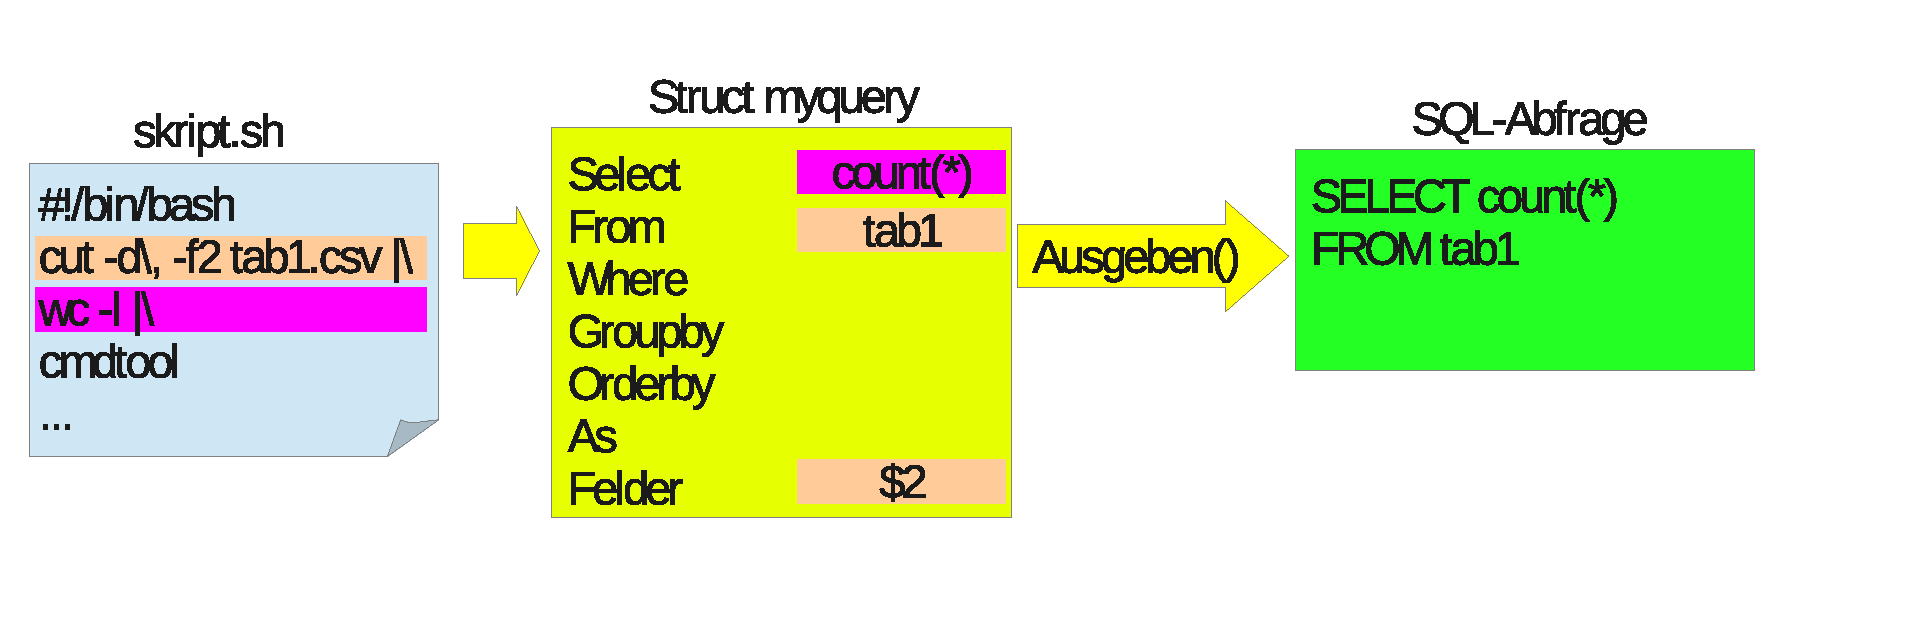
\includegraphics[scale=.35]{parser1.eps}
\caption{Arbeitsweise des Yacc Bash2SQL-Parsers}
\label{fig:parser1}
\end{figure}

Die Idee ist jetzt, für jedes Kommando eine Regel zu erstellen, die in Abhängigkeit des Kommandos (für jedes Kommando ein Token) die Abfrage anders modifiziert. Eine Regel der Grammatik besteht immer zuerst aus dem Kommando und dann weiteren Parametern:

\begin{lstlisting}[language=Bash]
<Kommando> [Optionen] Datei [Optionen]
\end{lstlisting}

Die Aktionen werden entsprechend ausgeführt:
\begin{itemize}
\item \textbf{cat [dateiname]}: der Dateiname ist die gewünschte CSV-Datei und entspricht dem Tabellennamen, also kann der Name so in die From-Klausel übernommen werden
\item \textbf{cut Optionen [dateiname]}: wieder ist der Dateiname (sofern angegeben) die gewünschte Tabelle, die Optionen werden mit einer eigenen Regel extra geparst
\item \textbf{grep Muster [Dateiname]}: wieder analog, nur dass ein Muster angegeben ist, also ein Prädikat. Die Funktion \lstinline{zugrep()} erzeugt eine Bedingung die in jeder Spalte nach Vorkommen des Musters sucht
\end{itemize}

\subsection{Bedienung des Bash2SQL-Übersetzers}
Im Ordner \textit{bash\_parser\_yacc} liegen die Dateien \textit{bash2sql.lex} und \textit{bash2sql.y}, also die Lexer-Regeln und die Yacc-Grammatik. Das beiliegende Makefile kompiliert aus den Dateien das Programm \textit{kleinerParser} (s. Abb. \ref{fig:lexyacc}), das aus einfachen Shell-Skripten SQL-Abfragen erzeugt.

\begin{figure}[h]
\centering
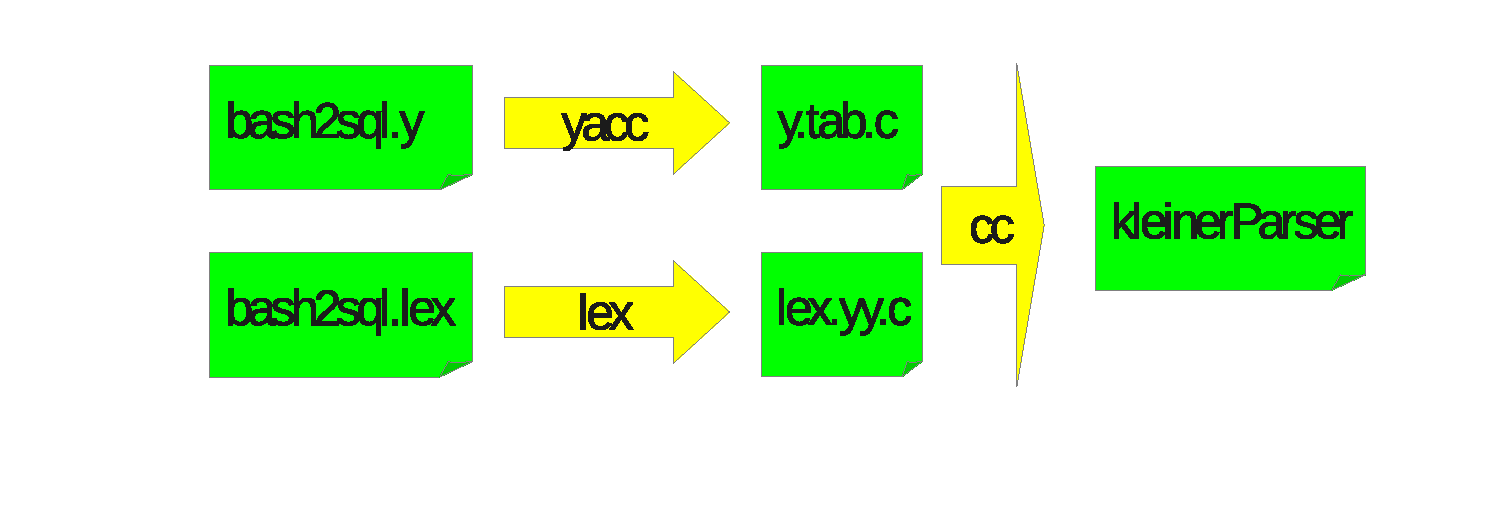
\includegraphics[scale=.3]{yacc.eps}
\caption{Zusammenspiel von Lex und Yacc}
\label{fig:lexyacc}
\end{figure}

Der Übersetzer arbeitet als einfacher Filter, er liest von der Standardeingabe und gibt auf der Standardausgabe das Ergebnis aus. Ein Befehl kann direkt übersetzt werden.

\begin{lstlisting}[language=Bash]
$ echo "cat tabelle | cut -f1,2,3 | grep Muster" | ./kleinerParser
\end{lstlisting}

Oder ein Befehl wird aus einer Datei gelesen.
\begin{lstlisting}[language=Bash]
$ cat abfrage.sh | ./kleinerParser
\end{lstlisting}

In beiden Fällen wird folgende Ausgabe erzeugt:
\begin{lstlisting}[language=SQL]
SELECT $1,$2,$3, FROM tabelle WHERE ($1 like '%Muster%'
	or $2 like '%Muster%' or $3 like '%Muster%' 
	or false) GROUP BY  ORDER BY  AS
\end{lstlisting}

Da die Spaltennamen noch nicht eingelesen werden, werden sie manuell ersetzt. Bis auf ein paar Schönheitsfehler ist die Abfrage in Ordnung.

\chapter{Parser mit ANTLR}
Der bisherige Parser unterstüzt nur sehr wenige Befehle, implementiert noch die gesamte Shell-Grammatik und bedarf einiger Korrekturen um korrekte SQL-Syntax zu erzeugen. Dabei lohnt sich gleich der Umstieg auf \textbf{ANTLR}, einen mächtigeren Parser-Generator, der außerdem den Code in verschiedenen Programmiersprachen erzeugen kann.
\section{Konfiguration}
Der ANTLR-Parser basiert auf Java und erzeugt ohne Erweiterung nur Parser in dieser Sprache, für andere Zielsprachen ist eine Bibliothek zu installieren.

\subsection{Installieren der Bibliothek}
Für einen Parser in C/C++ wird die Bibliothek \textit{libantlr3c-3.4}
\footnote{\label{foot:1}erhätlich unter \url{http://www.antlr3.org/download/}}
benötigt, sie enthält alle benötigten Funktionen bzw. Klassen.
Die Datei herunterladen, entpacken, konfigurieren und installieren. Dabei ist folgendermaßen vorzugehen:
\begin{lstlisting}[language=Bash]
tar -xzf libantlr3c-3.4.tar.gz
cd libantlr3c-3.4
./configure --enable-64bit
make
make install
\end{lstlisting}
Läuft das Programm auf einem 32-Bit-System, so ist der dritte Schritt durch \textit{./configure} zu ersetzen. Anschließend ist die Bibliothek in \textit{/usr/local/lib} installiert.

\subsection{Starten von ANTLR}
Zuerst muss der Parsergenerator als \textit{antlr-3.5.2-complete.jar} \ref{foot:1} heruntergeladen werden, aber in der Version 3.5.2, da neuere Versionen noch nicht die Codegenerierung in andere Sprachen beherrschen.
Für den folgenden Schritt wird angenommen, dass die jar-Datei in \textit{\~{}/Downloads} liegt.
Bevor der Parser-Code generiert werden kann, muss der Klassenpfad für Java und der Pfad zur Bibliothek gesetzt werden, damit die Java Virtual Machine die Komponenten von ANTLR findet und die Bibliothek eingebunden ist.
\begin{lstlisting}[language=Bash]
export LD_LIBRARY_PATH=/usr/local/lib:$LD_LIBRARY_PATH
export CLASSPATH=~/Downloads/antlr-3.5.2-complete.jar:$CLASSPATH
\end{lstlisting}

\subsection{Vorwissen zu ANTLR}
Im Gegensatz zu anderen Parsern ist ANTLR in einer objektorientierten Sprache geschrieben (wie schon erwähnt in Java), so realisiert er Lexer und Parser als zwei verschiedene Klassen. ANTLR ist mächtiger als Yacc mit Lex, da die lexikalische Analyse auch kontextsensitive Grammatiken unterstützt, LEX nur kontextfreie.
Außerdem ist es in ANTLR möglich, die Regeln für die lexikalische und grammatikalische Analyse in eine Grammatik-Datei zu packen, können aber - dank Modularität - auf mehrere aufgeteilt werden. Die Dateien enden auf \textit{.g} und folgen dem Schema:\cite{antlr}
\begin{lstlisting}
<Grammatik-Typ> grammar <name>;
<Optionen>
<Token-Definition>
<Quellcode>
<Grammatik-/Lexer-Regeln>
\end{lstlisting}

In den Bereich für den Quellcode können sowohl die Kopfzeilen und Deklarationen, wie auch die Funktionen angegeben werden, der Teil kombiniert also den zweiten und letzten Bereich des Schemas von Yacc, dennoch sind sie mit einem Schlüsselwort voneinander abzugrenzen:
\begin{lstlisting}
@header
{
/* Parser-Kopf */
}
@members
{
/*  Parser-Rumpf */
}
\end{lstlisting}

Die Lexer-Definitionen erfolgen analog durch die Schlüsselworte \textit{@lexer::header} und \textit{@lexer::members}. Die anderen Teile stehen für Folgendes:
\begin{enumerate}
\item <Grammatik-Typ> entweder Lexer, Parser oder AST, fehlt die Angabe, so Lexer und Parser kombiniert
\item <Optionen> unter anderem die Zielsprache
\item <Token-Definition> und <Quellcode> sind analog zu Yacc und Lex
\item <Grammatik-/Lexer-Regeln> sind die gewünschten Regeln
\end{enumerate}
Ein schönes und einfaches Beispiel findet sich auf der Homepage \url{www.antlr.org}, im Nachfolgenden werden nur die Zielsprachen C/C++ betrachtet.
\newpage
\section{Der Bash2SQL-Übersetzer mit ANTLR in C}
Dieses Mal soll die komplette Bash-Grammatik geparst werden können, die Abfragen sollen modularer und syntaktisch korrekt aufgebaut sein und mittels ANTLR für C generiert.

\subsection{Neues Konzept}
Bisher sind die Kommandos der Reihe nach geparst und in eine SQL-Abfrage übersetzt worden, bis es nicht mehr geht, wenn ein Kommando unbekannt ist. Jetzt ist die Überlegung, dass jedes Kommando für sich allein steht und eine eigene SQL-Abfrage ergibt. Die Ausgabe erfolgt über den Standardfluss, kann also mit weiteren Kommandos durch eine Pipe verbunden werden (s.\ Abb. \ref{fig:parser2}).

\begin{figure}[h]
\centering
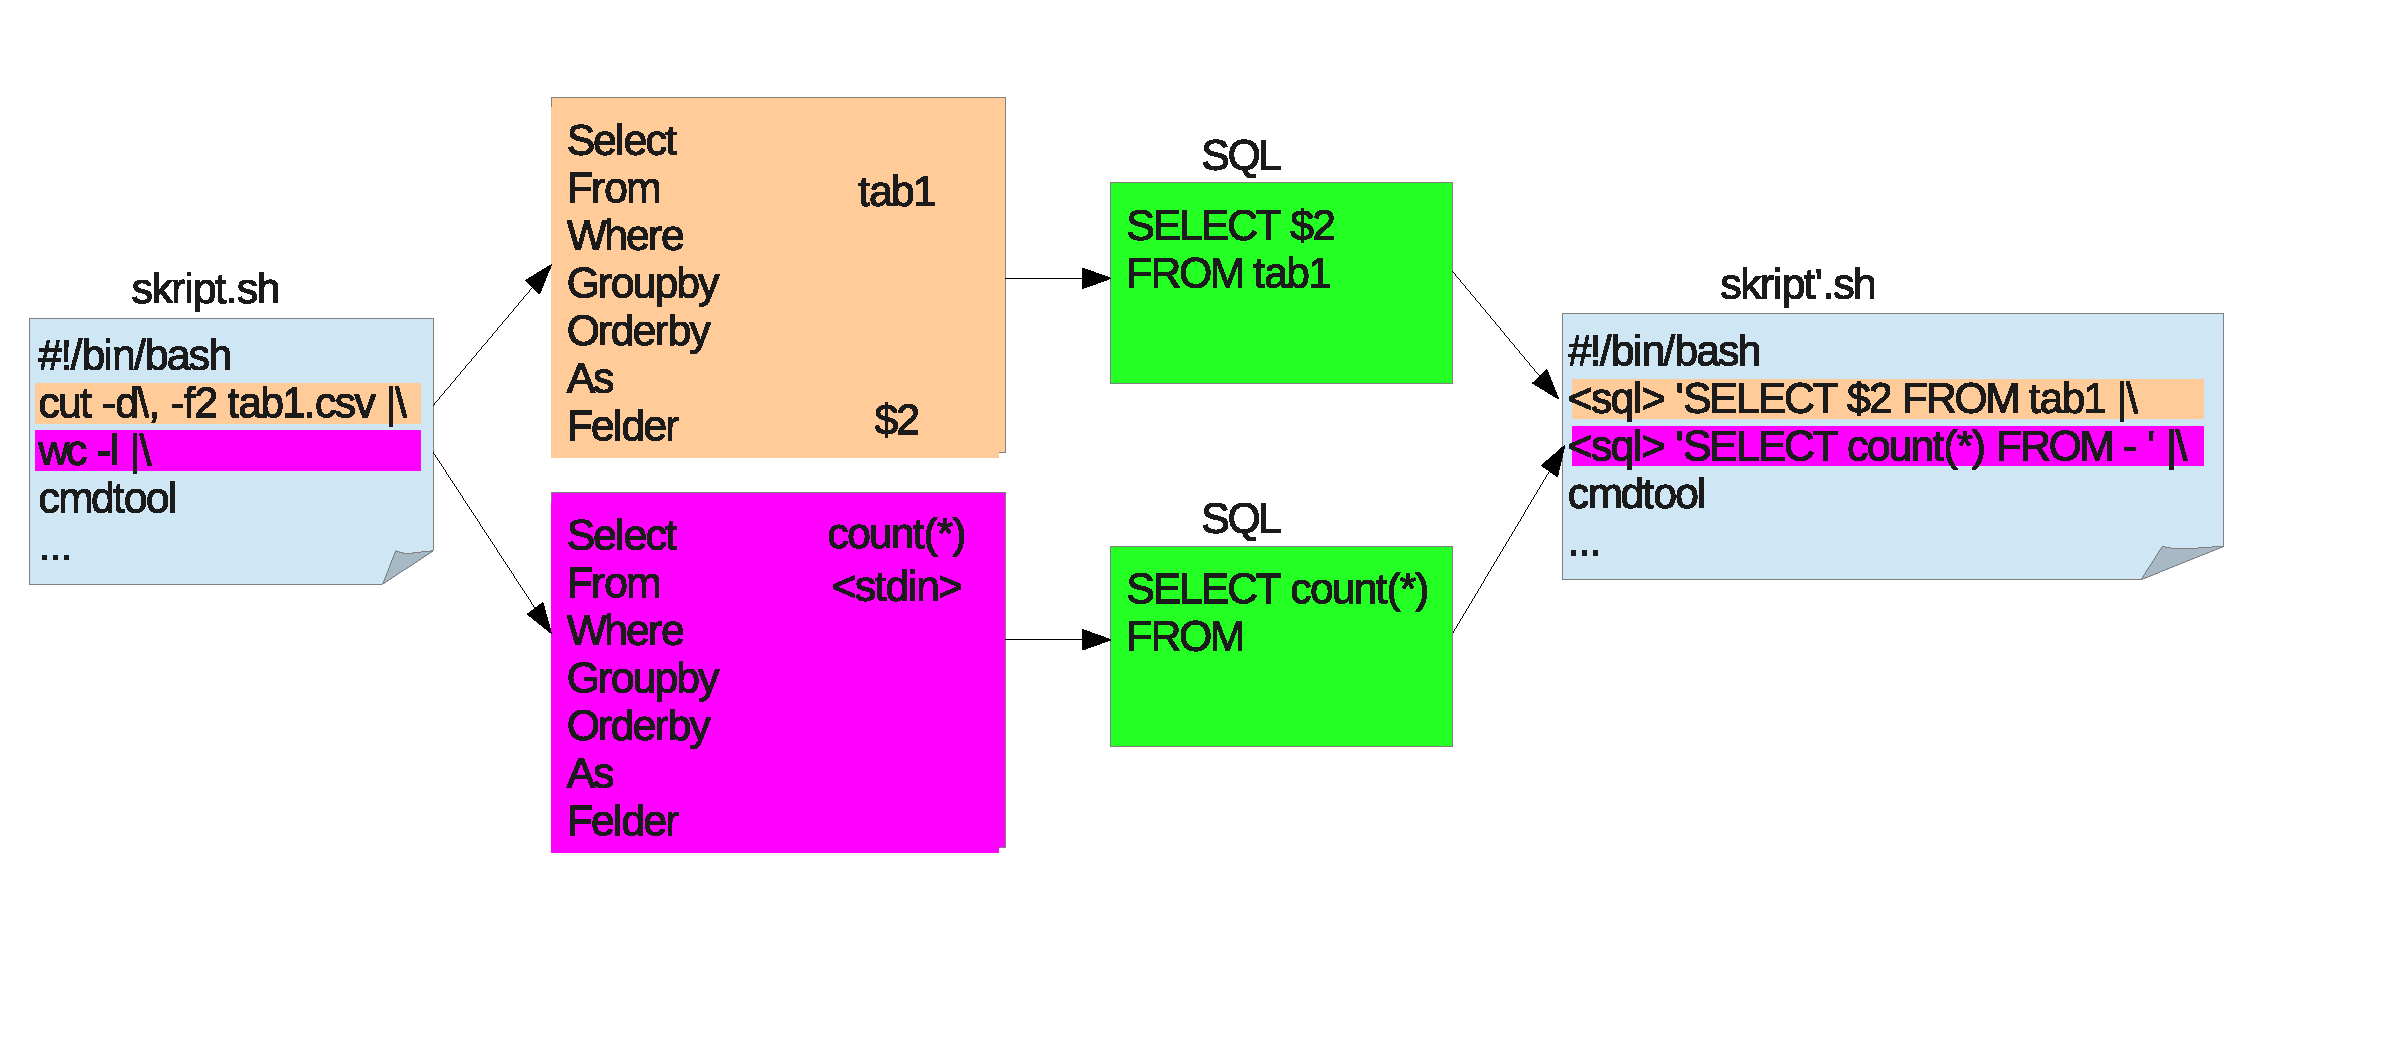
\includegraphics[scale=.4]{parser2.eps}
\caption{Neues Konzept}
\label{fig:parser2}
\end{figure}

Schöner ist es natürlich, wenn der Übersetzer gleich erkennt, wann er welche Abfragen zusammenfügen kann, sodass am Ende eine geschachtelte SQL-Abfrage entsteht, die auch optimiert werden kann. Das ist besser, als wenn jede Abfrage einzeln ausgewertet wird und die Kommunikation mit Hilfe der Shell erfolgt, die die Daten über den Strom schickt. Die vorgestellte Idee wird modifiziert, indem der Parser solange die Kommandos liest, bis er am Ende ist oder ein ihm unbekanntes Kommando erscheint. Für jedes gelesene Kommando wird eine Abfrage erstellt, die die vorherige, falls existent, als Quelltabelle aufnimmt. Daraufhin entsteht eine geschachtelte SQL-Anweisung. Im Moment steht diese dann zwischen allen nicht erkannten Kommandos, sodass ein wieder funktionierendes Skript erzeugt wird (s. Abb. \ref{fig:parser3}).

\begin{figure}[h]
\centering
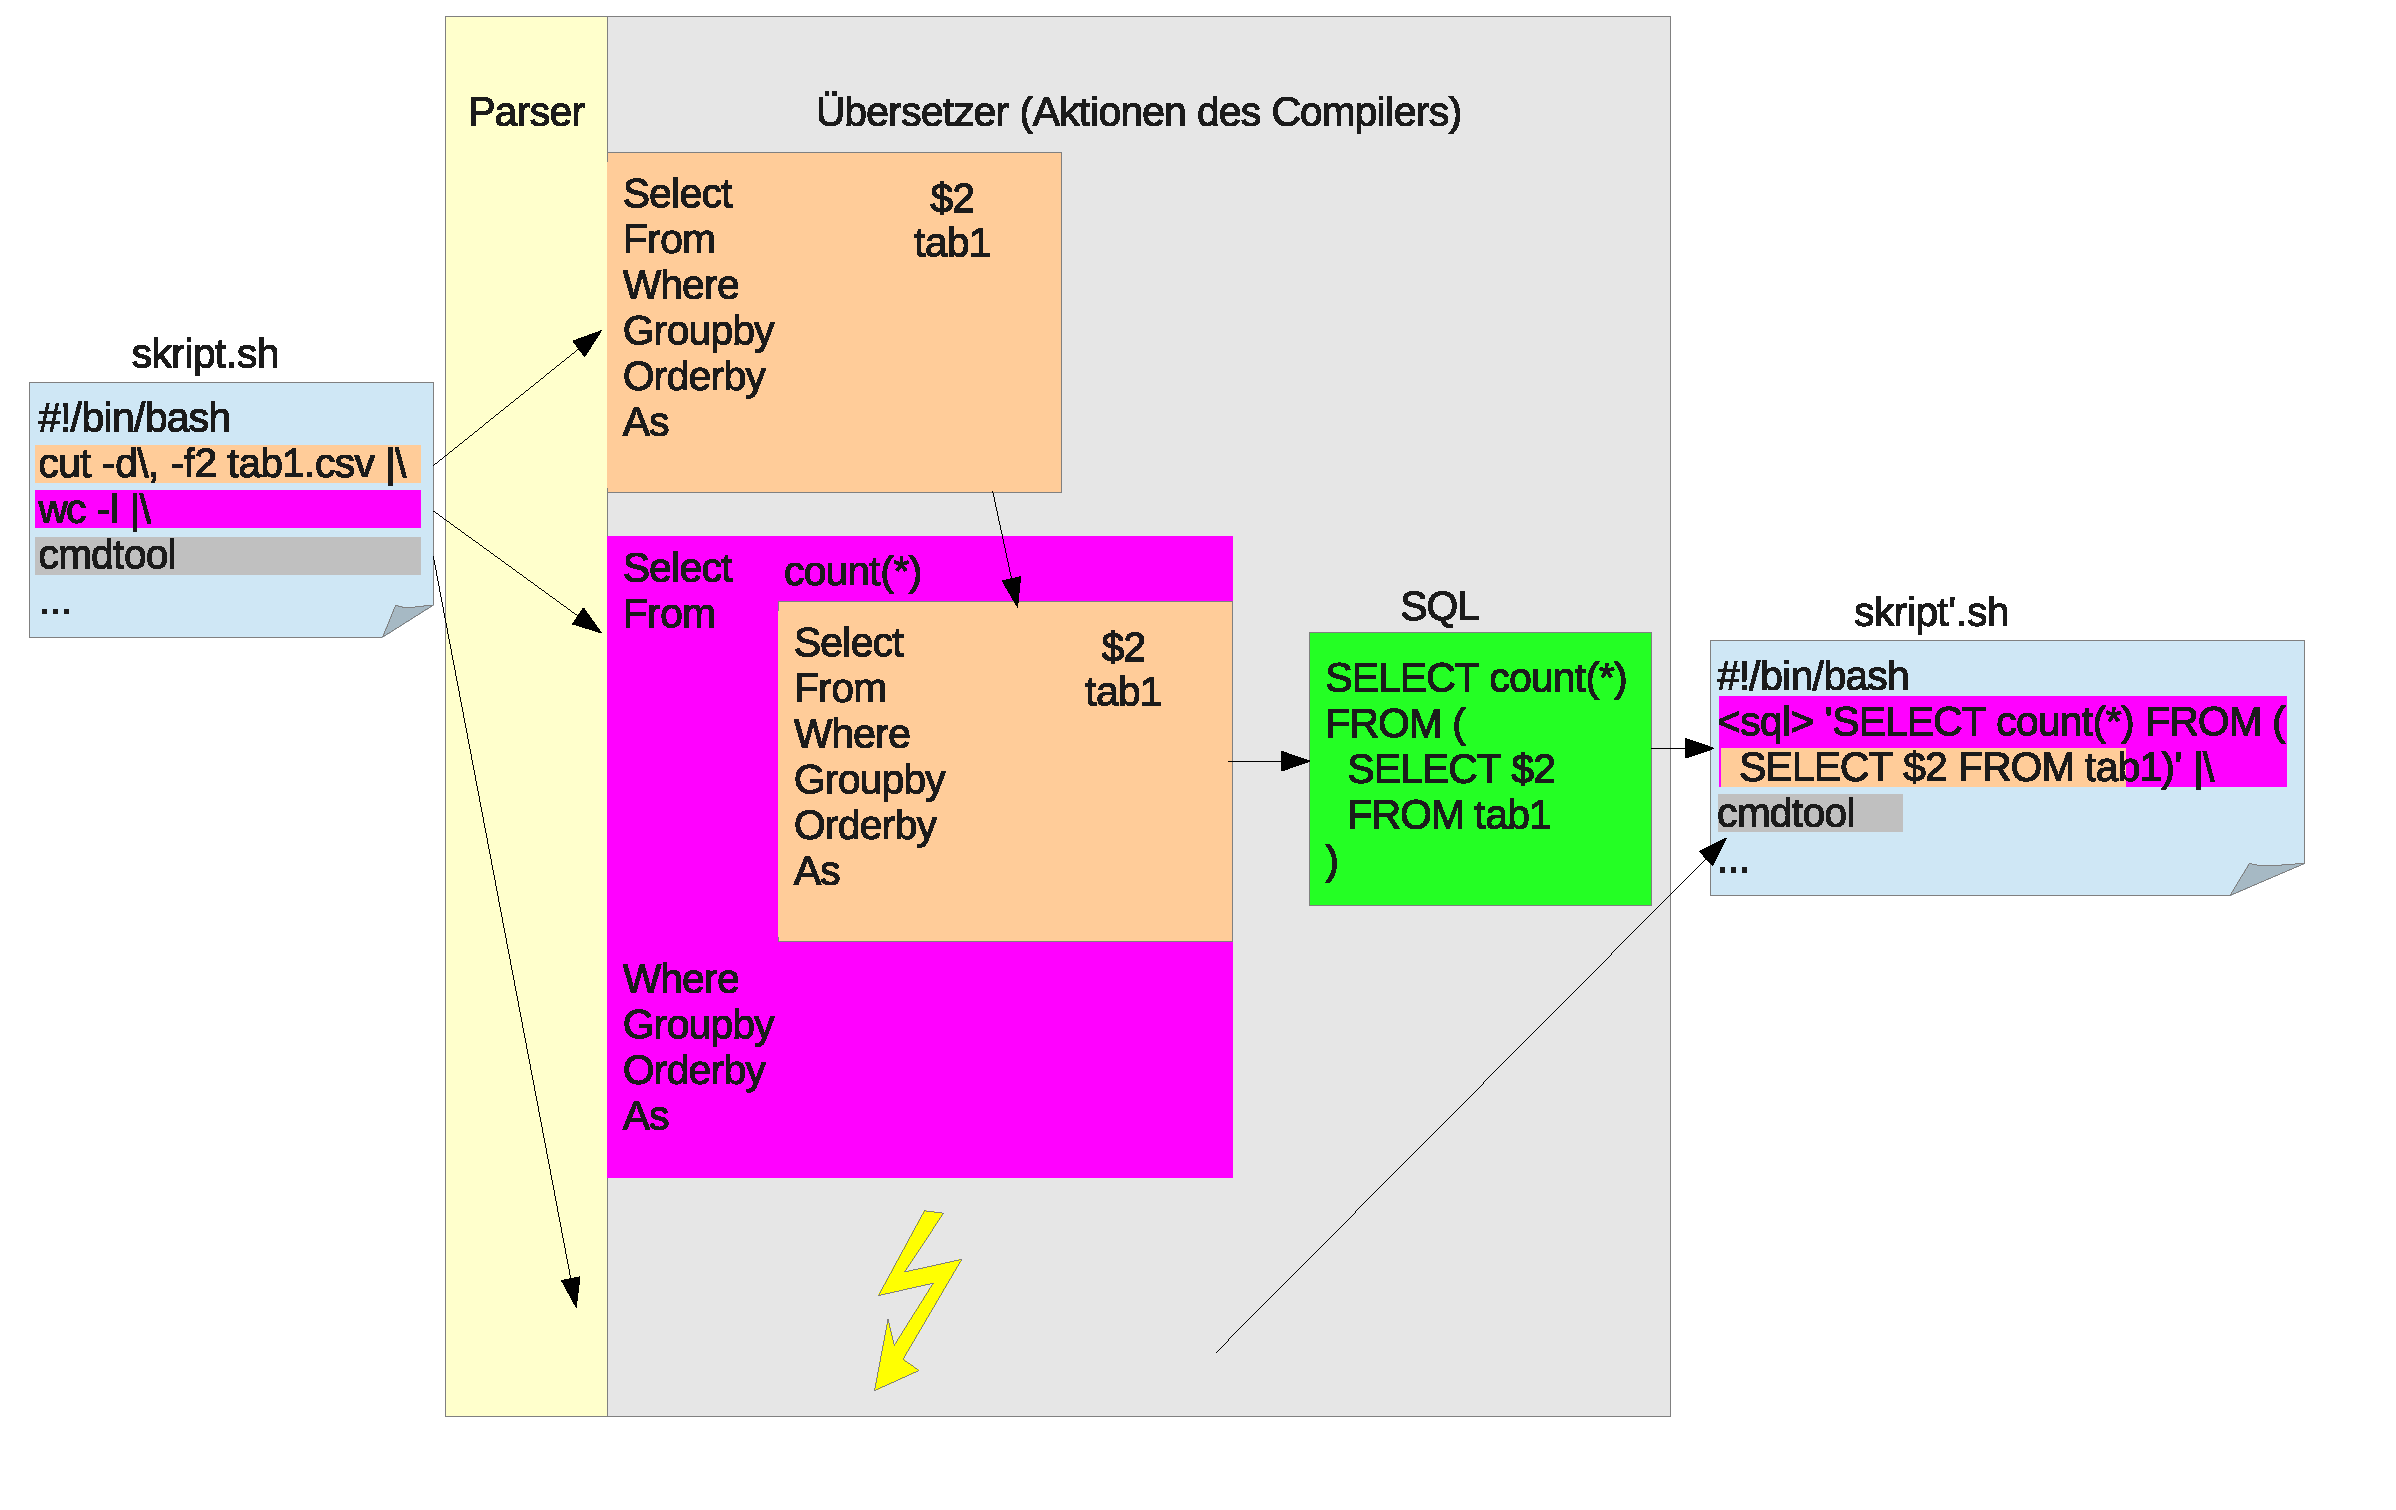
\includegraphics[scale=.4]{parser3.eps}
\caption{Neues Konzept mit Schachtelung}
\label{fig:parser3}
\end{figure}

\subsection{C-Quellcode}
Die Definition des SQL-Abfrage-Structs, um die Abfrage aufzunehmen, ist bis auf einige Erweiterungen um Joins und Vereinigungen zu bilden identisch zu der des Parsers in Yacc.
Zuerst muss natürlich die Shell-Grammatik implementiert sein, praktischerweise existieren zahlreiche Bücher, die die Grammatik in Backus-Naur-Form beschrieben haben und sich somit leicht in ANTLR importieren lässt \cite{Shell-BNF}.

\subsection{Die Grammatik}
Besonders interessant ist die Stelle, die für die Ausgabe der SQL-Anweisung zuständig ist, die Regel \textit{pipeline\_cmd}. Sie erkennt die Konkatenation mehrerer Befehle (\textit{command}) mittels einer Pipe. Die Kommunikation erfolgt über eine Referenz auf den letzten SQL-Abfrage-Struct \textit{lastquery}, ist dieser \textit{NULL}, so konnte das Kommando nicht geparst werden und der Befehl soll wieder ausgegeben werden. Alternativ wird am Ende der SQL-Abfrage-Struct ausgegeben. Das Attribut \textit{tobeprint} dient zum Erkennen, ob zuerst der Kopf einer Schleife ausgegeben werden soll.

\begin{lstlisting}
pipeline_cmd    : c1=command
                        {
                        if(tobeprint && !lastquery && $c1.text->chars)
                                printf("\%s",$c1.text->chars);
                        }
                (PIPE c2=command
                        {
                        if(tobeprint && !lastquery)
                                printf(" | \%s",$c2.text->chars);
                        }
                )*
                {
                if(lastquery)
                        ausgeben(lastquery);
                printf("\n");
                tobeprint=1;
                }
        ;
\end{lstlisting}

Auf diese Weise steigt man ab bis zur Regel \textit{cmd}, in der die Übersetzung der Kommandos implementiert ist.
\begin{lstlisting}
cmd returns [query *r]
\end{lstlisting}

Als Parameter können Optionen oder die anzuzeigende Datei angegeben werden. Optionen (das Lexer-Token \textit{OPTS}) werden mit der Methode \textit{optscut()} gleich analysiert und das Ergebnis in den Struct eingebunden. Für jedes Kommando existiert eine eigene Funktion, um die Optionen zu parsen, also die eine Zeichenkette nimmt und sie Buchstabe für Buchstabe abarbeitet.\\

Mit den vorgestellten Methoden und Regeln ist es nun möglich, komplette Bash-Skripte zu parsen und die unterstützten Kommandos zu interpretieren.

\subsection{Bedienung}
Im Ordner \textit{c\_bash\_parser\_antlr} liegen die Grammatikdatei \textit{SimpleBashSQL.g} und ein Makefile. Beide reichen aus, um mit \textit{make} den Parser zu erzeugen, wenn die Bibliothek richtig installiert und die Pfade richtig gesetzt sind.\\
ANTLR erzeugt eine Lexer- und eine Parser-Quelldatei \textit{SimpleBashSQL\{Lexer,Parser\}.\{h,c\}}, die zu dem fertigen Compiler mittels \textit{cc} kompiliert werden:

\begin{lstlisting}[language=make]
all: simplebashsql

simplebashsql: $(OBJ).g
        java org.antlr.Tool $^
        gcc -g -o $@ -I/usr/local/include/ -L/usr/local/lib/ -lantlr3c $(OBJ)Parser.c $(OBJ)Lexer.c
\end{lstlisting}

Das Programm nimmt den Dateinamen eines Skripts als Eingabeparameter und schickt das Ergebnis auf die Standardausgabe. So wird das Skript:
\begin{lstlisting}[language=Bash]
#!/bin/bash
cut -f1,2,3 vorlesungen.csv | sort -k2
\end{lstlisting}
übersetzt in:
\begin{lstlisting}
#!/bin/bash
SELECT VorlNr,Titel,SWS FROM  (
	SELECT VorlNr,Titel,SWS FROM vorlesungen.csv AS b
) AS b ORDER BY $1 
\end{lstlisting}
\newpage
\section{Der Bash2SQL-Übersetzer mit ANTLR in C++}
So schön die Sprache C auch ist, so ist die Speicherverwaltung mit ihr ziemlich anstrengend, vor allem da die Bezeichner von Tabellen oder Spalten unterschiedlich lang werden, lohnt sich der Umstieg auf C++ mit impliziter Speicherverwaltung und einer Standardbibliothek mit \textit{vector} und \textit{string}, die einem das Leben erleichtern. Außerdem kann ein höheres Abstraktionsniveau erreicht werden, indem die Abfrage über eine eigene Klasse gekapselt wird und der Zugriff nur noch über Methoden erfolgt.

\subsection{Unterschiede: C vs. C++ mit ANTLR}
Um ANTLR C++-Code generieren zu lassen, sind einige Änderungen nötig.
Die Unterstützung von C++ in ANTLR baut auf sogenannten Traits auf, also vorgefertigten Klassen die in ähnlicher Weise wiederverwendet werden, in dem vorliegenden Fall für den Lexer.

\begin{lstlisting}[language=C++]
@lexer::traits {
     class  SimpleBashSQLLexer;
     class  SimpleBashSQLParser;
     typedef antlr3::Traits< SimpleBashSQLLexer, SimpleBashSQLParser > SimpleBashSQLLexerTraits;
     typedef SimpleBashSQLLexerTraits SimpleBashSQLParserTraits;
}
\end{lstlisting}

Die Header-Dateien, in denen die verwendeten Klassen wie \textit{antlr3} definiert sind, müssen zum Kompilieren eingebunden werden. Die Dateien finden sich im \textit{antlr3-master} (erhätlich bei github
\footnote{\url{https://github.com/antlr/antlr3}})
im Verzeichnis \textit{antlr3-master/runtime/Cpp/include}.

Die Main-Methode muss natürlich noch verändert werden, die Funktionsweise ist aber identisch zum Parser in C, die einzulesende Datei wird als Operand mitgegeben.

\begin{lstlisting}[language=C++]
int main(int argc, char * argv[])
{
	if(argc!=2){
		printf("\%s: fehlender Operand\n",argv[0]);
		return 1;
	}

	ANTLR_UINT8* fName = (ANTLR_UINT8*) argv[1];
	SimpleBashSQLLexer::InputStreamType input(fName, ANTLR_ENC_8BIT);
	SimpleBashSQLLexer lxr(&input); // TLexerNew is generated by ANTLR
	SimpleBashSQLParser::TokenStreamType tstream(ANTLR_SIZE_HINT, lxr.get_tokSource() );
	SimpleBashSQLParser psr(&tstream); // TParserNew is generated by ANTLR3
	psr.file();
	return 0;
}
\end{lstlisting}

Um in den Aktionen auf den Wert eines Symbols zugreifen zu können, dienen Ströme (Streams). Soll der Wert ausgegeben werden, so erfolgt der Zugriff über das Attribut \textit{text}, zum Beispiel eine Ausgabe auf der Standardausgabe:
\begin{lstlisting}[language=C++]
comment { std::cout << $comment.text; }
\end{lstlisting}

\subsection{Die Klasse TheQuery}
Für die erste fundamentale Änderung werden alle Operationen für eine Abfrage in der Klasse \textit{TheQuery} gekapselt. Alle Veränderungen am Datenbestand erfolgen jetzt über Methoden, die interne Repräsentation interessiert den späteren Compiler nicht und das Praktische daran: die Klasse steht für sich allein und ist auch komplett austauschbar durch ein Substitut, das nur die entsprechenden Schnittstellen implementieren muss.
Der Aufbau der Klassen orientiert sich an der DB2-Referenz von IBM, die schön modular beschrieben ist \cite{db2}.

\subsubsection{Interne Repräsentation}
\begin{figure}[h]
\centering
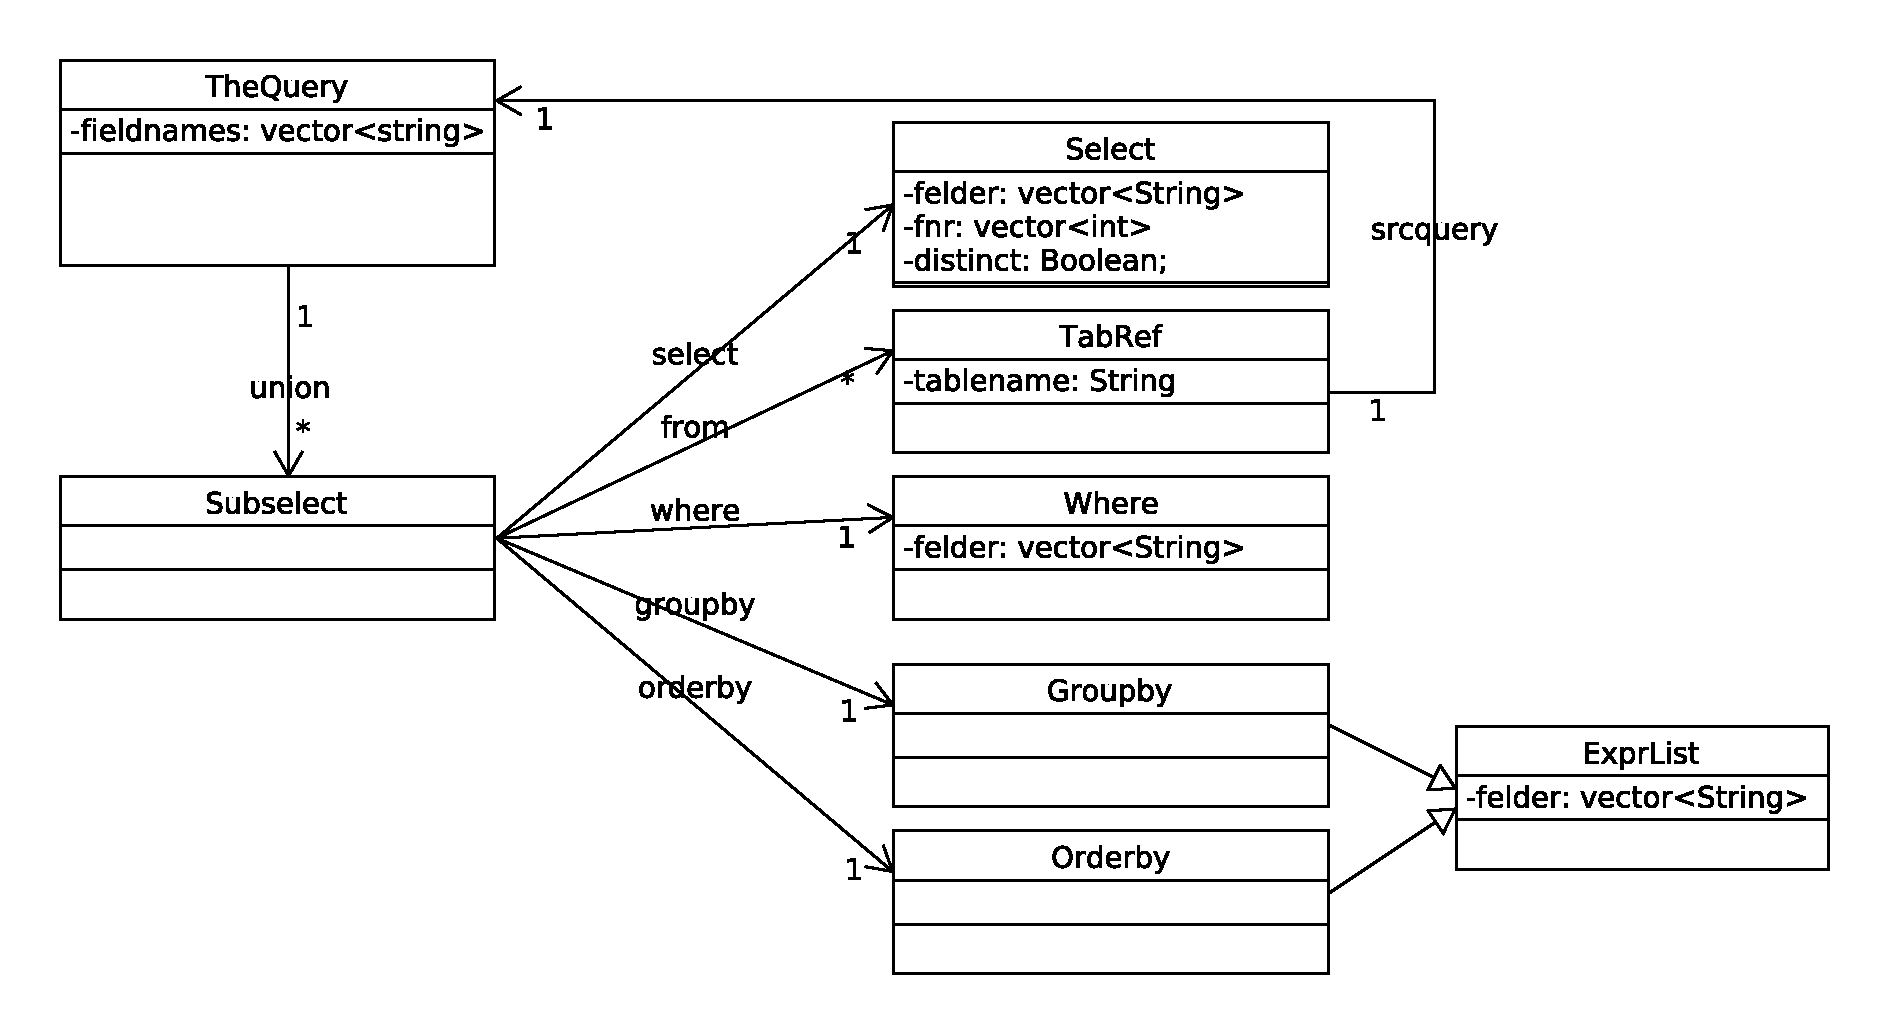
\includegraphics[scale=.4]{TheQuery.eps}
\caption{Aufbau der Klasse TheQuery}
\label{fig:TheQuery}
\end{figure}
Eine Klasse besteht aus einer Hauptklasse \textit{TheQuery}, die auch alle Methoden für den Zugriff kapselt (s. Abb. \ref{fig:TheQuery}). Sie verantwortet die Mengen aus mehreren eigentlichen Abfragen durch Vereinigung (vector<Subselect> union) oder durch die im Moment nicht benötigte Schnittmenge oder Differenz.
Die Klasse \textit{Subselect} bildet die eigentliche Abfrage mit einer \textit{Select}-Clause, einer Menge \textit{vector<TabRef> from} als Referenztabelle und den Objekten für Prädikate (\textit{Where}), Gruppierungen (\textit{Groupby}) und Sortierungen (\textit{Sortby}). Letztere beiden sind ähnlich als Vektor aus Feldern implementiert und erben noch von einer solchen Klasse \textit{ExprList}. Die Prädikate der Where-Klausel sind durch Konjunktionen (\textit{AND}) verknüpfte Aussagen und im Nachfolgenden wird eine konjunktive Normalform eingehalten, sodass eine Konjunktion aus Disjunktionen erstellt ist. In manchen Fällen wird als neutrales Element \textit{true} verwendet, wenn eine Aussage entfernt wird. Für Tabellen dient eine Klasse \textit{TabRef} mit einem Tabellennamen oder einer Referenz auf eine komplette Abfrage als Quelle. Die Referenz ist geeigneter als eine Vererbung, da die Klasse auch die textuelle Ausgabe mit einer entsprechenden Klammerung steuert.

\subsubsection{Darstellung der Felder}
Eine Schwierigkeit stellt die interne Repräsentation der Felder dar, da die Spaltenbezeichner nicht aus den Skripten hervorgehen und nicht davon auszugehen ist, dass die Bezeichner aus einer Datei auszulesen sind. Deshalb werden vorübergehend die Feldbezeichner entsprechend zu awk gewählt (\textit{\$1,\$2,...}), das Maximum an Spalten muss dann definiert werden, wie gewohnt in \textit{MAXFIELDS}. Die gewählten Felder können direkt in die Select-Klausel eingefügt werden, auch als Zahlenvektor.

\begin{lstlisting}[language=C++]
void Select::addSelect(std::vector<int> feldnr)
{
        fnr=feldnr;
        /*copies values into felder*/
        for (std::vector<int>::iterator it = fnr.begin();
                it!=fnr.end(); it++){
                std::stringstream stmp;
                stmp << "$" << *it;
                felder.push_back(stmp.str());
        }
}
\end{lstlisting}

Jedes Mal, wenn ein Tabellenname in die Abfrage eingelesen wird, wird überprüft, ob eine passende Datei mit passender Kopfzeile vorhanden ist. Die Spalten werden mit der Methode \lstinline{getnamesfromfile()} eingelesen, das Spaltentrennzeichen \textit{DELIMIT} wird durch eine Präprozessoranweisung definiert.

\begin{lstlisting}[language=C++]
/*union more queries*/
void TheQuery::makeUnion(string src)
{
        /* table already defined? */
        if(queries[0]->notable())
                queries[0]->addTable(src);
        else
                queries.push_back(new Subselect(src));

        /*add column names*/
        getnamesfromfile(src,DELIMIT);
}
\end{lstlisting}

Die Methode \lstinline{getnamesfromfile()} setzt die Spaltennamen in \textit{fieldnames}, wenn noch nicht definiert, mit der Methode \lstinline{lookup()}. Diese Methode liest die erste Spalte einer Datei, trennt die Zeile nach dem Trennzeichen und gibt einen Vektor der Klasse String zurück.
\begin{lstlisting}[language=C++]
std::vector<std::string> TheQuery::lookup(std::string filename, char delimit)
{
        FILE *f;
        char * line = NULL;
        size_t len = 0;
        ssize_t read;
        char** ptr;
        std::vector<std::string> tmp;
        f=fopen(filename.c_str(),"r");
        if(!f)
                return std::vector<std::string>();
        if( read = getline(&line, &len, f) ==-1)
                return std::vector<std::string>();
        fclose(f);

        tmp=str_split(line,delimit);
        /* header columns terminated with delimiter symbol */
        tmp.pop_back();
        return tmp;
}
\end{lstlisting}

Das Attribut \textit{fieldnames} ist für das ganze Objekt einer Klasse \textit{TheQuery} gültig, da bei jeder Teilabfrage einer Vereinigung auch die Spaltenbezeichner identisch sein müssen. Bei Bildung eines Kreuzproduktes werden die hinzukommenden Spalten einfach hinzugefügt. Wird die Abfrage in einer anderen verwendet, so werden auch die Spaltennamen übergeben.

\begin{lstlisting}[language=C++]
void TheQuery::makeUnion(TheQuery* src)
{
        if(src==NULL)
                return;
        /* table already defined? */
        if(queries[0]->notable())
                queries[0]->addTable(src);
        else
                queries.push_back(new Subselect(src));
        /*get columnnames from file*/
        if(fieldnames.size()==0)
                fieldnames=src->getColumns();
}
\end{lstlisting}

Bevor eine Abfrage mit \textit{print()} ausgegeben wird, werden alle Hilfsspaltenbezeichner, die durch Dollar gekennzeichnet sind, ersetzt. Dazu stellt mit \lstinline{replace_dollars()} jede Klasse eine Methode zur Verfügung, die intern die Hilfsbezeichner ersetzt durch den passenden Spaltennamen aus \textit{fieldnames}.

\begin{lstlisting}[language=C++]
void TheQuery::print()
{
        /*only when a query is defined, should always be the case*/
        if(queries.size()>0){
                queries[0]->replace_dollars(fieldnames);
                queries[0]->print();
        }
        /* union all queries */
        for(int i=1; i<queries.size(); i++){
                std::cout << " UNION ";
                queries[i]->replace_dollars(fieldnames);
                /*now all unions must have an unique id*/
                queries[i]->print(i);
        }
}
\end{lstlisting}

Soweit steht die Klasse TheQuery und kann zur Erstellung der Abfragen genutzt werden, der Zugriff erfolgt nur über die Methoden von TheQuery.

\subsection{Der Parser näher betrachtet}
Der Übersetzer bzw. Compiler besteht aus zwei Teilen, zuerst wird der Syntax analysiert und ein Syntaxbaum generiert, dann können die zugehörigen Aktionen ausgeführt werden (vgl. Abbildung \ref{fig:parsen}). Dabei hat sich wenig verändert, die Syntaxanalyse funktionert in C++ etwas flexibler, manche Lexerregeln können besser gestaltet werden.

\begin{figure}[h]
\centering
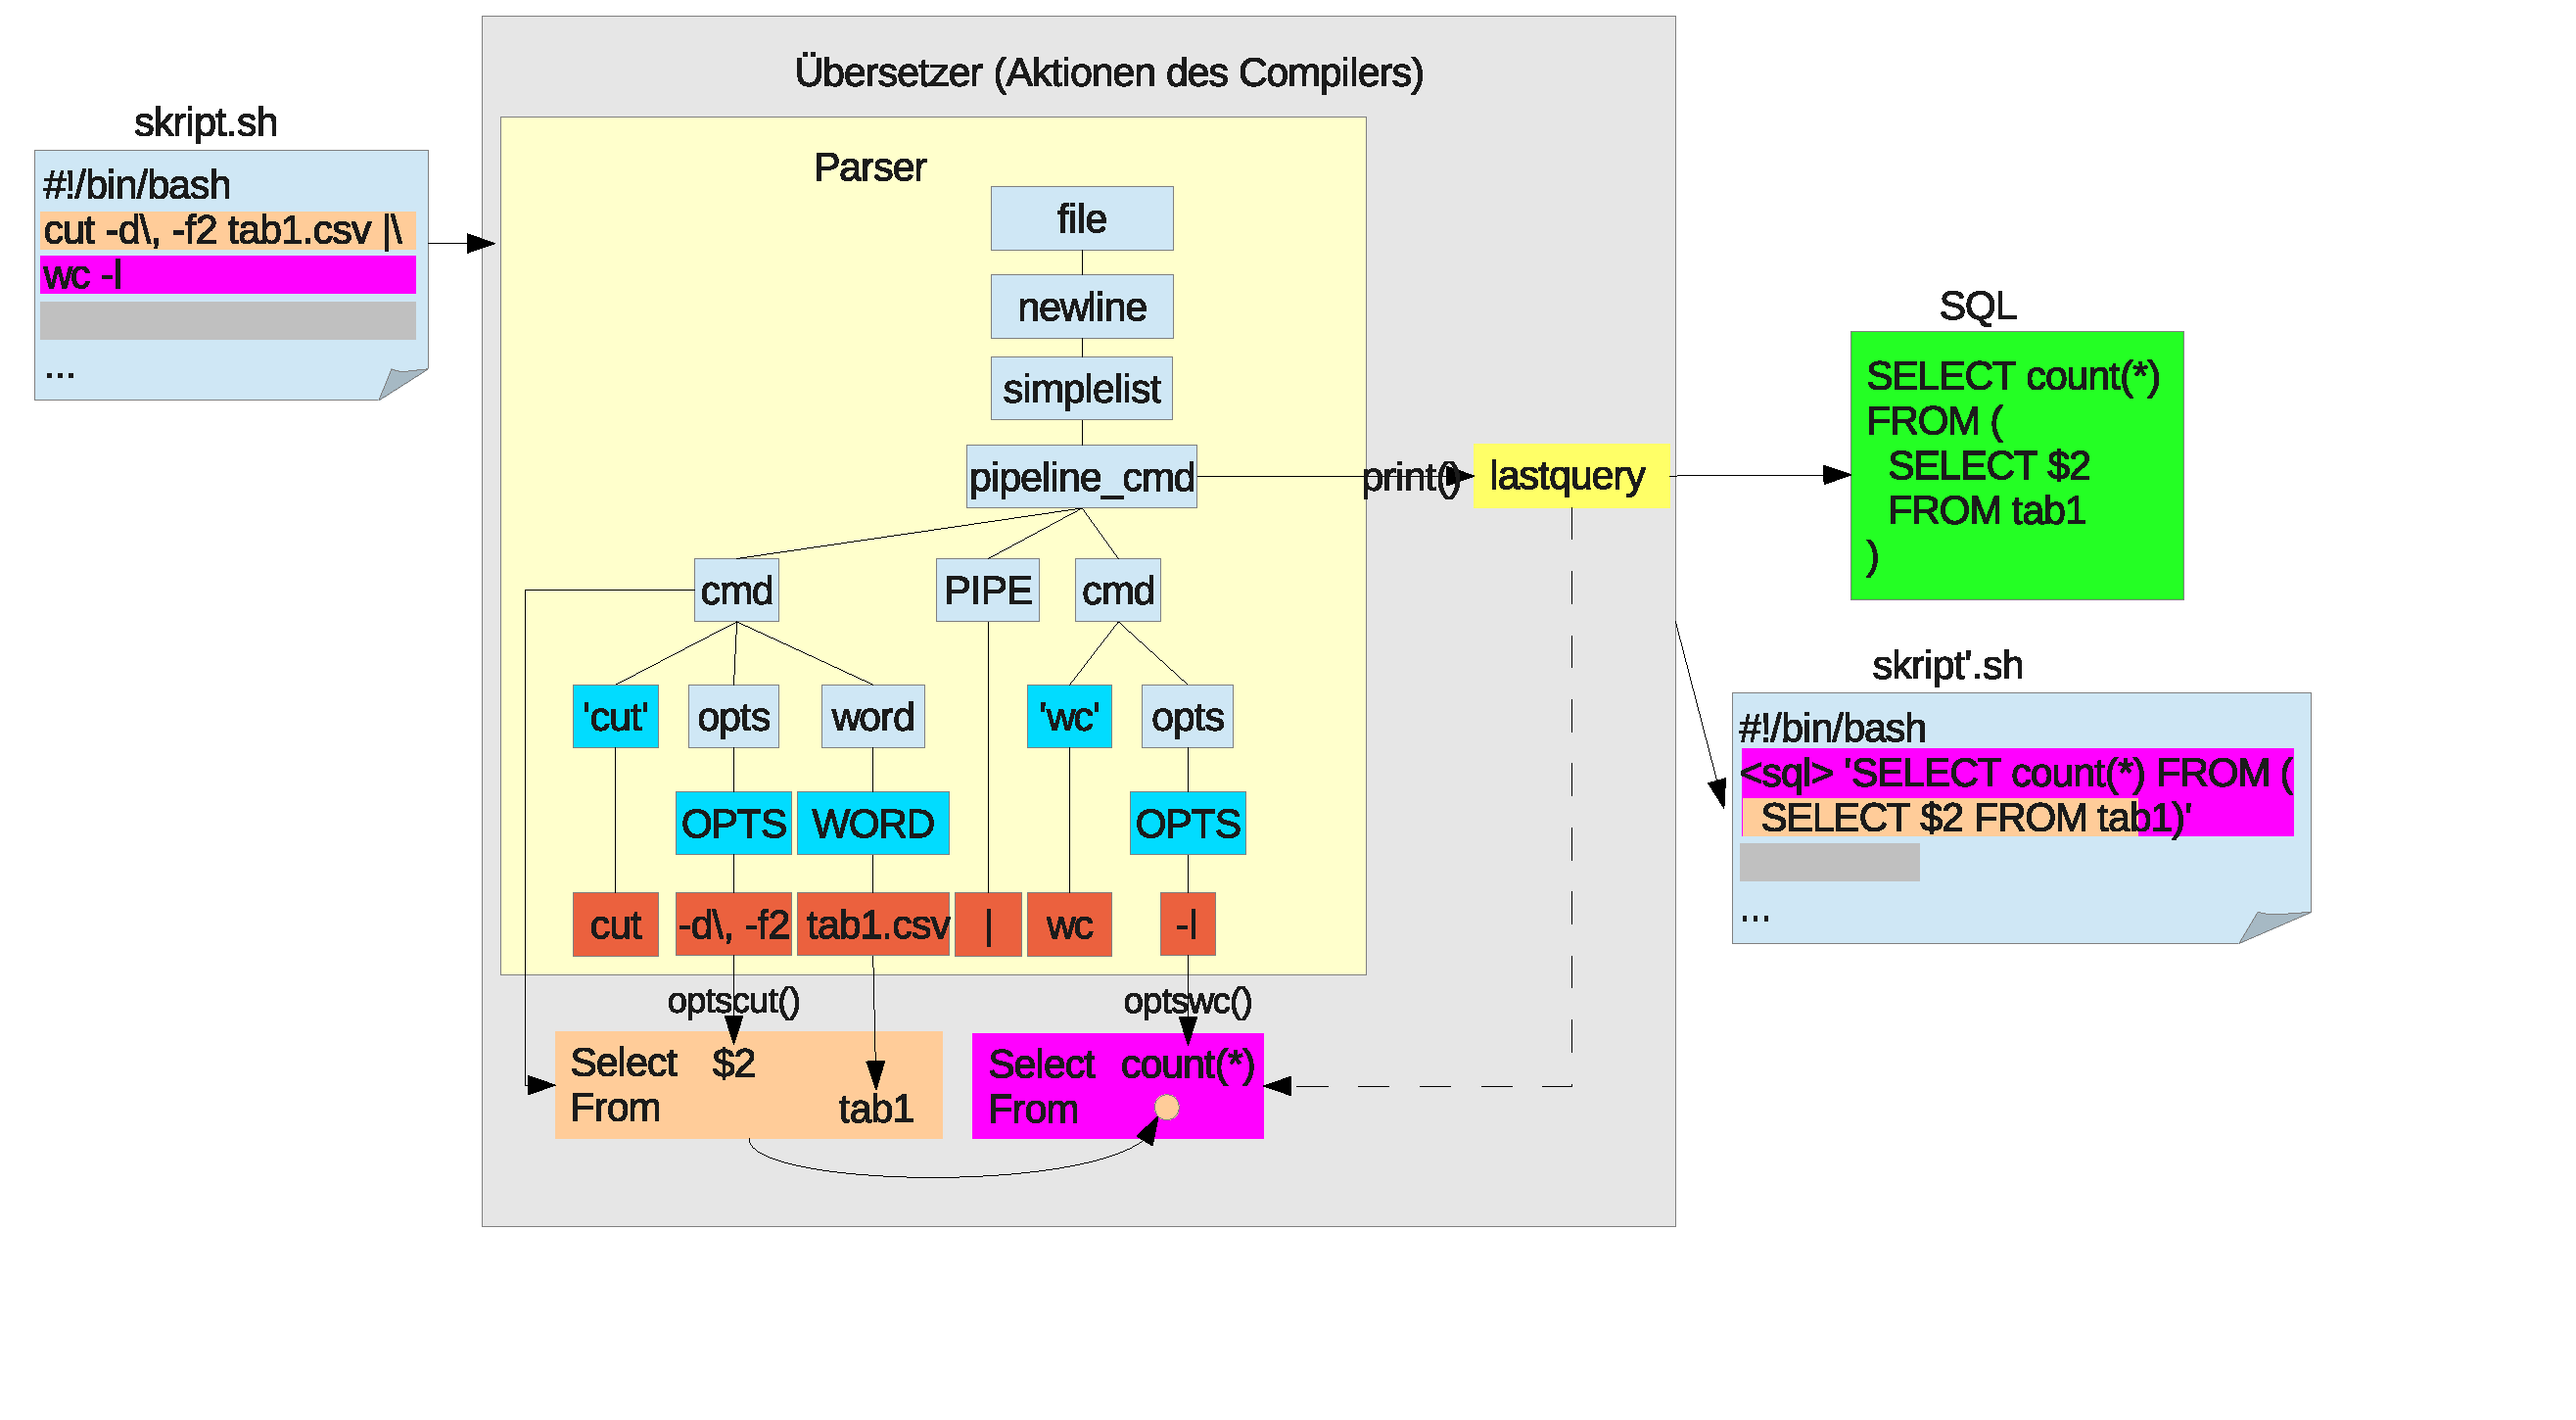
\includegraphics[scale=.4]{parsen.eps}
\caption{Parsen und Erstellen eine Syntaxbaums, anschließend Übersetzen}
\label{fig:parsen}
\end{figure}

Die Regel \textit{cmd} übernimmt zuerst die alte Abfrage, der Inhalt aus der Pipeline, also die zuletzt in SQL übersetzte Abfrage \textit{lastquery}, wird in einer temporären Variablen \textit{fromPipe} gespeichert. Eine Subshell kann Teil einer Abfrage sein, deshalb wird lastquery auf NULL gesetzt, damit geöffnetete Subshells mit leerer Eingabe beginnen, also ohne einen Input. Anschließend kann eine neue SQL-Abfrage erzeugt werden, in die das zu parsende Kommando übersetzt wird. Alle weiteren Attribute dienen zur Bearbeitung bei bestimmten Kommandos (z.B. Zählen der Argumente bei join). Immer wird ein stringstream benötigt, in den der Inhalt der Symbole geschrieben wird. Am Ende der Regel wird die gerade erzeugte Abfrage als aktuelle gesetzt, also in die globale Variable \textit{lastquery}.

\begin{lstlisting}[language=C++]
/* Rules for parsing bash command to SQL */
cmd returns [TheQuery *r]
@init{
        /* new TheQuery r,
        afterwards, set old query (lastquery) as table-reference
        set lastquery as null, so queries from subshell won't be
        included twice */
        TheQuery* fromPipe=lastquery;
        lastquery=NULL;
        r = new TheQuery();
        stringstream s;
        char buffer[80];
        int helpsize=0, join_on;
}
@after{
        /* query r is the most recent query  */
        lastquery=r;
}
\end{lstlisting}

\subsubsection{Das Kommando cut}
Da das Übersetzen der meisten Kommandos ähnlich erfolgt, wird \textit{cut} vorgestellt (s. Abb. \ref{fig:cut}).

\begin{figure}[h]
\centering
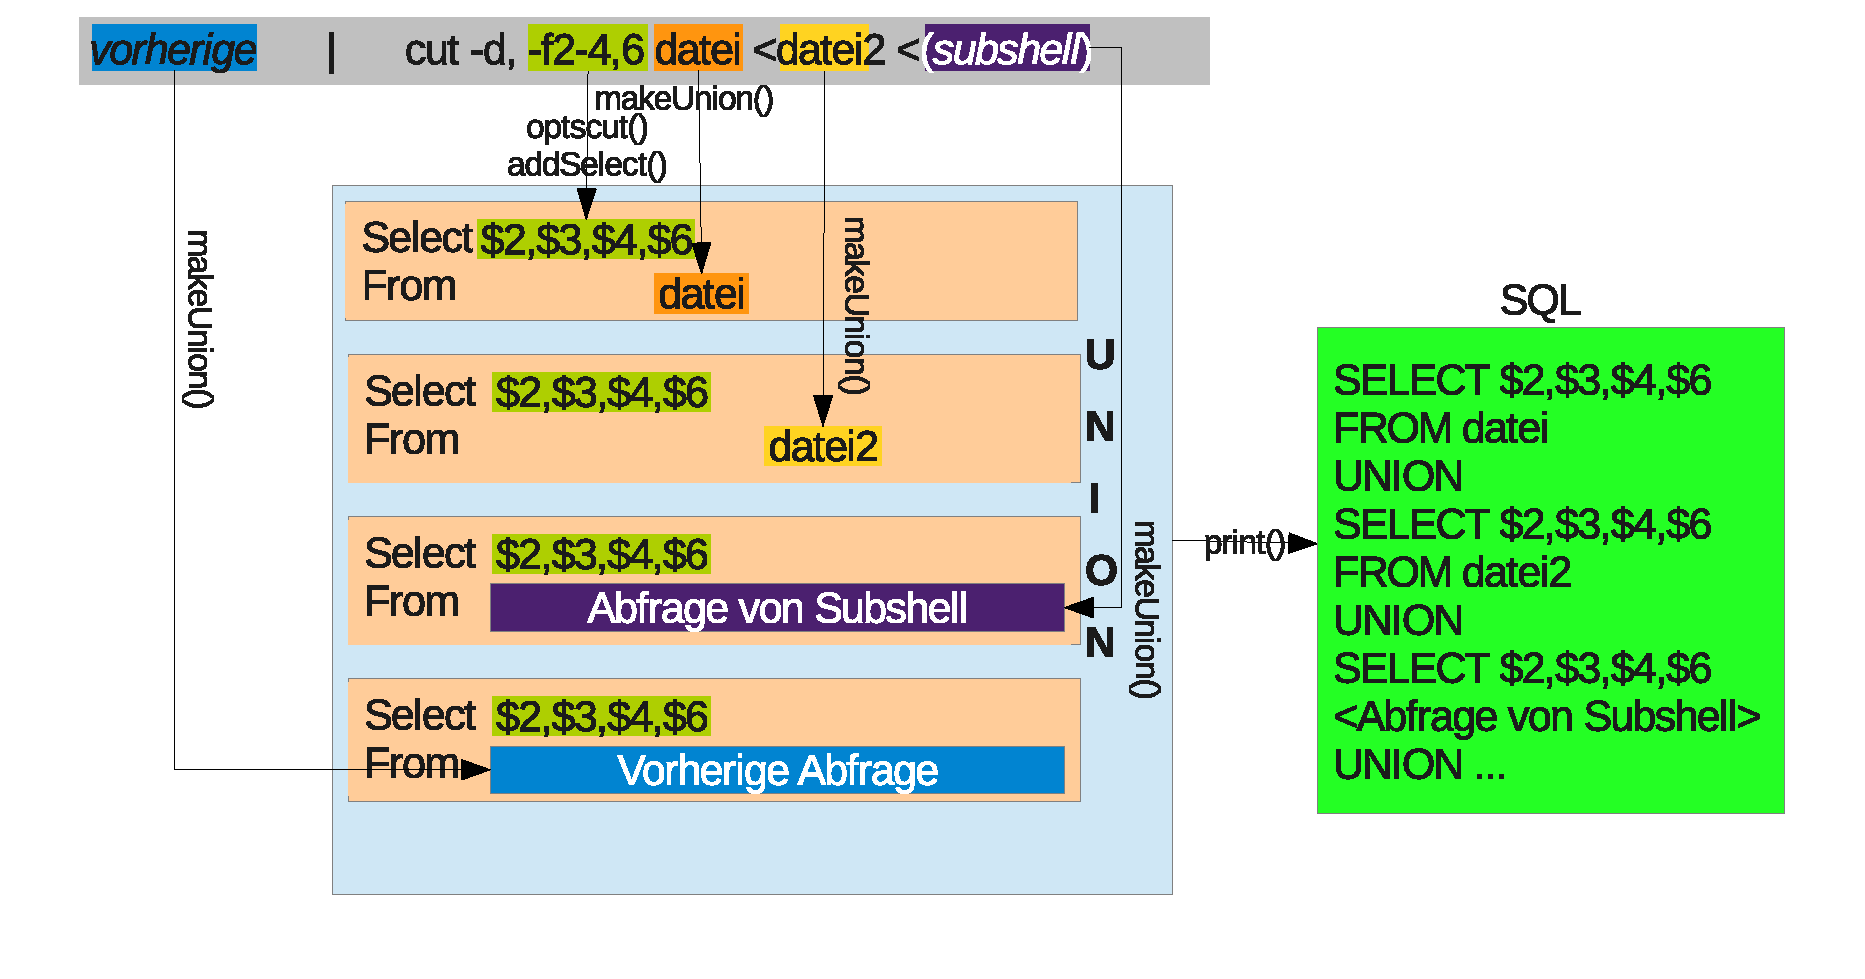
\includegraphics[scale=.4]{befehlcut.eps}
\caption{Konvertieren des Befehls cut in SQL}
\label{fig:cut}
\end{figure}

Zuerst wird immer das Kommando abgefragt, anschließend werden die Parameter geparst, also Optionen, die Eingabe oder die Umlenkung als Eingabe. Für jedes Kommando muss eine eigene Regel erstellt werden. Die Aktionen zu den Regeln sind recht schlicht, die Optionen, über das Symbol \textit{opts}, das für alle Zeichenfolgen steht, die mit '-' eingeleitet werden, werden mit der zugehörigen Funktion \lstinline{optscut()} geparst und in die Abfrage übersetzt.
Als Parameter kann eine Quelldatei stehen, die als Tabellenname angenommen wird. Dies passiert mit der Methode der Klasse TheQuery \lstinline{makeUnion()}, die im Falle mehrerer Tabellen die Vereinigung darüber bildet.
Am Ende wird die über die Pipeline erhaltene Abfrage berücksichtigt, auch sie wird mit \lstinline{makeUnion()} zur aktuellen Abfrage vereinigt.

\begin{lstlisting}[language=C++]
        :
          'cut'         ( opts
                                {
                                s.str(""); s.clear();
                                s << $opts.text; s.getline(buffer,80);
                                optscut(buffer,r);
                                }
                        | word
                                {
                                s.str(""); s.clear(); s << $word.text;
                                r->makeUnion(s.str());
                                }
                        | from_redir
                                {/* fname!=NULL, wenn Dateiname */
                                if (!$from_redir.fname.empty())
                                        r->makeUnion($from_redir.fname);
			          }
                        | '- '
                        )+
                        {r->makeUnion(fromPipe);}
\end{lstlisting}

Das Vereinigen von Tabellen mittels \lstinline{makeUnion()} ist für fast alle Befehle identisch, auch das Parsen der Optionen ist meist sehr ähnlich, darum werden noch drei besondere Befehle hervorgehoben.

\subsubsection{Das Kommando grep}

\begin{figure}[h]
\centering
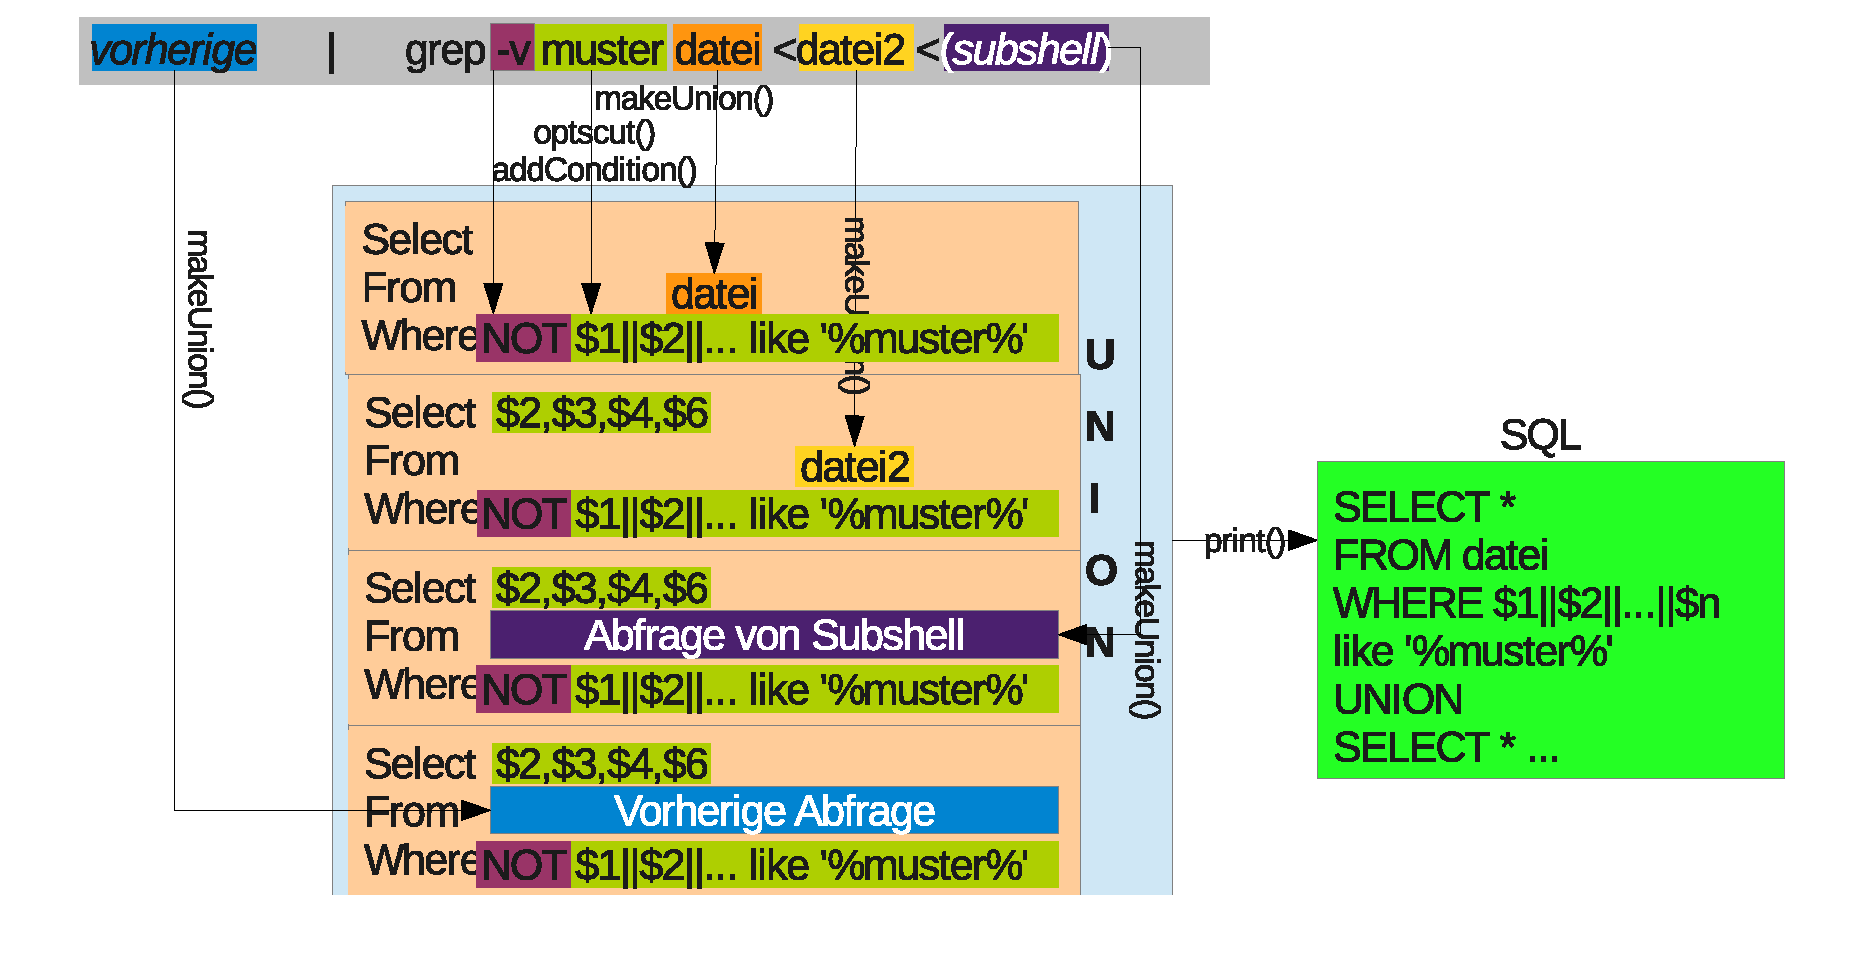
\includegraphics[scale=.4]{befehlgrep.eps}
\caption{Konvertieren des Befehls grep in SQL}
\label{fig:grep}
\end{figure}

Für den Befehl grep ist das angegebene Suchmuster mit allen Feldern zu vergleichen, daher werden zuerst alle Felder konkateniert (hier ist also die gesamte Anzahl an Spalten nötig) und danach wird mit \textit{like} nach Vorkommen des Musters darin gesucht. Da in grep eventuell auch das Spaltentrennzeichen mit angegeben ist, kann beim Verbinden der Felder auch das Trennzeichen berücksichtigt werden (\lstinline{$1||,||$2}).
Der erzeugte Ausdruck ist dabei in alle aktuellen Abfragen einzubinden.

\subsubsection{Das Kommando join}

\begin{figure}[h]
\centering
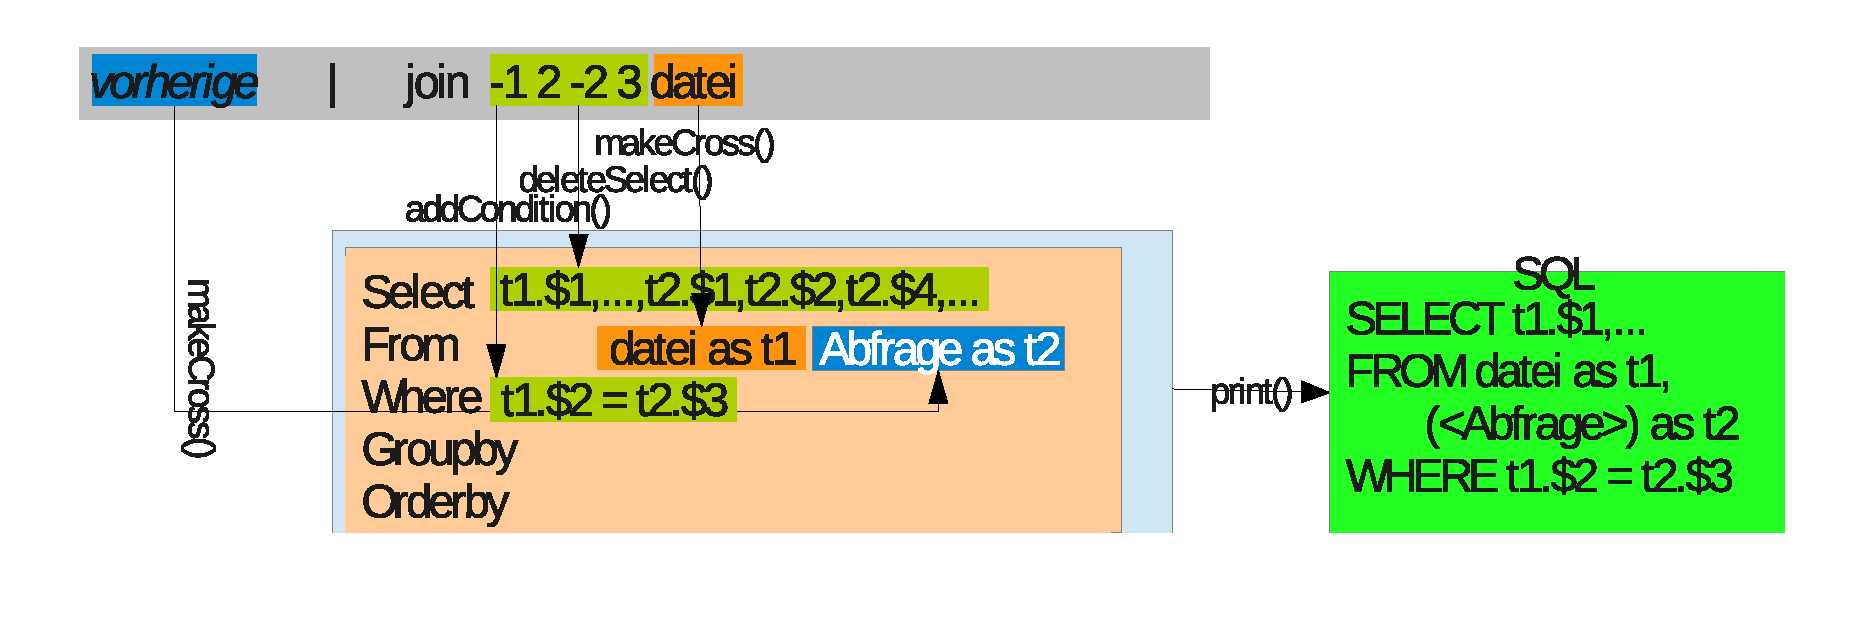
\includegraphics[scale=.4]{befehljoin.eps}
\caption{Konvertieren des Befehls join in SQL}
\label{fig:join}
\end{figure}

Der Verbund kann so in SQL übernommen werden, die zu verbindenden Spalten werden mit den Optionen \textit{-1} und \textit{-2} angegeben (ohne Angabe von Optionen wird über die jeweils erste Spalte verbunden), zu berücksichtigen ist noch die Reihenfolge der Tabellen, ob an erster oder zweiter Stelle, und dass die verbundene Spalte der zweiten Tabelle nicht im Ergebnis auftaucht. Um das Verbinden zu erleichtern, werden die beiden Tabellen noch mit einem Bezeichner versehen (t1, t2). Da keine Vereinigung sondern ein Join gebildet werden soll, erfolgt das Hinzufügen der Tabellen in die From-Klausel mittels \lstinline{makeCross()}.

\subsubsection{Ausdrücke der Sprache awk}

\begin{figure}[h]
\centering
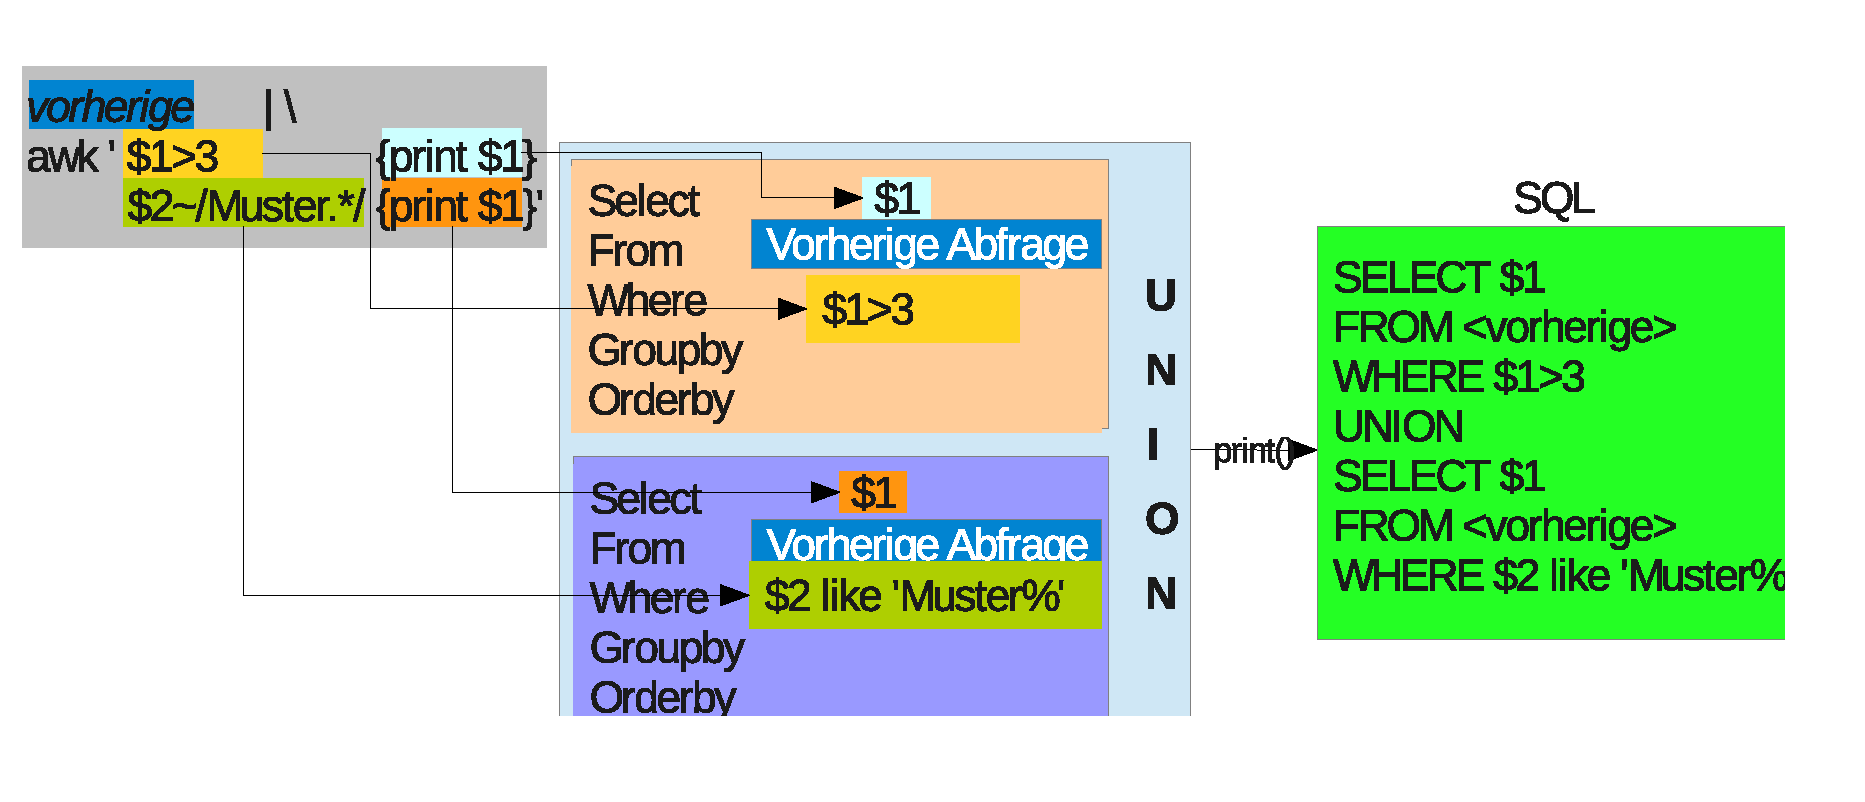
\includegraphics[scale=.4]{befehlawk.eps}
\caption{Konvertieren des Befehls awk in SQL}
\label{fig:awk}
\end{figure}

Das Programm übersetzt auch einfache Konstrukte der Sprache awk. Da sie meist aus einem Muster und einer folgenden Anweisung bestehen, kann das Muster als Bedingung und die Anweisung in die Select-Klausel übernommen werden. Besteht ein Suchmuster aus einem einfachen Vergleich wie
\lstinline{$2 == "Inhalt"},
so kann das Muster direkt in die Bedingung übernommen werden, lediglich die Kennzeichnung von Zeichenketten durch einfache Hochkommata und die Äquivalenz durch ein einfaches '=' müssen angepasst werden (\lstinline{$2 = 'Inhalt'}). Reguläre Ausdrucke sind ähnlich anzupassen (\lstinline{$2 ~/.Muster.*/}), da sie, identisch zu grep, dem \textit{like}-Operator entsprechen (\lstinline{$2 like '?Muster\%'}).
Da nach jedem Muster eine andere Aktion folgt, sind diese auch als unabhängige Anfragen zu betrachten, für jedes Muster muss eine erneute Abfrage desselben Ursprungs mit identischen From-Klauseln erstellt werden. In die Select-Klausel wird jedes \lstinline{print} übersetzt, denn nur da erfolgt eine Ausgabe. Im Moment werden nur Ausgaben der Felder unterstützt wie \lstinline{print $1, $2}, kompliziertere arithmetische Ausdrücke und Ausgabe von Variablen müssten in eine entsprechende Anweisung mit \textit{case} umgewandelt werden.

\subsection{Bedienung}
Im Ordner \textit{plus\_bash\_parser\_antlr} liegen die Grammatikdatei \textit{SimpleBashSQL.g}, die Dateien TheQuery.hpp und -.cpp, eine dynamische Bibliothek und ein Makefile. Wie im vorherigen Fall wird der Compiler automatisch generiert, wenn die Konfiguration richtig erfolgt ist. Alternativ kann das init-Skript angepasst werden, das die Pfade richtig setzt.
\begin{lstlisting}[language=Bash]
$ . ./init
\end{lstlisting}

ANTLR erzeugt eine Lexer- und eine Parser-Quelldatei \textit{SimpleBashSQL\{Lexer,Parser\}.}

\textit{\{hpp,cpp\}}, die zu dem fertigen Compiler mittels \textit{g++} kompiliert werden.

\begin{lstlisting}[language=make]
simplebashsql: theparser thequery.o
        g++ -std=c++11 -g -o $@ $(CFLAGS) -lantlr3c $(OBJ)Parser.cpp $(OBJ)Lexer.cpp thequery.o
        rm thequery.o
\end{lstlisting}

Das Programm nimmt den Dateinamen eines Skripts als Eingabeparameter und schickt das Ergebnis auf die Standardausgabe. So wird das Skript:
\begin{lstlisting}[language=Bash]
$ cat testskript.sh
#!/bin/bash
cut -f1,2,3 vorlesungen.csv | sort -k2
\end{lstlisting}
übersetzt in:
\begin{lstlisting}[language=Bash]
$ ./simplebashsql testskript.sh
SELECT * FROM (SELECT $1,$2,$3 FROM vorlesungen.csv as t1 ) as t1  ORDER BY $2
\end{lstlisting}

Existiert darüber hinaus eine Datei vorlesungen.csv mit Kopfzeile, so erkennt das Programm gleich die Spaltenbezeichner und erzeugt sprechende Namen.
\begin{lstlisting}[language=Bash]
$ head -1 vorlesungen.csv
VorlNr,Titel,SWS,
$ ./simplebashsql testskript.sh
SELECT * FROM (SELECT VorlNr,Titel,SWS FROM vorlesungen.csv as t1 ) as t1  ORDER BY Titel
\end{lstlisting}

\subsection{Rückübersetzung einer TPC-H Abfrage}
Um wieder zu den TPC-H Abfragen zurückzukehren, so genügen die definierten Regeln um die anfangs beschriebene vierte Abfrage wieder zurückzuübersetzen.
\begin{lstlisting}[language=Bash]
$ ./simplebashsql query4b
mkfifo tmporder.csv
WITH tmporder.csv AS (
SELECT $1,$6 FROM (SELECT * FROM orders.csv as t1  UNION SELECT * FROM (SELECT * FROM orders.tbl as t1  ORDER BY $1,$1) as t1union1 ) as t1  WHERE (true) AND ($5<'1993-10-01') AND ($5>='1993-07-01')  )

WITH tmpline.csv AS (
SELECT $1 FROM (SELECT $1 FROM (SELECT * FROM lineitem.csv as t1  UNION SELECT * FROM (SELECT * FROM lineitem.tbl as t1  ORDER BY $1,$1) as t1union1 ) as t1  WHERE (true) AND ($12<$13) ) as t1  GROUP BY $1 )

SELECT count(*),$2 FROM (SELECT * FROM (SELECT * FROM (SELECT $2 FROM (SELECT $1,$2,$3,$4,$5,$6,$7,$8,$9 FROM tmporder.csv as t1, tmpline.csv as t2  WHERE (t1.$1=t2.$10) ) as t1 ) as t1 ) as t1 ) as t1  GROUP BY $2
rm tmp*.csv
\end{lstlisting}

Im Moment erscheinen noch kryptische Spaltenbezeichner, denn die Dateien konnten noch nicht gefunden werden, der Übersetzer nimmt für jede Tabelle die definierten neun Spalten an. Für jede eingelesene Datei muss jetzt eine Datei mit Kopfzeilen definiert sein, für Abfragen innerhalb einer Vereinigung genügt die Existenz einer Datei (orders.csv gibt für orders.tbl mit die Spalten an). Leider erzeugt das Programm noch keine solche Datei für Hilfstabellen, die das Skript erzeugt. Folglich müssen für tmporder.csv und tmpline.csv auch Dateien hinterlegt werden (das ursprüngliche Skript ist ausgeführt worden um an die Dateien zu gelangen).
\begin{lstlisting}[language=Bash]
$ cat orders.csv 
o_orderkey,o_custkey,o_orderstatus,o_totalprice,o_orderdate,o_orderpriority,o_clerk,o_shippriority,o_comment,
$ cat orders.csv 
o_orderkey,o_custkey,o_orderstatus,o_totalprice,o_orderdate,o_orderpriority,o_clerk,o_shippriority,o_comment,
$ cat lineitem.csv 
l_orderkey,l_partkey,l_suppkey,l_linenumber,l_quantity,l_extendedprice,l_discount,l_tax,l_returnflag,l_linestatus,l_shipdate,l_commitdate,l_receiptdate,l_shipinstruct,l_shipmode,l_comment,
$ cat tmporder.csv 
o_orderkey,o_orderpriority,
$ cat tmpline.csv 
l_orderkey,
$ ./simplebashsql query4b
\end{lstlisting}\begin{lstlisting}[language=SQL]
mkfifo tmporder.csv
WITH tmporder.csv AS (
SELECT o_orderkey,o_orderpriority FROM (SELECT * FROM orders.csv as t1  UNION SELECT * FROM (SELECT * FROM orders.tbl as t1  ORDER BY $1,$1) as t1union1 ) as t1  WHERE (true) AND (o_orderdate<'1993-10-01') AND (o_orderdate>='1993-07-01')  )

WITH tmpline.csv AS (
SELECT l_orderkey FROM (SELECT l_orderkey FROM (SELECT * FROM lineitem.csv as t1  UNION SELECT * FROM (SELECT * FROM lineitem.tbl as t1  ORDER BY $1,$1) as t1union1 ) as t1  WHERE (true) AND (l_commitdate<l_receiptdate) ) as t1  GROUP BY l_orderkey )

SELECT count(*),o_orderpriority FROM (SELECT * FROM (SELECT * FROM (SELECT o_orderpriority FROM (SELECT o_orderkey,o_orderpriority FROM tmporder.csv as t1, tmpline.csv as t2  WHERE (t1.o_orderkey=t2.l_orderkey) ) as t1 ) as t1 ) as t1 ) as t1  GROUP BY o_orderpriority
rm tmp*.csv
\end{lstlisting}

Diese Abfrage kann nun über eine SQL-Schnittstelle eingegeben werden, vorher müssen die Dateiendungen entfernt werden (.csv), die manche SQL-Inline-Tools jedoch benötigen, anschließend kann die Zeit gemessen werden (Zeiten der ersten und letzten Abfrage sind der HyPer-Webschnittstelle entnommen).

\begin{center}
\begin{tabular}{|l|r|}
Abfrage & Zeit \\ \hline
Query4 original & 62.87\ ms\\
Query4b Skript &  21\ 910,00\ ms\\
Query4b bash2sql & 5\ 946.87\ ms
\end{tabular}
\end{center}

		
		%\part[Ausblick]{Ausblick}
		\chapter{Ausblick}
Diese Arbeit hat gezeigt, dass die Datenanalyse in der Wissenschaft durch den Einsatz relationaler Datenbanksysteme verbessert werden kann. Bestehende Bash-Skripte, die bislang bei der Analyse den Vorzug erhalten haben, können automatisiert in SQL übersetzt werden, den Grundstein hierfür hat diese Arbeit gelegt.
Der vorgestellte Übersetzer parst die Bash-Syntax bis auf Funktionen und kann grundlegende Kommandos in SQL übersetzen. Bei der Weiterentwicklung des Übersetzers sollte in Erwägung gezogen werden einen AST (abstrakter Syntaxbaum) explizit zu generieren, sodass die Übersetzungslogik vom Parsen unabhängig ist.
Außerdem hat die Arbeit durch die Implementierung des TPC-H Skriptes verfügbare Skripte geliefert, die bei Weiterentwicklungen eines Übersetzers als Testdaten dienen können.
\section{Schleifen}
Bisher wurde nicht mit Schleifen experimentiert. Da eine Schleife immer als Ganzes eingelesen wird, führt dies zu Problemen, da zuerst die Kommandos im Rumpf bearbeitet werden, am Ende die Schleife selber. Bisher regelte dies eine globale Variable, die speichert, in welcher Ebene sich das Kommando befindet. Dies sollte bei zukünftigen Entwicklungen verbessert werden.

\section{Sprache awk separat}
Im Moment erfolgt das Parsen von awk-Ausdrücken innerhalb der Bash-Grammatik, obwohl diese grundverschieden sind, so spielen in awk Leerräume keine Rolle, in Bash schon. Daher sollte überlegt werden, Teile an einen externen Parser zu übergeben, der dann auch eine Abfrage als Objekt der Klasse TheQuery zurückgibt.

\section{Vor Übersetzen zusammenfügen}
Im Moment werden zuerst die Kommandos und in Abhängigkeit dieses alle weiteren Parameter (Optionen, Eingaben, Subshells) eingelesen, bei Umstieg auf einen AST sollten die Kommandos zuerst geparst und dann wieder zusammengesetzt werden. Die Optionen sollten mit \textit{getopts()} abgefragt werden, die Logik zum Erkennen der Befehle stünde dann in einer Methode durch Auswahl nach dem Befehlsnamen. (s. Abb. \ref{fig:improve})

\begin{figure}
\centering
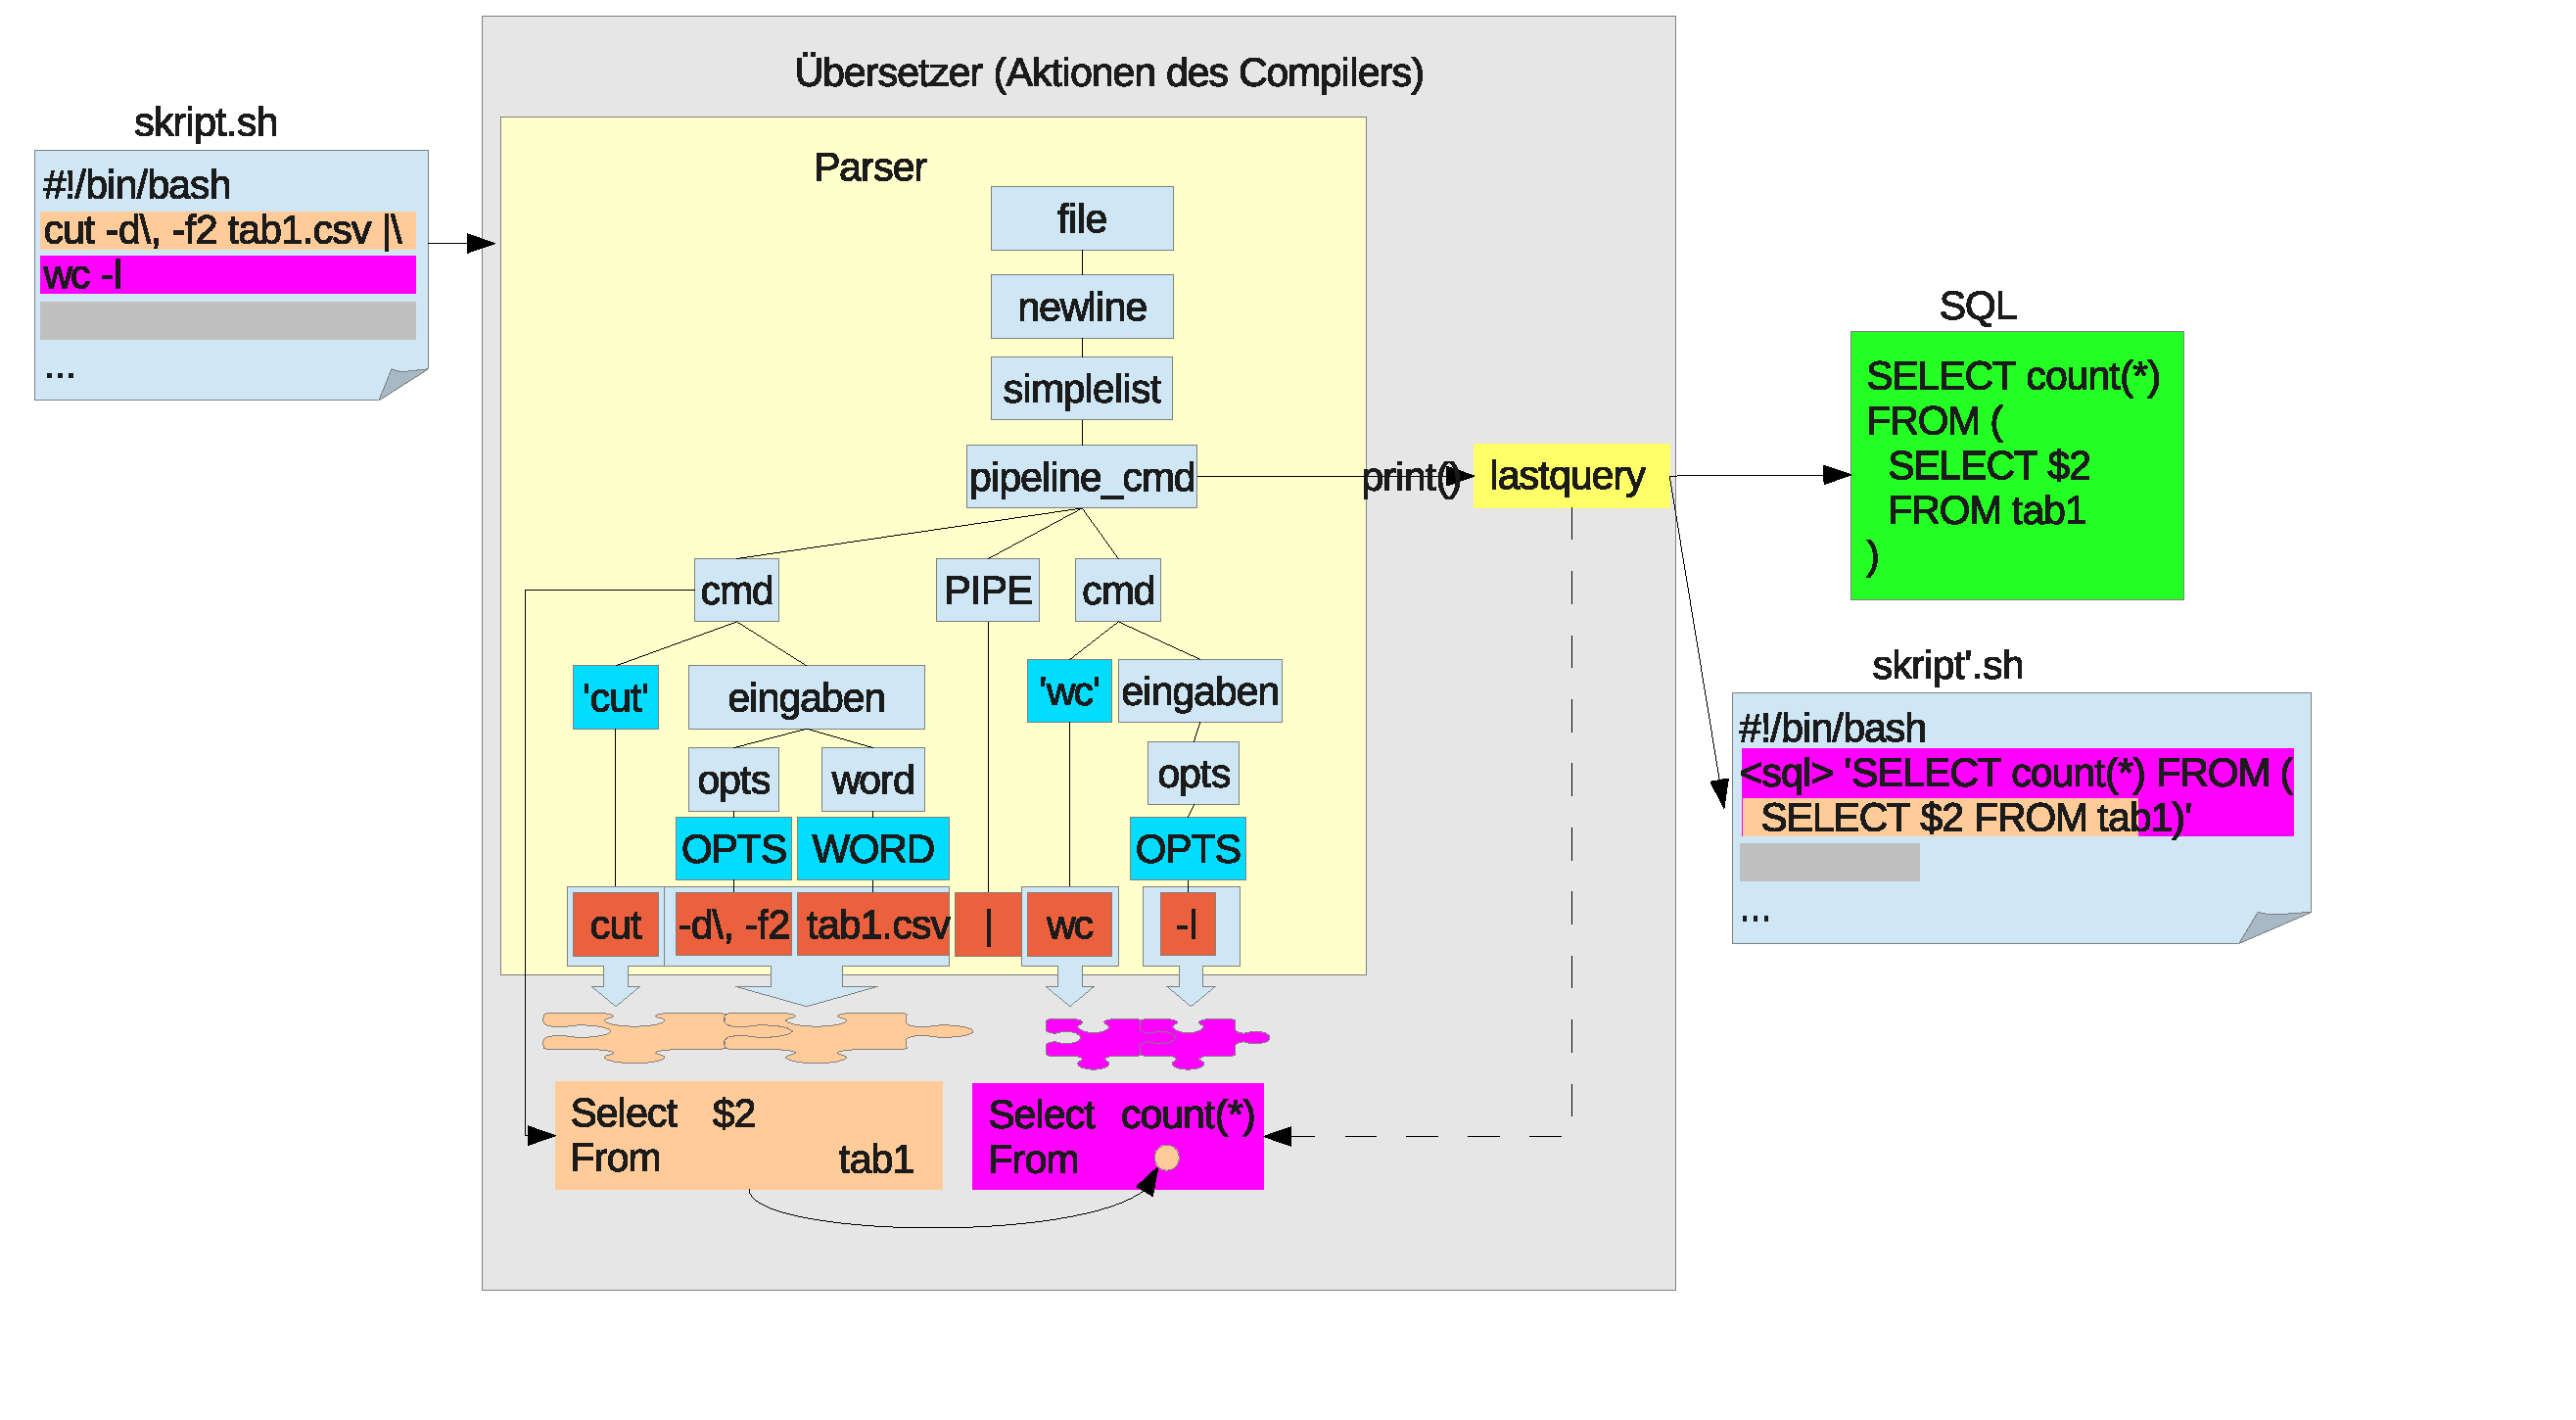
\includegraphics[scale=.4]{parsen_improve.eps}
\caption{Vorheriges Zusammenführen der Befehle}
\label{fig:improve}
\end{figure}

\section{Fazit}
Insgesamt ist es gelungen einen Vergleich aufzustellen, der die Laufzeit von Bash-Skripten analysiert. Es gibt einen Weg, die Abfragen zu übersetzen, und noch genug Platz für Ideen, um alle möglichen Skripte übersetzen zu können.
Diese Arbeit hat gezeigt, dass sich der Umstieg auf SQL lohnt, und will ermutigen, diesen Weg weiter zu verfolgen.

		% ---------------------------------------------------------------------------
		%
		% Appendix
		%
		% ---------------------------------------------------------------------------
		
		\part*{Appendix}
		\addcontentsline{toc}{part}{Appendix}
		
		\appendix %---------------------------------------
		
	\chapter{TPC-H-Abfragen}
\section{Abfragen}
\subsection*{Abfrage 1}
\lstinputlisting[language=Bash]{../01Anfang/im-giga/query1}
%\newpage
\subsection*{Abfrage 2}
\lstinputlisting[language=Bash]{../01Anfang/im-giga/query2}
\newpage
\subsection*{Abfrage 3}
\lstinputlisting[language=Bash]{../01Anfang/im-giga/query3}
%\newpage
\subsection*{Abfrage 4}
\lstinputlisting[language=Bash]{../01Anfang/im-giga/query4}
%\newpage
\subsection*{Abfrage 5}
\lstinputlisting[language=Bash]{../01Anfang/im-giga/query5}
%\newpage
\subsection*{Abfrage 6}
\lstinputlisting[language=Bash]{../01Anfang/im-giga/query6}
%\newpage
\subsection*{Abfrage 7}
\lstinputlisting[language=Bash]{../01Anfang/im-giga/query7}
%\newpage
\subsection*{Abfrage 8}
\lstinputlisting[language=Bash]{../01Anfang/im-giga/query8}
%\newpage
\subsection*{Abfrage 9}
\lstinputlisting[language=Bash]{../01Anfang/im-giga/query9}
%\newpage
\subsection*{Abfrage 10}
\lstinputlisting[language=Bash]{../01Anfang/im-giga/query10}
%\newpage
\subsection*{Abfrage 11}
\lstinputlisting[language=Bash]{../01Anfang/im-giga/query11}
%\newpage
\subsection*{Abfrage 12}
\lstinputlisting[language=Bash]{../01Anfang/im-giga/query12}
%\newpage
\subsection*{Abfrage 13}
\lstinputlisting[language=Bash]{../01Anfang/im-giga/query13}
%\newpage
\subsection*{Abfrage 14}
\lstinputlisting[language=Bash]{../01Anfang/im-giga/query14}
%\newpage
\subsection*{Abfrage 15}
\lstinputlisting[language=Bash]{../01Anfang/im-giga/query15}
%\newpage
\subsection*{Abfrage 16}
\lstinputlisting[language=Bash]{../01Anfang/im-giga/query16}
%\newpage
\subsection*{Abfrage 17}
\lstinputlisting[language=Bash]{../01Anfang/im-giga/query17}
%\newpage
\subsection*{Abfrage 18}
\lstinputlisting[language=Bash]{../01Anfang/im-giga/query18}
%\newpage
\subsection*{Abfrage 19}
\lstinputlisting[language=Bash]{../01Anfang/im-giga/query19}
%\newpage
\subsection*{Abfrage 20}
\lstinputlisting[language=Bash]{../01Anfang/im-giga/query20}
%\newpage
\subsection*{Abfrage 21}
\lstinputlisting[language=Bash]{../01Anfang/im-giga/query21}
%\newpage
\subsection*{Abfrage 22}
\lstinputlisting[language=Bash]{../01Anfang/im-giga/query22}
%\newpage

\section{Parallelisierte Abfragen}
\subsection*{Abfrage 2}
\lstinputlisting[language=Bash]{../01Anfang/im-giga/query2p}
%\newpage
\subsection*{Abfrage 3}
\lstinputlisting[language=Bash]{../01Anfang/im-giga/query3p}
%\newpage
\subsection*{Abfrage 4a}
\lstinputlisting[language=Bash]{../01Anfang/im-giga/query4a}
%\newpage
\subsection*{Abfrage 4b}
\lstinputlisting[language=Bash]{../01Anfang/im-giga/query4b}
%\newpage
\subsection*{Abfrage 5}
\lstinputlisting[language=Bash]{../01Anfang/im-giga/query5p}
%\newpage
\subsection*{Abfrage 7}
\lstinputlisting[language=Bash]{../01Anfang/im-giga/query7p}
\newpage
\subsection*{Abfrage 8}
\lstinputlisting[language=Bash]{../01Anfang/im-giga/query8p}
%\newpage
\subsection*{Abfrage 9}
\lstinputlisting[language=Bash]{../01Anfang/im-giga/query9p}
%\newpage
\subsection*{Abfrage 10}
\lstinputlisting[language=Bash]{../01Anfang/im-giga/query10p}
%\newpage
\subsection*{Abfrage 11}
\lstinputlisting[language=Bash]{../01Anfang/im-giga/query11p}
%\newpage
\subsection*{Abfrage 12}
\lstinputlisting[language=Bash]{../01Anfang/im-giga/query12p}
%\newpage
\subsection*{Abfrage 13}
\lstinputlisting[language=Bash]{../01Anfang/im-giga/query13p}
%\newpage
\subsection*{Abfrage 14}
\lstinputlisting[language=Bash]{../01Anfang/im-giga/query14p}
%\newpage
\subsection*{Abfrage 15}
\lstinputlisting[language=Bash]{../01Anfang/im-giga/query15p}
%\newpage
\subsection*{Abfrage 16}
\lstinputlisting[language=Bash]{../01Anfang/im-giga/query16p}
%\newpage
\subsection*{Abfrage 17}
\lstinputlisting[language=Bash]{../01Anfang/im-giga/query17p}
%\newpage
\subsection*{Abfrage 18}
\lstinputlisting[language=Bash]{../01Anfang/im-giga/query18p}
%\newpage
\subsection*{Abfrage 19}
\lstinputlisting[language=Bash]{../01Anfang/im-giga/query19p}
%\newpage
\subsection*{Abfrage 20}
\lstinputlisting[language=Bash]{../01Anfang/im-giga/query20p}
%\newpage
\subsection*{Abfrage 21}
\lstinputlisting[language=Bash]{../01Anfang/im-giga/query21p}
%\newpage
\subsection*{Abfrage 22}
\lstinputlisting[language=Bash]{../01Anfang/im-giga/query22p}
%\newpage

\chapter{datamash Abfragen}
\subsection*{Abfrage 1}
\lstinputlisting[language=Bash]{../01Anfang/datamash-giga/query1}
%\newpage
\subsection*{Abfrage 2}
\lstinputlisting[language=Bash]{../01Anfang/datamash-giga/query2}
%\newpage
\subsection*{Abfrage 3}
\lstinputlisting[language=Bash]{../01Anfang/datamash-giga/query3}
%\newpage
\subsection*{Abfrage 4}
\lstinputlisting[language=Bash]{../01Anfang/datamash-giga/query4}
%\newpage
\subsection*{Abfrage 5}
\lstinputlisting[language=Bash]{../01Anfang/datamash-giga/query5}
%\newpage
\subsection*{Abfrage 6}
\lstinputlisting[language=Bash]{../01Anfang/datamash-giga/query6}
%\newpage
\subsection*{Abfrage 7}
\lstinputlisting[language=Bash]{../01Anfang/datamash-giga/query7}
%\newpage
\subsection*{Abfrage 8}
\lstinputlisting[language=Bash]{../01Anfang/datamash-giga/query8}
%\newpage
\subsection*{Abfrage 9}
\lstinputlisting[language=Bash]{../01Anfang/datamash-giga/query9}
%\newpage
\subsection*{Abfrage 10}
\lstinputlisting[language=Bash]{../01Anfang/datamash-giga/query10}
%\newpage
\subsection*{Abfrage 11}
\lstinputlisting[language=Bash]{../01Anfang/datamash-giga/query11}
%\newpage
\subsection*{Abfrage 12}
\lstinputlisting[language=Bash]{../01Anfang/datamash-giga/query12}
%\newpage
\subsection*{Abfrage 13}
\lstinputlisting[language=Bash]{../01Anfang/datamash-giga/query13}
%\newpage
\subsection*{Abfrage 14}
\lstinputlisting[language=Bash]{../01Anfang/datamash-giga/query14}
%\newpage
\subsection*{Abfrage 15}
\lstinputlisting[language=Bash]{../01Anfang/datamash-giga/query15}
%\newpage
\subsection*{Abfrage 16}
\lstinputlisting[language=Bash]{../01Anfang/datamash-giga/query16}
%\newpage
\subsection*{Abfrage 17}
\lstinputlisting[language=Bash]{../01Anfang/datamash-giga/query17}
%\newpage
\subsection*{Abfrage 18}
\lstinputlisting[language=Bash]{../01Anfang/datamash-giga/query18}
%\newpage
\subsection*{Abfrage 19}
\lstinputlisting[language=Bash]{../01Anfang/datamash-giga/query19}
%\newpage
\subsection*{Abfrage 20}
\lstinputlisting[language=Bash]{../01Anfang/datamash-giga/query20}
%\newpage
\subsection*{Abfrage 21}
\lstinputlisting[language=Bash]{../01Anfang/datamash-giga/query21}
%\newpage
\subsection*{Abfrage 22}
\lstinputlisting[language=Bash]{../01Anfang/datamash-giga/query22}
%\newpage


%\chapter{Der Bash2SQL-Compiler}
%\section{Yacc und Lex}
%\subsection*{Makefile}
%\lstinputlisting[language=make]{../02Parser/bash_parser_yacc/Makefile}
%\subsection*{bash2sql.lex}
%\lstinputlisting[language=C]{../02Parser/bash_parser_yacc/bash2sql.lex}
%\subsection*{bash2sql.y}
%\lstinputlisting[language=C]{../02Parser/bash_parser_yacc/bash2sql.y}
%
%\section{ANTLR mit C}
%\subsection*{Makefile}
%\lstinputlisting[language=make]{../02Parser/c_bash_parser_antlr/Makefile}
%\subsection*{SimpleBashSQL.g}
%\lstinputlisting[language=C]{../02Parser/c_bash_parser_antlr/SimpleBashSQL.g}
%
%\section{ANTLR mit C++}
%\subsection*{Makefile}
%\lstinputlisting[language=make]{../02Parser/plus_bash_parser_antlr/Makefile}
%\subsection*{Query.hpp}
%\lstinputlisting[language=C++]{../02Parser/plus_bash_parser_antlr/thequery.hpp}
%\subsection*{Query.cpp}
%\lstinputlisting[language=C++]{../02Parser/plus_bash_parser_antlr/thequery.cpp}
%\subsection*{SimpleBashSQL.g}
%\lstinputlisting[language=C++]{../02Parser/plus_bash_parser_antlr/SimpleBashSQL.g}

		
	


  \clearemptydoublepage
  
	\bibliography{bibliography/literature}
	
 
\end{document}

